\documentclass[10pt]{article}

\usepackage{jls_base}
\title{Decentralized Infrastructure for Neuro(science)}
\author{Jonny L. Saunders}
\date{\today}
\addbibresource{../assets/infrastructure.bib}
% Options for packages loaded elsewhere

\usepackage{color}
\usepackage{fancyvrb}
\newcommand{\VerbBar}{|}
\newcommand{\VERB}{\Verb[commandchars=\\\{\}]}
\DefineVerbatimEnvironment{Highlighting}{Verbatim}{commandchars=\\\{\}}
% Add ',fontsize=\small' for more characters per line
\newenvironment{Shaded}{}{}
\newcommand{\AlertTok}[1]{\textcolor[rgb]{1.00,0.00,0.00}{\textbf{#1}}}
\newcommand{\AnnotationTok}[1]{\textcolor[rgb]{0.38,0.63,0.69}{\textbf{\textit{#1}}}}
\newcommand{\AttributeTok}[1]{\textcolor[rgb]{0.49,0.56,0.16}{#1}}
\newcommand{\BaseNTok}[1]{\textcolor[rgb]{0.25,0.63,0.44}{#1}}
\newcommand{\BuiltInTok}[1]{#1}
\newcommand{\CharTok}[1]{\textcolor[rgb]{0.25,0.44,0.63}{#1}}
\newcommand{\CommentTok}[1]{\textcolor[rgb]{0.38,0.63,0.69}{\textit{#1}}}
\newcommand{\CommentVarTok}[1]{\textcolor[rgb]{0.38,0.63,0.69}{\textbf{\textit{#1}}}}
\newcommand{\ConstantTok}[1]{\textcolor[rgb]{0.53,0.00,0.00}{#1}}
\newcommand{\ControlFlowTok}[1]{\textcolor[rgb]{0.00,0.44,0.13}{\textbf{#1}}}
\newcommand{\DataTypeTok}[1]{\textcolor[rgb]{0.56,0.13,0.00}{#1}}
\newcommand{\DecValTok}[1]{\textcolor[rgb]{0.25,0.63,0.44}{#1}}
\newcommand{\DocumentationTok}[1]{\textcolor[rgb]{0.73,0.13,0.13}{\textit{#1}}}
\newcommand{\ErrorTok}[1]{\textcolor[rgb]{1.00,0.00,0.00}{\textbf{#1}}}
\newcommand{\ExtensionTok}[1]{#1}
\newcommand{\FloatTok}[1]{\textcolor[rgb]{0.25,0.63,0.44}{#1}}
\newcommand{\FunctionTok}[1]{\textcolor[rgb]{0.02,0.16,0.49}{#1}}
\newcommand{\ImportTok}[1]{#1}
\newcommand{\InformationTok}[1]{\textcolor[rgb]{0.38,0.63,0.69}{\textbf{\textit{#1}}}}
\newcommand{\KeywordTok}[1]{\textcolor[rgb]{0.00,0.44,0.13}{\textbf{#1}}}
\newcommand{\NormalTok}[1]{#1}
\newcommand{\OperatorTok}[1]{\textcolor[rgb]{0.40,0.40,0.40}{#1}}
\newcommand{\OtherTok}[1]{\textcolor[rgb]{0.00,0.44,0.13}{#1}}
\newcommand{\PreprocessorTok}[1]{\textcolor[rgb]{0.74,0.48,0.00}{#1}}
\newcommand{\RegionMarkerTok}[1]{#1}
\newcommand{\SpecialCharTok}[1]{\textcolor[rgb]{0.25,0.44,0.63}{#1}}
\newcommand{\SpecialStringTok}[1]{\textcolor[rgb]{0.73,0.40,0.53}{#1}}
\newcommand{\StringTok}[1]{\textcolor[rgb]{0.25,0.44,0.63}{#1}}
\newcommand{\VariableTok}[1]{\textcolor[rgb]{0.10,0.09,0.49}{#1}}
\newcommand{\VerbatimStringTok}[1]{\textcolor[rgb]{0.25,0.44,0.63}{#1}}
\newcommand{\WarningTok}[1]{\textcolor[rgb]{0.38,0.63,0.69}{\textbf{\textit{#1}}}}

\begin{document}
\maketitle
\tableofcontents
\pagebreak

Trimmings {from the main document for future pieces}

\{\% include status.html \%\} \{\% include annotation.html \%\}

\{\% include toc\_start.html \%\} 1. table of contents \{:toc\} \{\%
include toc\_end.html \%\}

\href{https://jon-e.net/infrastructure/tex/decentralized_infrastructure_render.pdf}{\textbf{PDF
VERSION}}

\emph{This is a draft document, so if you do work that you think is
relevant here but I am not citing it, it's 99\% likely that's because I
haven't read it , not that I'm deliberately ignoring you! Odds are I'd
love to read \& cite your work, and if you're working in the same space
try and join efforts!}

\begin{center}\rule{0.5\linewidth}{0.5pt}\end{center}

\begin{quote}
If we can make something decentralised, out of control, and of great
simplicity, we must be prepared to be astonished at whatever might grow
out of that new medium.

\href{https://www.w3.org/1998/02/Potential.html}{Tim Berners-Lee (1998):
Realising the Full Potential of the Web}
\end{quote}

\begin{quote}
A good analogy for the development of the Internet is that of constantly
renewing the individual streets and buildings of a city, rather than
razing the city and rebuilding it. The architectural principles
therefore aim to provide a framework for creating cooperation and
standards, as a small ``spanning set'' of rules that generates a large,
varied and evolving space of technology.

\href{https://datatracker.ietf.org/doc/html/rfc1958}{RFC 1958:
Architectural Principles of the Internet}
\end{quote}

\begin{quote}
In building cyberinfrastructure, the key question is not whether a
problem is a ``social'' problem or a ``technical'' one. That is putting
it the wrong way around. The question is whether we choose, for any
given problem, a primarily social or a technical solution

\href{https://doi.org/10.1007/978-1-4020-9789-8_5}{Bowker, Baker,
Millerand, and Ribes (2010): Toward Information Infrastructure Studies}
\cite{bowkerInformationInfrastructureStudies2010} 
\end{quote}

\begin{quote}
The critical issue is, how do actors establish generative platforms by
instituting a set of control points acceptable to others in a nascent
ecosystem? \cite{tilsonDigitalInfrastructuresMissing2010} 
\end{quote}

Acknowledgements in no order at all!!! (make sure to double check
spelling!!! and then also double check it's cool to list them!!!):

\begin{itemize}

\item
  Lucas Ott, the steadfast
\item
  Tillie Morris
\item
  Nick Sattler
\item
  Sam Mehan
\item
  Molly Shallow
\item
  Mike and as always ty for letting me always go rogue
\item
  Matt Smear
\item
  Santiago Jaramillo
\item
  Gabriele Hayden
\item
  Eartha Mae
\item
  jakob voigts for participating in the glue wiki
\item
  nwb \& dandi team for dealing w/ my inane rambling
\item
  Tomasz Pluskiewicz
\item
  James Meickle
\item
  Gonçalo Lopes
\item
  Mackenzie Mathis
\item
  Lauren E. Wool
\item
  Gabi Hayden
\item
  Mark Laubach \& Open Behavior Team
\item
  Os Keyes
\item
  Avery Everhart
\item
  Eartha Mae Guthman
\item
  Olivia Guest
\item
  NWB \& DANDI teams
\item
  Kris Chauvin
\item
  Phil Parker
\item
  Chris Rogers
\item
  Danny Mclanahan
\item
  Petar
\item
  Jeremy Delahanty
\item
  Andrey Andreev
\item
  Joel Chan
\item
  Björn Brembs
\item
  Sanjay Srivastava \& Metascience Class
\item
  Ralph Emilio Peterson
\item
  Manuel Schottdorf
\item
  Ceci Herbert
\item
  The Emerging ONICE team
\item
  The Janet Smith House, especially Leslie Harka
\item
  Rumbly Tumbly Lawnmower
\item
  lmk if we talked and i missed ya!
\end{itemize}

\hypertarget{introduction}{%
\section{Introduction}\label{introduction}}


\begin{multicols}{2}
 We work in technical islands that range from individual
researchers, to labs, consortia, and at their largest a few well-funded
organizations. Our knowledge dissemination systems are as nimble as the
static pdfs and ephemeral conference talks that they have been for
decades (save for the godforsaken Science Twitter that we all correctly
love to hate). Experimental instrumentation except for that at the polar
extremes of technological complexity or simplicity is designed and built
custom, locally, and on-demand. Software for performing experiments is a
patchwork of libraries that satisfy some of the requirements of the
experiment, sewn together by some uncommented script written years ago
by a grad student who left the lab long-since. The technical knowledge
to build both instrumentation and software is fragmented and unavailable
as it sifts through the funnels of word-limited methods sections and
never-finished documentation. And O Lord Let Us Pray For The Data, born
into this world without coherent form to speak of, indexable only by
passively-encrypted notes in a paper lab notebook, dressed up for the
analytical ball once before being mothballed in ignominy on some
unlabeled external drive.

In sum, all the ways our use and relations with computers are
idiosyncratic and improvised are not isolated, but a symptom of a
broader deficit in \textbf{digital infrastructure} for science. The
yawning mismatch between our ambitions of what digital technology
\emph{should} allow us to do and the state of digital infrastructure
hints at the magnitude of the problem: the degree to which the symptoms
of digital deinfrastructuring define the daily reality of science is
left as an exercise to the reader.

If the term infrastructure conjures images of highways and plumbing,
then surely digital infrastructure would be flattered at the
association. By analogy they illustrate many of its promises and
challenges: when designed to, it can make practically impossible things
trivial, allowing the development of cities by catching water where it
lives and snaking it through tubes and tunnels sometimes directly into
your kitchen. Its absence or failure is visible and impactful, as in the
case of power outages. There is no guarantee that it ``optimally''
satisfies some set of needs for the benefit of the greatest number of
people, as in the case of the commercial broadband duopolies. It exists
not only as its technical reality, but also as an embodied and shared
set of social practices, and so even when it does exist its form is not
inevitable or final; as in the case of bottled water producers competing
with municipal tap water on a behavioral basis despite being
dramatically less efficient and more costly. Finally it is not socially
or ethically neutral, and the impact of failure to build or maintain it
is not equally shared, as in the expression of institutional racism that
was the Flint, Michigan water crisis \cite{michicancivilrightscommissionFlintWaterCrisis2017} .

Being digitally deinfrastructured is not our inevitable and eternal
fate, but the course of infrastructuring is far from certain. It is not
the case that ``scientific digital infrastructure'' will rise from the
sea monolithically as a natural result of more development time and
funding, but instead has many possible futures\cite{mirowskiFutureOpenScience2018} , each with their own advocates and
beneficiaries. Without concerted and strategic counterdevelopment based
on a shared and liberatory ethical framework, science is poised to
follow other domains of digital technology down the dark road of
platform capitalism. The prize of owning the infrastructure that the
practice of science is built on is too great, and it is not hard to
imagine tech behemoths buying out the emerging landscape of small
scientific-software-as-a-service startups and selling subscriptions to
Science Prime.

This paper is an argument that \textbf{decentralized} digital
infrastructure is the best means of realizing the promise of digital
technology for science. I will draw from several disciplines and
knowledge communities like Science and Technology Studies (STS), Library
and Information Science, open source software developers, and internet
pirates, among others to articulate a vision of an infrastructure in
three parts: \textbf{shared data, shared tools, and shared knowledge.} I
will start with a brief description of what I understand to be the state
of our digital infrastructure and the structural barriers and incentives
that constrain its development. I will then propose a set of design
principles for decentralized infrastructure and possible means of
implementing it informed by prior successes and failures at building
mass digital infrastructure. I will close with contrasting visions of
what science could be like depending on the course of our
infrastructuring, and my thoughts on how different actors in the
scientific system can contribute to and benefit from decentralization.

I insist that what I will describe is \emph{not utopian} but is
eminently practical --- the truly impractical choice is to do nothing
and continue to rest the practice of science on a pyramid scheme \cite{ponziSciencePyramidScheme2020}  of underpaid labor. With a bit
of development to integrate and improve the tools, \textbf{everything I
propose here already exists and is widely used.} A central principle of
decentralized systems is embracing heterogeneity: harnessing the power
of the diverse ways we do science instead of constraining them. Rather
than a patronizing argument that everyone needs to fundamentally alter
the way they do science, the systems that I describe are specifically
designed to be easily incorporated into existing practices and adapted
to variable needs. In this way I argue decentralized systems are
\emph{more practical} than the dream that one system will be capable of
expanding to the scale of all science --- and as will hopefully become
clear, inarguably \emph{more powerful} than a disconnected sea of
centralized platforms and services.

An easy and common misstep is to categorize this as solely a
\emph{technical} challenge. Instead the challenge of infrastructure is
also \emph{social} and \emph{cultural} --- it involves embedding any
technology in a set of social practices, a shared belief that such
technology should exist and that its form it not neutral, and a sense of
communal valuation and purpose that sustains it \cite{bietzSustainingDevelopmentCyberinfrastructure2012} .

The social and technical perspectives are both essential, but make some
conflicting demands on the construction of the piece: Infrastructuring
requires considering the interrelatedness and mutual reinforcement of
the problems to be addressed, rather than treating them as isolated
problems that can be addressed piecemeal with a new package. Such a
broad scope trades off with a detailed description of the relevant
technology and systems, but a myopic techno-zealotry that does not
examine the social and ethical nature of scientific practice risks
reproducing or creating new sources of harm. As a balance I will not be
proposing a complete technical specification or protocol, but describing
the general form of the tools and some existing examples that satisfy
them; I will not attempt a full history or treatment of the problem of
infrastructuring, but provide enough to motivate the form of the
proposed implementations.

My understanding of this problem is, of course, uncorrectably structured
by the horizon of disciplines around systems neuroscience that has
preoccupied my training. While the core of my argument is intended to be
a sketch compatible with sciences and knowledge systems generally, my
examples will sample from, and my focus will skew to my experience. In
many cases, my use of ``science'' or ``scientist'' could be
``neuroscience'' or ``neuroscientist,'' but I will mostly use the former
to avoid the constant context switches. I ask the reader for a measure
of patience for the many ways this argument requires elaboration and
modification for distant fields. 
\end{multicols}


\hypertarget{the-state-of-things}{%
\section{The State of Things}\label{the-state-of-things}}

\hypertarget{the-costs-of-being-deinfrastructured}{%
\subsection{The Costs of being
Deinfrastructured}\label{the-costs-of-being-deinfrastructured}}


\begin{multicols}{2}


Framing the many challenges of scientific digital technology development
as reflective of a general digital infrastructure deficit gives a shared
etiology to the technical and social harms that are typically treated
separately. It also allows us to problematize other symptoms that are
embedded in the normal practice of contemporary science.

To give a sense of the scale of need for digital scientific
infrastructure, as well as a general scope for the problems the proposed
system is intended to address, I will list some of the present costs.
These lists are grouped into rough and overlapping categories, but make
no pretense at completeness and have no particular order.

Impacts on the \textbf{daily experience} of researchers include:

\begin{itemize}

\item
  A prodigious duplication and dead-weight loss of labor as each lab,
  and sometimes each person within each lab, will reinvent basic code,
  tools, and practices from scratch. Literally it is the inefficiency of
  the
  \href{https://en.wikipedia.org/wiki/Deadweight_loss\#Harberger's_triangle}{Harberger's
  triangle} in the supply and demand system for scientific
  infrastructure caused by inadequate supply. Labs with enough resources
  are forced to pay from other parts of their grants to hire
  professional programmers and engineers to build the infrastructure for
  their lab (and usually their lab or institute only), but most just
  operate on a purely amateur basis. Many PhD students will spend the
  first several years of their degree re-solving already-solved
  problems, chasing the tails of the wrong half-readable engineering
  whitepapers, in their 6th year finally discovering the technique that
  they actually needed all along. That's not an educational or training
  model, it's the effect of displacing the undone labor of unbuilt
  infrastructure on vulnerable graduate workers almost always paid
  poverty wages.
\item
  At least the partial cause of the phenomenon where ``every scientist
  needs to be a programmer now'' as people who aren't particularly
  interested in being programmers --- which is \emph{fine} and
  \emph{normal} --- need to either suffer through code written by some
  other unlucky amateur or learn an entire additional discipline in
  order to do the work of the one they chose. Because there isn't more
  basic scientific programming infrastructure, everyone needs to be a
  programmer.
\item
  A great deal of pain and alienation for early- career researchers
  (ECRs) not previously trained in programming before being thrown in
  the deep end. Learning data hygeine practices like backup, annotation,
  etc. ``the hard way'' through some catastrophic loss is accepted myth
  in much of science. At some scale all the very real and widespread
  pain, and guilt, and shame felt by people who had little choice but to
  reinvent their own data management system must be recognized as an
  infrastructural, rather than a personal problem.
\item
  The high cost of ``openness'' and the dearth of data transparency. It
  is still rare to publish full, raw data and analysis code, often
  because the labor of cleaning it is too great. The ``Open science''
  movement, roughly construed, has reached a few hard limits from
  present infrastructure that have forced its energy to leak from the
  sides as bullying leaderboards or sets of symbols that are mere
  signifiers of openness. ``Openness'' is not a uniform or universal
  goal for all science, but for those for whom it makes sense, we need
  to provide the appropriate tooling before insisting on a change in
  scientific norms. We can't expect data transparency from researchers
  while it is still so \emph{hard.}
\end{itemize}

Impacts on the \textbf{system of scientific inquiry} include:

\begin{itemize}

\item
  A profoundly leaky knowledge acquisition system where entire PhDs
  worth of data can be lost and rendered useless when a student leaves a
  lab and no one remembers how to access the data or how it's formatted.
\item
  The inevitability of continual replication crises because it is often
  literally impossible to replicate an experiment that is done on a rig
  that was built one time, used entirely in-lab code, and was never
  documented
\item
  Reliance on communication platforms and knowledge systems that aren't
  designed to, and don't come close to satisfying the needs of
  scientific communication. In the absence of some generalized means of
  knowledge organization, scientists ask the void (Twitter) for advice
  or guidance from anyone that algorithmically stumbles by. Often our
  best recourse is to make a Slack about it, which is incapable of
  producing a public, durable, and cumulative resource: and so the same
  questions will be asked again\ldots{} and again\ldots{}
\item
  A perhaps doomed intellectual endeavor as we attempt to understand the staggering
  complexity of the brain by peering at it through the pinprickiest
  peephole of just the most recent data you or your lab have collected
  rather than being able to index across the many measurements of the
  same phenomena. The unnecessary reduplication of experiments becomes
  not just a methodological limitation, but an ethical catastrophe as
  researchers have little choice but to abandon the elemental principle
  of sacrificing as few animals as possible.
\item
  A hierarchy of prestige that devalues the labor of multiple groups of
  technicians, animal care workers, and so on. Authorship is the coin of
  the realm, but many researchers that do work fundamental to the
  operation of science only receive the credit of an acknowledgement. We
  need a system to value and assign credit for the immense amount of
  technical and practical knowledge and labor they produce.
\end{itemize}

Impacts on the relationship between \textbf{science and society}:

\begin{itemize}

\item
  An insular system where the inaccessibility of all the ``contextual''
  knowledge \cite{woolKnowledgeNetworksHow2020, barleyBackroomsScienceWork1994}  that doesn't have a venue for
  sharing but is necessary to perform experiments, like ``how to build
  this apparatus,'' ``what kind of motor would work here,'' etc. is a
  force that favors established and well-funded labs who can rely on
  local knowledege and hiring engineers/etc. and excludes new,
  lesser-funded labs at non-ivy institutions. The concentration of
  technical knowledge magnifies the inequity of strongly skewed funding
  distributions such that the most well-funded labs can do a completely
  different kind of science than the rest of us, turning the
  positive-feedback loop of funding begetting funding ever faster.
\item
  An absconscion with the public resources we are privileged enough to
  receive, where rather than returning the fruits of the many technical
  challenges we are tasked with solving to the public in the form of
  data, tools, collected practical knowledge, etc. we largely return
  papers, multiplying the above impacts of labor duplication and
  knowledge inaccessibility by the scale of society.
\item
  The complicity of scientists in rendering our collective intellectual
  heritage nothing more than another regiment in the ever-advancing
  armies of platform capitalism. If our highest aspirations are to shunt
  all our experiments, data, and analysis tools onto Amazon Web
  Services, our failure of imagination will be responsible for yet
  another obligate funnel of wealth into the system of extractive
  platforms that dominate the flow of global information. For ourselves,
  we stand to have the practice of science filleted at the seams into a
  series of mutually incompatible subscription services. For society, we
  squander the chance for one of the very few domains of non-economic
  labor to build systems to recollectivize the basic infrastrucutre of
  the internet: rather than providing an alternative to the information
  overlords and their digital enclosure movement, we will be run right
  into their arms.
\end{itemize}

Considered separately, these are serious problems, but together they are
a damning indictment of our role as stewards of our corner of the human
knowledge project.

We arrive at this situation not because scientists are lazy and
incompetent, but because we are embedded in a system of mutually
reinforcing disincentives to cumulative infrastructure development. Our
incentive systems are coproductive with a number of deeply-embedded,
economically powerful entities that would really prefer owning it all
themselves, thanks. Put bluntly, ``we are dealing with a massively
entrenched set of institutions, built around the last information age
and fighting for its life'' \cite{bowkerInformationInfrastructureStudies2010} 

There is, of course, an enormous amount of work being done by
researchers and engineers on all of these problems, and a huge amount of
progress has been made on them. My intention is not to shame or devalue
anyone's work, but to try and describe a path towards integrating it and
making it mutually reinforcing.

Before proposing a potential solution to some of the above problems, it
is important to motivate why they haven't already been solved, or why
their solution is not necessarily imminent. To do that, we need a sense
of the social and technical challenges that structure the development of
our tools. 
\end{multicols}


\hypertarget{misincentives-in-scientific-software}{%
\subsection{(Mis)incentives in Scientific
Software}\label{misincentives-in-scientific-software}}

Systems Neuro {specific problems for infrastructure}


\begin{multicols}{2}
 The incentive systems in science are complex, subject to
infinite variation everywhere, so these are intended as general
tendencies rather than statements of irrevocable and uniform truth.

\hypertarget{incentivized-fragmentation}{%
\subsubsection{Incentivized
Fragmentation}\label{incentivized-fragmentation}}

Scientific software development favors the production of many isolated,
single-purpose software packages rather than cumulative work on shared
infrastructure. The primary means of evaluation for a scientist is
academic reputation, primarily operationalized by publications, but a
software project will yield a single (if any) paper. Traditional
publications are static units of work that are ``finished'' and frozen
in time, but software is never finished: the thousands of commits needed
to maintain and extend the software are formally not a part of the
system of academic reputation.

Howison \& Herbsleb described this dynamic in the context of BLAST

\begin{quote}
In essence we found that BLAST innovations from those motivated to
improve BLAST by academic reputation are motivated to develop and to
reveal, but not to integrate their contributions. Either integration is
actively avoided to maintain a separate academic reputation or it is
highly conditioned on whether or not publications on which they are
authors will receive visibility and citation. \cite{howisonIncentivesIntegrationScientific2013} 
\end{quote}

For an example in Neuroscience, one can browse the papers that cite the
DeepLabCut paper \cite{mathisDeepLabCutMarkerlessPose2018a}  to
find hundreds of downstream projects that make various extensions and
improvements that are not integrated into the main library. While the
alternative extreme of a single monolithic ur-library is also
undesirable, working in fragmented islands makes infrastructure a random
walk instead of a cumulative effort.

After publication, scientists have little incentive to \textbf{maintain}
software outside of the domains in which the primary contributors use
it, so outside of the most-used libraries most scientific software is
brittle and difficult to use \cite{mangulImprovingUsabilityArchival2019, kumarBioinformaticsSoftwareBiologists2007} .

Since the reputational value of a publication depends on its placement
within a journal and number of citations (among other metrics), and
citation practices for scientific software are far from uniform and
universal, the incentive to write scientific software at all is
relatively low compared to its near-universal use \cite{howisonSoftwareScientificLiterature2016} .

\hypertarget{domain-specific-silos}{%
\subsubsection{Domain-Specific Silos}\label{domain-specific-silos}}

When funding exists for scientific infrastructure development, it
typically comes in the form of side effects from, or administrative
supplements to research grants. The NIH describes as much in their
Strategic Plan for Data Science \cite{NIHStrategicPlan2018} :

\begin{quote}
from 2007 to 2016, NIH ICs used dozens of different funding strategies
to support data resources, most of them linked to research-grant
mechanisms that prioritized innovation and hypothesis testing over user
service, utility, access, or efficiency. In addition, although the need
for open and efficient data sharing is clear, where to store and access
datasets generated by individual laboratories---and how to make them
compliant with FAIR principles---is not yet straightforward. Overall, it
is critical that the data-resource ecosystem become seamlessly
integrated such that different data types and information about
different organisms or diseases can be used easily together rather than
existing in separate data ``silos'' with only local utility.
\end{quote}

The National Library of Medicine within the NIH currently lists 122
separate databases in its
\href{https://eresources.nlm.nih.gov/nlm_eresources/}{search tool}, each
serving a specific type of data for a specific research community.
Though their current funding priorities signal a shift away from
domain-specific tools, the rest of the scientific software system
consists primarily of tools and data formats purpose-built for a
relatively circumscribed group of scientists without any framework for
their integration. Every field has its own challenges and needs for
software tools, but there is little incentive to build tools that serve
as generalized frameworks to integrate them.

\hypertarget{the-long-now-of-immediacy-vs.-idealism}{%
\subsubsection{``The Long Now'' of Immediacy
vs.~Idealism}\label{the-long-now-of-immediacy-vs.-idealism}}

Digital infrastructure development takes place at multiple timescales
simultaneously --- from the momentary work of implementing it, through
longer timescales of planning, organization, and documenting to the
imagined indefinite future of its use --- what Ribes and Finholt call
``The Long Now. \cite{ribesLongNowTechnology2009} ''
Infrastructural projects constitutively need to contend with the need
for immediately useful results vs.~general and robust systems; the need
to involve the effort of skilled workers vs.~the uncertainty of future
support; the balance between stability with mutability; and so on. The
tension between hacking something together vs.~building something
sustainable for future use is well-trod territory in the hot-glue and
exposed wiring of systems neuroscience rigs.

Deinfrastructuring divides the incentives and interests of junior and
senior researchers. ECRs might be interested in developing tools they'll
use throughout their careers, but given the pressure to establish their
reputation with publications rarely have the time to develop something
fully. The time pressure never ends, and established researchers also to
push enough publications through the door to be able to secure the next
round of funding. The time preference of scientific software development
is very short: hack it together, get the paper out, we'll fix it later.

The constant need to produce software that \emph{does something} in the
context of scientific programming which largely lacks the institutional
systems and expert mentorship needed for well-architected software means
that most programmers \emph{never} have a chance to learn best practices
commonly accepted in software engineering. As a consequence, a lot of
software tools are developed by near-amateurs with no formal software
training, contributing to their brittleness \cite{altschulAnatomySuccessfulComputational2013} .

The problem of time horizon in development is not purely a product of
inexperience, and a longer time horizon is not uniformly better. We can
look to the history of the semantic web, a project that was intended to
bridge human and computer-readable content on the web, for cautionary
tales. In the semantic web era, thousands of some of the most gifted
programmers and some of the original architects of the internet worked
with an eye to the indefinite future, but the raw idealism and neglect
of the pragmatic reality of the need for software to \emph{do something}
drove many to abandon the effort (bold is mine, italics in original):

\begin{quote}
\textbf{But there was no \emph{use} of it.} I wasn't using any of the
technologies for anything, except for things related to the technology
itself. The Semantic Web is utterly inbred in that respect. The problem
is in the model, that we create this metaformat, RDF, and \emph{then}
the use cases will come. But they haven't, and they won't. Even the
genealogy use case turned out to be based on a fallacy. The very few use
cases that there are, such as Dan Connolly's hAudio export process,
don't justify hundreds of eminent computer scientists cranking out
specification after specification and API after API.

When we discussed this on the Semantic Web Interest Group, the
conversation kept turning to how the formats could be fixed to make the
use cases that I outlined happen. ``Yeah, Sean's right, let's fix our
languages!'' But \textbf{it's not the languages which are broken,}
except in as much as they are entirely broken: because \textbf{it's the
\emph{mentality} of their design which is broken.} You can't, it has
turned out, make a metalanguage like RDF and then go looking for use
cases. We thought you could, but you can't. It's taken eight years to
realise. \cite{palmerDitchingSemanticWeb2008} 
\end{quote}

Developing digital infrastructure must be both bound to fulfilling
immediate, incremental needs as well as guided by a long-range vision.
The technical and social lessons run in parallel: We need software that
solves problems people actually have, but can flexibly support an
eventual form that allows new possibilities. We need a long-range vision
to know what kind of tools we should build and which we shouldn't, and
we need to keep it in a tight loop with the always-changing needs of the
people it supports.

In short, to develop digital infrastructure we need to be
\emph{strategic.} To be strategic we need a \emph{plan.} To have a plan
we need to value planning as \emph{work.} On this, Ribes and Finholt are
instructive:

\begin{quote}
``On the one hand, I know we have to keep it all running, but on the
other, LTER is about long-term data archiving. If we want to do that, we
have to have the time to test and enact new approaches. But if we're
working on the to-do lists, we aren't working on the tomorrow-list''
(LTER workgroup discussion 10/05).

The tension described here involves not only time management, but also
the differing valuations placed on these kinds of work. The implicit
hierarchy places scientific research first, followed by deployment of
new analytic tools and resources, and trailed by maintenance work.
{[}\ldots{]} While in an ideal situation development could be tied to
everyday maintenance, in practice, maintenance work is often invisible
and undervalued. As Star notes, infrastructure becomes visible upon
breakdown, and only then is attention directed at its everyday workings
(1999). Scientists are said to be rewarded for producing new knowledge,
developers for successfully implementing a novel technology, but the
work of maintenance (while crucial) is often thankless, of low status,
and difficult to track. \emph{How can projects support the distribution
of work across research, development, and maintenance?} \cite{ribesLongNowTechnology2009} 
\end{quote}

\hypertarget{neatness-vs-scruffiness}{%
\subsubsection{``Neatness'' vs
``Scruffiness''}\label{neatness-vs-scruffiness}}

Closely related to the tension between ``Now'' and ``Later'' is the
tension between ``Neatness'' and ``Scruffiness.'' Lindsay Poirier traces
its reflection in the semantic web community as the way that differences
in ``thought styles'' result in different ``design logics'' \cite{poirierTurnScruffyEthnographic2017} . On the question of how to
develop technology for representing the ontology of the web -- the
system of terminology and structures with which everything should be
named -- there were (very roughly) two camps. The ``neats'' prioritized
consistency, predictability, uniformity, and coherence -- a logically
complete and formally valid System of Everything. The ``scruffies''
prioritized local systems of knowledge, expressivity, ``believing that
ontologies will evolve organically as everyday webmasters figure out
what schemas they need to describe and link their data. \cite{poirierTurnScruffyEthnographic2017} ''

This tension is as old as the internet, where amidst the
\href{https://en.wikipedia.org/wiki/Dot-com_bubble}{dot-com bubble} a
telecom spokesperson lamented that the internet wasn't controllable
enough to be profitable because ``it was devised by a bunch of hippie
anarchists.'' \cite{hiltzikTamingWildWild2001}  The hippie
anarchists probably agreed, rejecting ``kings, presidents and voting''
in favor of ``rough consensus and running code.'' Clearly, the
difference in thought styles has an unsubtle relationship with beliefs
about who should be able to exercise power and what ends a system should
serve \cite{larsenPoliticalNatureTCP2012} .

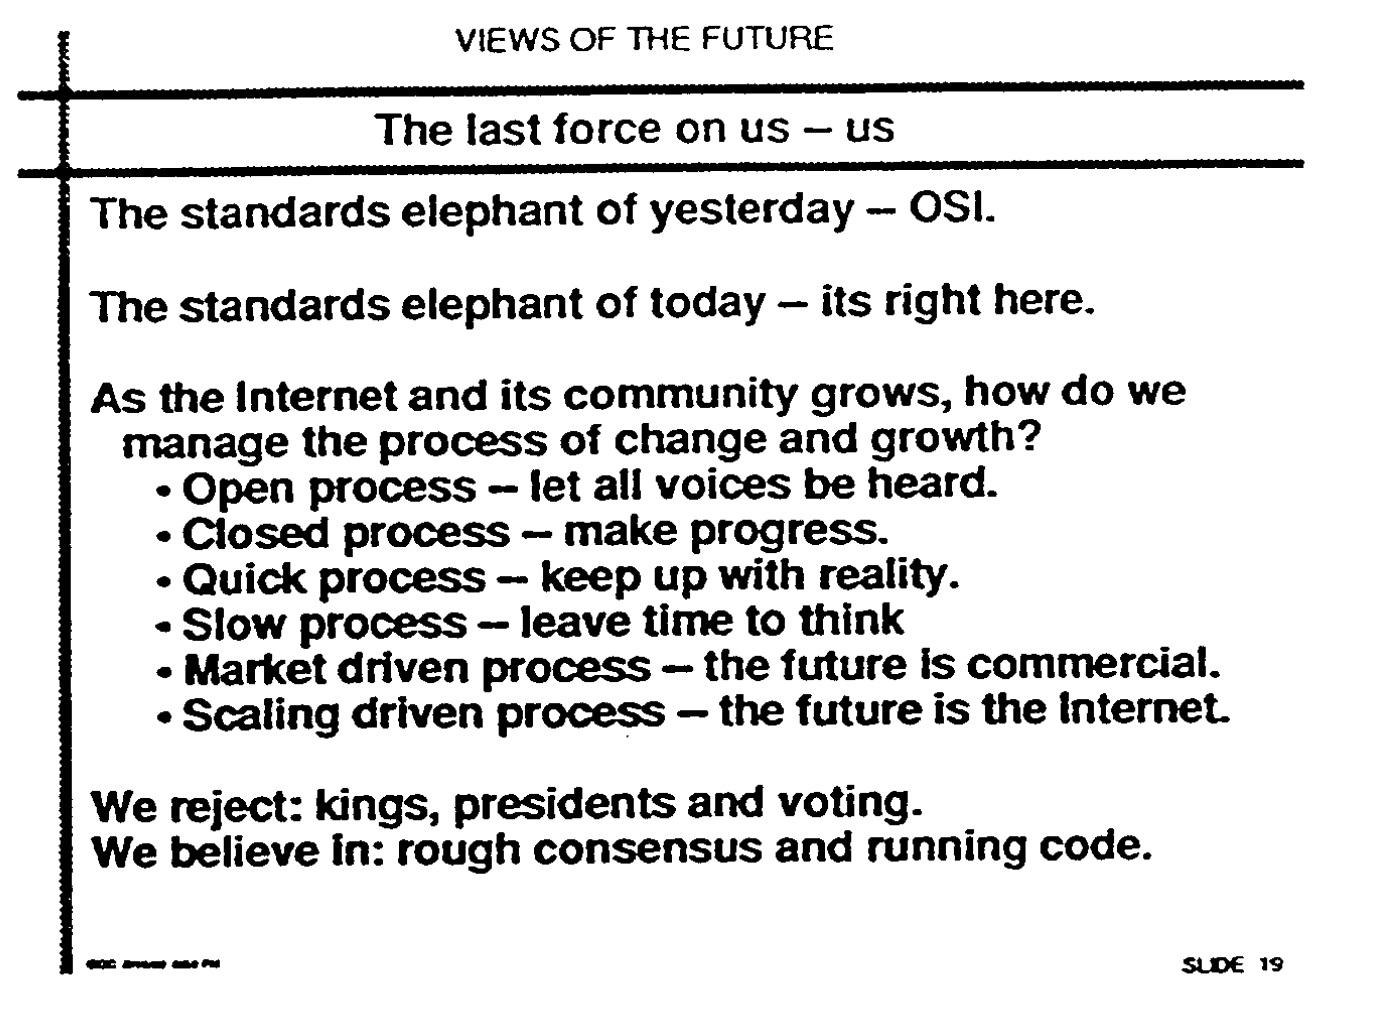
\includegraphics[width=\linewidth]{../assets/images/clark-slide.png} \emph{A
slide from David Clark's ``Views of the Future''\cite{clarkCloudyCrystalBall1992}  that contrasts differing visions for the
development process of the future of the internet. The struggle between
engineered order and wild untamedness is summarized forcefully as ``We
reject: kings, presidents and voting. We believe in: rough consensus and
running code}

Practically, the differences between these thought communities impact
the tools they build. Aaron Swartz put the approach of the ``neat''
semantic web architects the way he did:

\begin{quote}
Instead of the ``let's just build something that works'' attitude that
made the Web (and the Internet) such a roaring success, they brought the
formalizing mindset of mathematicians and the institutional structures
of academics and defense contractors. They formed committees to form
working groups to write drafts of ontologies that carefully listed (in
100-page Word documents) all possible things in the universe and the
various properties they could have, and they spent hours in Talmudic
debates over whether a washing machine was a kitchen appliance or a
household cleaning device.

With them has come academic research and government grants and corporate
R\&D and the whole apparatus of people and institutions that scream
``pipedream.'' And instead of spending time building things, they've
convinced people interested in these ideas that the first thing we need
to do is write standards. (To engineers, this is absurd from the
start---standards are things you write after you've got something
working, not before!) \cite{swartzAaronSwartzProgrammable2013} 
\end{quote}

The outcomes of this cultural rift are subtle, but the broad strokes are
clear: the ``scruffies'' largely diverged into the linked data
community, which has taken some of the core semantic web technology like
RDF, OWL, and the like, and developed a broad range of downstream
technologies that have found purchase across information sciences,
library sciences, and other applied domains\footnote{This isn't a story
  of ``good people'' and ``bad people,'' as a lot of the linked data
  technology also serves as the backbone for abusive technology
  monopolies like google's acquisition of Freebase \cite{iainFreebaseDeadLong2019}  and the profusion of knowledge
  graph-based medical platforms.}. The linked data developers, starting
by acknowledging that no one system can possibly capture everything,
build tools that allow expression of local systems of meaning with the
expectation and affordances for linking data between these systems as an
ongoing social process.

The vision of a totalizing and logically consistent semantic web,
however, has largely faded into obscurity. One developer involved with
semantic web technologies (who requested not be named), captured the
present situation in their description of a still-active developer
mailing list:

\begin{quote}
I think that some people are completely detached from practical
applications of what they propose. {[}\ldots{]} I could not follow half
of the messages. these guys seem completely removed from our plane of
existence and I have no clue what they are trying to solve.
\end{quote}

This division in thought styles generalizes across domains of
infrastructure, though outside of the linked data and similar worlds the
dichotomy is more frequently between ``neatness'' and ``people doing
whatever'' -- with integration and interoperability becoming nearly
synonymous with standardization. Calls for standardization without
careful consideration and incorporation of existing practice have a
familiar cycle: devise a standard that will solve everything, implement
it, wonder why people aren't using it, funding and energy dissipiates,
rinse, repeat. The difficulty of scaling an exacting vision of how data
should be formatted, the tools researchers should use for their
experiments, and so on is that they require dramatic and sometimes total
changes to the way people do science. The alternative is not between
standardization and chaos, but a potential third way is designing
infrastructures that allow the diversity of approaches, tools, and
techniques to be expressed in a common framework or protocol along with
the community infrastructure to allow the continual negotiation of their
relationship.

\hypertarget{taped-on-interfaces-open-loop-user-testing}{%
\subsubsection{Taped-on Interfaces: Open-Loop User
Testing}\label{taped-on-interfaces-open-loop-user-testing}}

The point of most active competition in many domains of commercial
software is the user interface and experience (UI/UX), and to compete
software companies will exhaustively user-test and refine them with
pixel precision to avoid any potential customer feeling even a
thimbleful of frustration. Scientific software development is largely
disconnected from usability testing, as what little support exists is
rarely tied to it. This, combined with the above incentives for
developing new packages -- and thus reduplicating the work of interface
development -- and the preponderance of semi-amateurs make it perhaps
unsurprising that most scientific software is hard to use!

I intend the notion of ``interface'' in an expansive way: In addition to
the graphical user interface (GUI) exposed to the end-user, I am
referring generally to all points of contact with users, developers, and
other software. Interfaces are intrinsically social, and include the
surrounding documentation and experience of use --- part of using an API
is being able to figure out how to use it! The typical form of
scientific software is a black box: I implemented an algorithm of some
kind, here is how to use it, but beneath the surface there be dragons.

Ideally, software would be designed with programming interfaces and
documentation at multiple scales of complexity to enable clean
entrypoints for developers with differing levels of skill and investment
to contribute. Additionally, it would include interfaces for use and
integration with other software. Without care given to either of these
interfaces, the community of co-developers is likely to remain small,
and the labor they expend is less likely to be useful outside that
single project. This, in turn, reinforces the incentives for developing
new packages and fragmentation.

\hypertarget{platforms-industry-capture-and-the-profit-motive}{%
\subsubsection{Platforms, Industry Capture, and the Profit
Motive}\label{platforms-industry-capture-and-the-profit-motive}}

Publicly funded science is an always-irresistable golden goose for
private industry. The fragmented interests of scientists and the
historically light touch of funding agencies on encroaching
privatization means that if some company manages to capture and
privatize a corner of scientific practice they are likely to keep it.
Industry capture has been thoroughly criticized in the context of the
journal system (eg. recently, \cite{brembsReplacingAcademicJournals2021} ), and that criticism should
extend to the rest of our infrastructure as information companies seek
to build a for-profit platform system that spans the scientific workflow
(eg. \cite{ElsevierSevenBridges2017} ). The mode of privatization
of scientific infrastructure follows the broader software market as a
preponderance of software as a service (SaaS), from startups to
international megacorporations, that sell access to some, typically
proprietary software without selling the software itself.

While in isolation SaaS can make individual components of the
infrastructural landscape easier to access --- and even free!!* --- the
business model is fundamentally incompatible with integrated and
accessible infrastructure. The SaaS model derives revenue from
subscription or use costs, often operating as ``freemium'' models that
make some subset of its services available for free. Even in freemium
models, though, the business model requires that some functionality of
the platform is paywalled (See a more thorough treatment of platform
capitalism in science in \cite{mirowskiFutureOpenScience2018} )

As isolated services, one can imagine the practice of science devolving
along a similar path as the increasingly-fragmented streaming video
market: to do my work I need to subscribe to a data storage service, a
cloud computing service, a platform to host my experiments, etc. For
larger software platforms, however, vertical integration of multiple
complementary services makes their impact on infrastructure more
insidious. Locking users into more and more services makes for more and
more revenue, which encourages platforms to be as mutually incompatible
as they can get away with \cite{macinnesCompatibilityStandardsMonopoly2005} . To encourage adoption,
platforms that can offer multiple services may offer one of the services
-- say, data storage -- for free, forcing the user to use the adjoining
services -- say, a cloud computing platform.

Since these platforms are often subsidiaries of information industry
monopolists, scientists become complicit in their often profoundly
unethical behavior of by funneling millions of dollars into them.
Longterm, unconditional funding of wildly profitable journals has
allowed conglomerates like Elsevier to become sprawling surveillance
companies \cite{RELXAnnualReport2020}  that are sucking as much
data up as they can to market tools like algorithmic ranking of
scientific productivity \cite{brembsAlgorithmicEmploymentDecisions2021}  and making data sharing
agreements with ICE \cite{biddleLexisNexisProvideGiant2021} . Or
see our use of AWS and the laundry list of human rights abuses by Amazon
\cite{CriticismAmazon2021} . In addition to lock-in, dependence
on a constellation of SaaS allows the opportunity for platform-holders
to take advantage of their limitations and \emph{sell us additional
services to make up for what the other ones purposely lack} --- for
example Elsevier has taken advantage of our dependence on the journal
system and its strategic disorganization to sell a tool for summarizing
trending research areas for tailoring maximally-fundable grants \cite{elsevierTopicProminenceSciencea} .

Funding models and incentive structures in science are uniformly aligned
towards the platformatization of scientific infrastructure. Aside from
the corporate doublespeak rhetoric of ``technology transfer'' that
pervades the neoliberal university, the relative absence of major
funding opportunities for scientific software developers competitive
with the profit potential from ``industry'' often leaves it as the only
viable career path. The preceding structural constraints on local
infrastructural development strongly incentivize labs and researchers to
rely on SaaS that provides a readymade solution to specific problems.
Distressingly, rather than supporting infrastructural development that
would avoid obligate payments to platform-holders, funding agencies seem
all too happy to lean into them (emphases mine):

\begin{quote}
NIH will \textbf{leverage what is available in the private sector,}
either through strategic partnerships or procurement, to create a
workable \textbf{Platform as a Service (PaaS)} environment. {[}\ldots{]}
NIH will partner with cloud-service providers for cloud storage,
computational, and related infrastructure services needed to facilitate
the deposit, storage, and access to large, high-value NIH datasets.
{[}\ldots{]}

NIH's cloud-marketplace initiative will be the first step in a phased
operational framework that \textbf{establishes a SaaS paradigm for NIH
and its stakeholders.} (-NIH Strategic Plan for Data Science, 2018 \cite{NIHStrategicPlan2018} )
\end{quote}

The articulated plan being to pay platform holders to house data while
also paying for the labor to maintain those databases veers into parody,
haplessly building another triple-pay industry \cite{buranyiStaggeringlyProfitableBusiness2017}  into the economic system
of science --- one can hardly wait until they have the opportunity to
rent their own data back with a monthly subscription. This isn't a
metaphor: the STRIDES program, with the official subdomain
\href{https://web.archive.org/web/20210729131920/https://cloud.nih.gov/}{cloud.nih.gov},
has been authorized to pay \$85 million to cloud providers since 2018.
In exchange, NIH hasn't received any sort of new technology, but
\href{https://web.archive.org/web/20211006003547/https://cloud.nih.gov/enrollment/account-type/}{``extramural''}
scientists receive a maximum discount of 25\% on cloud storage and
``data egress'' fees as well as plenty of training on how to give
control of the scientific process to platform giants \cite{reillyNIHSTRIDESInitiative2021} \footnote{Their success stories tell
  the story of platform non-integration where scientists have to
  handbuild new tools to manage their data across multiple cloud
  environments: ``We have been storing data in both cloud environments
  because we wanted the ecosystem we are creating to work on both
  clouds'' \cite{STRIDESInitiativeSuccess2020} }. With platforms,
without exaggeration we pay them to let us pay for something that makes
it so we need to pay them more later.

It is unclear to me whether this is the result of the cultural hegemony
of platform capitalism narrowing the space of imaginable
infrastructures, industry capture of the decision-making process, or
both, but the effect is the same in any case.

\hypertarget{protection-of-institutional-and-economic-power}{%
\subsubsection{Protection of Institutional and Economic
Power}\label{protection-of-institutional-and-economic-power}}

Aside from information industries, infrastructural deficits are
certainly not without beneficiaries within science --- those that have
already accrued power and status.

Structurally, the adoption of SaaS on a wide scale necessarily
sacrifices the goals of an integrated mass infrastructure as the
practice of research is carved into small, marketable chunks within
vertically integrated technology platforms. Worse, it stands to amplify,
rather than reduce, inequities in science, as the labs and institutes
that are able to afford the tolls between each of the weigh stations of
infrastructure are able to operate more efficiently --- one of many
positive feedback loops of inequity.

More generally, incentives across infrastructures are often misaligned
across strata of power and wealth. Those at the top of a power hierarchy
have every incentive to maintain the fragmentation that prevents people
from competing --- hopefully mostly unconsciously via uncritically
participating in the system rather than maliciously reinforcing it.

This poses an organizational problem: the kind of infrastructure that
unwinds platform ownership is not only unprofitable, it's
anti-profitable -- making it impossible to profit from its domain of
use. That makes it difficult to rally the kind of development and
\href{https://www.snsi.info/}{lobbying} resources that profitable
technology can, requiring organization based on ethical principles and a
commitment to sacrifice control in order to serve a practical need.

The problem is not insurmountable, and there are strategic advantages to
decentralized infrastructure and its development within science.
Centralized technologies and companies might have more concerted power,
but we have \emph{numbers} and can make tools that allow us to combine
small amounts of labor from many people. A primary criticism of
infrastructural overhauls is that they will cost a lot of \emph{money,}
but that's propaganda: the cost of decentralized technologies is far
smaller than the vast sums of money funnelled into industry profits,
labor hours spent compensating for the designed inefficiencies of the
platform model, and the development of a fragmented tool ecosystem built
around them.

Science, as one of few domains of non-economic labor, has the
opportunity to be a seed for decentralized technologies that could
broadly improve not only the health of scientific practice, but the
broader information ecosystem. If we develop a plan and mobilize to make
use of our collective expertise to build tools that have no business
model and no means of development in commercial domains --- we just need
to realize what's at stake, develop a plan, and agree that the health of
science is more important than the convenience of the cloud or which
journal our papers go into. 
\end{multicols}


\hypertarget{the-ivies-institutes-and-the-rest-of-us}{%
\subsection{The Ivies, Institutes, and ``The Rest of
Us''}\label{the-ivies-institutes-and-the-rest-of-us}}


\begin{multicols}{2}
 Given these constraints These constraints manifest
differently depending on the circumstance of scientific practice.
Differences in circumstance of practices also influence the kind of
infrastructure developed, as well as where we should expect
infrastructure development to happen as well as who benefits from it.

\hypertarget{institutional-core-facilities}{%
\subsubsection{Institutional Core
Facilities}\label{institutional-core-facilities}}

Centralized ``core'' facilities are maybe the most typical form of
infrastructure development and resource sharing at the level of
departments and institutions. These facilities can range from minimal to
baroque extravagance depending on institutional resources and whatever
complex web of local history brought them about.

\href{https://projectreporter.nih.gov/project_info_details.cfm?aid=9444124}{PNI
Systems Core} lists
\href{https://reporter.nih.gov/project-details/9444124\#sub-Projects}{subprojects}
echo a lot of the thoughts here, particularly around effort
duplication\footnote{Thanks a lot to the one-and-only stunning and
  brilliant Dr.~Eartha Mae Guthman for suggesting looking at the BRAIN
  initiative grants as a way of getting insight on core facilities.}:

\begin{quote}
Creating an Optical Instrumentation Core will address the problem that
much of the technical work required to innovate and maintain these
instruments has shifted to students and postdocs, because it has
exceeded the capacity of existing staff. This division of labor is a
problem for four reasons: (1) lab personnel often do not have sufficient
time or expertise to produce the best possible results, (2) the
diffusion of responsibility leads people to duplicate one another's
efforts, (3) researchers spend their time on technical work at the
expense of doing science, and (4) expertise can be lost as students and
postdocs move on. For all these reasons, we propose to standardize this
function across projects to improve quality control and efficiency.
Centralizing the design, construction, maintenance, and support of these
instruments will increase the efficiency and rigor of our microscopy
experiments, while freeing lab personnel to focus on designing
experiments and collecting data.
\end{quote}

While core facilities are an excellent way of expanding access, reducing
redundancy, and standardizing tools within an instutition, as commonly
structured they can displace work spent on those efforts outside of the
institution. Elite institutions can attract the researchers with the
technical knowledge to develop the instrumentation of the core and
infrastructure for maintain it, but this development is only
occasionally made usable by the broader public. The Princeton data
science core is an excellent example of a core facility that does makes
its software infrastructure development
\href{https://github.com/BrainCOGS}{public}\footnote{\begin{quote}
  Project Summary: Core 2, Data Science {[}\ldots{]} In addition, the
  Core will build a data science platform that stores behavior, neural
  activity, and neural connectivity in a relational database that is
  queried by the DataJoint language. {[}\ldots{]} This data-science
  platform will facilitate collaborative analysis of datasets by
  multiple researchers within the project, and make the analyses
  reproducible and extensible by other researchers. {[}\ldots{]}
  https://projectreporter.nih.gov/project\_info\_description.cfm?aid=9444126\&icde=0
  \end{quote}}, which they should be applauded for, but also
illustrative of the problems with a core-focused infrastructure project.
For an external user, the documentation and tutorials are incomplete --
it's not clear to me how I would set this up for my institute, lab, or
data, and there are several places of hard-coded princeton-specific
values that I am unsure how exactly to adapt\footnote{Though again, this
  project is examplary, built by friends, and would be an excellent
  place to start extending towards global infrastructure.}. I would
consider this example a high-water mark, and the median openness of core
infrastructure falls far below it. I was unable to find an example of a
core facility that maintained publicly-accessible documentation on the
construction and operation of its experimental infrastructure or the
management of its facility.

\hypertarget{centralized-institutes}{%
\subsubsection{Centralized Institutes}\label{centralized-institutes}}

Outside of universities, the Allen Brain Institute is perhaps the most
impactful reflection of centralization in neuroscience. The Allen
Institute has, in an impressively short period of time, created several
transformative tools and datasets, including its well-known atlases \cite{leinGenomewideAtlasGene2007}  and the first iteration of its
\href{http://observatory.brain-map.org/}{Observatory} project which
makes a massive, high-quality calcium imaging dataset of visual cortical
activity available for public use. They also develop and maintain
software tools like their
\href{https://allensdk.readthedocs.io/en/latest/}{SDK} and Brain
Modeling Toolkit \href{https://alleninstitute.github.io/bmtk/}{(BMTK)},
as well as a collection of
\href{https://portal.brain-map.org/explore/toolkit/hardware}{hardware
schematics} used in their experiments. The contribution of the Allen
Institute to basic neuroscientific infrastructure is so great that,
anecdotally, when talking about scientific infrastructure it's not
uncommon for me to hear something along the lines of ``I thought the
Allen was doing that.''

Though the Allen Institute is an excellent model for scale at the level
of a single organization, its centralized, hierarchical structure cannot
(and does not attempt to) serve as the backbone for all neuroscientific
infrastructure. Performing single (or a small number of, as in its
also-admirable
\href{https://alleninstitute.org/what-we-do/brain-science/news-press/articles/three-collaborative-studies-launch-openscope-shared-observatory-neuroscience}{OpenScope
Project}) carefully controlled experiments a huge number of times is an
important means of studying constrained problems, but is complementary
with the diversity of research questions, model organisms, and methods
present in the broader neuroscientific community.

Christof Koch, its director, describes the challenge of centrally
organizing a large number of researchers:

\begin{quote}
Our biggest institutional challenge is organizational: assembling,
managing, enabling and motivating large teams of diverse scientists,
engineers and technicians to operate in a highly synergistic manner in
pursuit of a few basic science goals \cite{grillnerWorldwideInitiativesAdvance2016} 
\end{quote}

\begin{quote}
These challenges grow as the size of the team grows. Our anecdotal
evidence suggests that above a hundred members, group cohesion appears
to become weaker with the appearance of semi-autonomous cliques and
sub-groups. This may relate to the postulated limit on the number of
meaningful social interactions humans can sustain given the size of
their brain \cite{kochBigScienceTeam2016} 
\end{quote}

!! These institutes are certainly helpful in building core technologies
for the field, but they aren't necessarily organized for developing
mass-scale infrastructure.

\hypertarget{meso-scale-collaborations}{%
\subsubsection{Meso-scale
collaborations}\label{meso-scale-collaborations}}

Given the diminishing returns to scale for centralized organizations,
many have called for smaller, ``meso-scale'' collaborations and
consortia that combine the efforts of multiple labs \cite{mainenBetterWayCrack2016} . The most successful consortium of this
kind has been the International Brain Laboratory \cite{abbottInternationalLaboratorySystems2017, woolKnowledgeNetworksHow2020} , a group of 22 labs spread across six countries. They have been
able to realize the promise of big team neuroscience, setting a new
standard for performing reproducible experiments performed by many labs
\cite{laboratoryStandardizedReproducibleMeasurement2020}  and
developing data management infrastructure to match \cite{laboratoryDataArchitectureLargescale2020}  (seriously, don't miss
their extremely impressive
\href{https://data.internationalbrainlab.org/}{data portal}). Their
project thus serves as the benchmark for large-scale collaboration and a
model from which all similar efforts should learn from.

Critical to the IBL's success was its adoption of a flat,
non-hierarchical organizational structure, as described by Lauren E.
Wool:

\begin{quote}
IBL's virtual environment has grown to accommodate a diversity of
scientific activity, and is supported by a flexible, `flattened'
hierarchy that emphasizes horizontal relationships over vertical
management. {[}\ldots{]} Small teams of IBL members collaborate on
projects in Working Groups (WGs), which are defined around particular
specializations and milestones and coordinated jointly by a chair and
associate chair (typically a PI and researcher, respectively). All WG
chairs sit on the Executive Board to propagate decisions across WGs,
facilitate operational and financial support, and prepare proposals for
voting by the General Assembly, which represents all PIs. \cite{woolKnowledgeNetworksHow2020} 
\end{quote}

They should also be credited with their adoption of a form of consensus
decision-making, \href{https://sociocracy.info}{sociocracy}, rather than
a majority-vote or top-down decisionmaking structure. Consensus
decision-making systems are derived from those developed by
\href{https://rhizomenetwork.wordpress.com/2011/06/18/a-brief-history-of-consenus-decision-making/}{Quakers
and some Native American nations}, and emphasize, perhaps
unsurprisingly, the value of collective consent rather than the will of
the majority.

The central lesson of the IBL, in my opinion, is that governance
matters. Even if a consortium of labs were to form on an ad-hoc basis,
without a formal system to ensure contributors felt heard and empowered
to shape the project it would soon become unsustainable. Even if this
system is not perfect, with some labor still falling unequally on some
researchers, it is a promising model for future collaborative consortia.

The infrastructure developed by the IBL is impressive, but its focus on
a single experiment makes it difficult to expand and translate to
widescale use. The hardware for the IBL experimental apparatus is
exceptionally well-documented, with a
\href{https://figshare.com/articles/preprint/A_standardized_and_reproducible_method_to_measure_decision-making_in_mice_Appendix_3_IBL_protocol_for_setting_up_the_behavioral_training_rig/11634732}{complete
and detailed build guide} and
\href{https://figshare.com/articles/online_resource/A_standardized_and_reproducible_method_to_measure_decision-making_in_mice_CAD_files_for_behavior_rig/11639973}{library
of CAD parts}, but the documentation is not modularized such that it
might facilitate use in other projects, remixed, or repurposed. The
\href{https://github.com/int-brain-lab/iblrig}{experimental software} is
similarly single-purpose, a chimeric combination of Bonsai \cite{lopesBonsaiEventbasedFramework2015}  and
\href{https://github.com/pybpod/pybpod}{PyBpod}
\href{https://github.com/int-brain-lab/iblrig/tree/master/tasks/_iblrig_tasks_ephysChoiceWorld}{scripts}.
It unfortunately
\href{https://iblrig.readthedocs.io/en/latest/index.html}{lacks} the
API-level documentation that would facilitate use and modification by
other developers, so it is unclear to me, for example, how I would use
the experimental apparatus in a different task with perhaps slightly
different hardware, or how I would then contribute that back to the
library. The experimental software, according to the
\href{https://figshare.com/articles/preprint/A_standardized_and_reproducible_method_to_measure_decision-making_in_mice_Appendix_3_IBL_protocol_for_setting_up_the_behavioral_training_rig/11634732}{PDF
documentation}, will also not work without a connection to an
\href{https://github.com/cortex-lab/alyx}{alyx} database. While alyx was
intended for use outside the IBL, it still has
\href{https://github.com/cortex-lab/alyx/blob/07f481f6bbde668b81ad2634f4c42df4d6a74e44/alyx/data/management/commands/files.py\#L188}{IBL-specific}
and
\href{https://github.com/cortex-lab/alyx/blob/07f481f6bbde668b81ad2634f4c42df4d6a74e44/alyx/data/fixtures/data.datasettype.json\#L29}{task-specific}
values in its source-code, and makes community development difficult
with a similar \href{https://alyx.readthedocs.io/en/latest/}{lack} of
API-level documentation and requirement that users edit the library
itself, rather than temporary user files, in order to use it outside the
IBL.

My intention is not to denigrate the excellent tools built by the IBL,
nor their inspiring realization of meso-scale collaboration, but to
illustrate a problem that I see as an extension of that discussed in the
context of core facilities --- designing infrastructure for one task, or
one group in particular makes it much less likely to be portable to
other tasks and groups.

It is also unclear how replicable these consortia are, and whether they
challenge, rather than reinforce technical inequity in science.
Participating in consortia systems like the IBL requires that labs have
additional funding for labor hours spent on work for the consortium, and
in the case of graduate students and postdocs, that time can conflict
with work on their degrees or personal research which are still far more
potent instruments of ``remaining employed in science'' than
collaboration. In the case that only the most well-funded labs and
institutions realize the benefits of big team science without explicit
consideration given to scientific equity, mesoscale collaborations could
have the unintended consequence of magnifying the skewed distribution of
access to technical expertise and instrumentation.

\hypertarget{the-rest-of-us}{%
\subsubsection{The rest of us\ldots{}}\label{the-rest-of-us}}

Outside of ivies with rich core facilities, institutes like the Allen,
or nascent multi-lab consortia, the rest of us are largely on our own,
piecing together what we can from proprietary and open source
technology. The world of open source scientific software has plenty of
energy and lots of excellent work is always being done, though
constrained by the circumstances of its development described briefly
above. Anything else comes down to whatever we can afford with remaining
grant money, scrape together from local knowledge, methods sections,
begging, borrowing, and (hopefully not too much) stealing from
neighboring labs.

A third option from the standardization offered by centralization and
the blooming, buzzing, beautiful chaos of disconnected open-source
development is that of decentralized systems, and with them we might
build the means by which the ``rest of us'' can mutually benefit by
capturing and making use of each other's knowledge and labor.

\end{multicols}


\hypertarget{a-draft-of-decentralized-scientific-infrastructure}{%
\section{A Draft of Decentralized Scientific
Infrastructure}\label{a-draft-of-decentralized-scientific-infrastructure}}


\begin{multicols}{2}
 Where do we go from here?

The decentralized infrastructure I will describe here is similar to
previous notions of ``grass-roots'' science articulated within systems
neuroscience \cite{mainenBetterWayCrack2016}  but has broad and
deep history in many domains of computing. My intention is to provide a
more prescriptive scaffolding for its design and potential
implementation as a way of painting a picture of what science could be
like. This sketch is not intended to be final, but a starting point for
further negotiation and refinement.

Throughout this section, when I am referring to any particular piece of
software I want to be clear that I don't intend to be dogmatically
advocating that software \emph{in particular}, but software \emph{like
it} that \emph{shares its qualities} --- no snake oil is sold in this
document. Similarly, when I describe limitations of existing tools,
without exception I am describing a tool or platform I love, have
learned from, and think is valuable --- learning from something can mean
drawing respectful contrast!

\hypertarget{design-principles}{%
\subsection{Design Principles}\label{design-principles}}

I won't attempt to derive a definition of decentralized systems from
base principles here, but from the systemic constraints described above,
some design principles that illustrate the idea emerge naturally. For
the sake of concrete illustration, in some of these I will additionally
draw from the architectural principles of the internet protocols: the
most successful decentralized digital technology project.

!! need to integrate \cite{larsenPoliticalNatureTCP2012} 

\{\% include rdfa.html id=``protocols'' resource=``protocols''
typeof=``skos:Concept'' contents=``\#\#\# Protocols, not Platforms''
\%\}

Much of the basic technology of the internet was developed as
\emph{protocols} that describe the basic attributes and operations of a
process. \{\% include rdfa2.html resource=``protocols''
property=``skos:example'' contents=``A simple and common example is
email over SMTP (Simple Mail Transfer Protocol)'' \%\} \cite{Rfc5321SimpleMail} . SMTP describes a series of steps that email
servers must follow to send a message: the sender initiates a connection
to the recipient server, the recipient server acknowledges the
connection, a few more handshake steps ensue to describe the senders and
receivers of the message, and then the data of the message is
transferred. Any software that implements the protocol can send and and
receive emails to and from any other. The protocol basis of email is the
reason why it is possible to send an email from a gmail account to a
hotmail account (or any other hacky homebrew SMTP client) despite being
wholly different pieces of software.

In contrast, \emph{platforms} provide some service with a specific body
of code usually without any pretense of generality. In contrast to email
over SMTP, we have grown accustomed to not being able to send a message
to someone using Telegram from WhatsApp, switching between multiple
mutually incompatible apps that serve nearly identical purposes.
Platforms, despite being \emph{theoretically} more limited than
associated protocols, are attractive for many reasons: they provide
funding and administrative agencies a single point of contracting and
liability, they typically provide a much more polished user interface,
and so on. These benefits are short-lived, however, as the inevitable
toll of lock-in and shadowy business models is realized.

\hypertarget{integration-not-invention}{%
\subsubsection{Integration, not
Invention}\label{integration-not-invention}}

At the advent of the internet protocols, several different institutions
and universities had already developed existing network infrastructures,
and so the ``top level goal'' of IP was to ``develop an effective
technique for multiplex utilization of existing interconnected
networks,'' and ``come to grips with the problem of integrating a number
of separately administered entities into a common utility'' \cite{clarkDesignPhilosophyDARPA1988} . As a result, IP was developed as a
`common language' that could be implemented on any hardware, and upon
which other, more complex tools could be built. This is also a cultural
practice: when the system doesn't meet some need, one should try to
extend it rather than building a new, separate system --- and if a new
system is needed, it should be interoperable with those that exist.

This point is practical as well as tactical: to compete, an emerging
protocol should integrate or be capable of bridging with the
technologies that currently fill its role. A new database protocol
should be capable of reading and writing existing databases, a new
format should be able to ingest and export to existing formats, and so
on. The degree to which switching is seamless is the degree to which
people will be willing to switch.

This principle runs directly contrary to the current incentives for
novelty and fragmentation, which must be directly counterbalanced by
design choices elsewhere to address the incentives driving them.

\hypertarget{embrace-heterogeneity-be-uncoercive}{%
\subsubsection{Embrace Heterogeneity, Be
Uncoercive}\label{embrace-heterogeneity-be-uncoercive}}

A reciprocal principle to integration with existing systems is to design
the system to be integratable with existing practice. Decentralized
systems need to anticipate unanticipated uses, and can't rely on
potential users making dramatic changes to their existing practices. For
example, an experimental framework should not insist on a prescribed set
of supported hardware and rigid formulation for describing experiments.
Instead it should provide affordances that give a clear way for users to
extend the system to fit their needs \cite{carpenterRFC1958Architectural1996} . In addition to integrating with
existing systems, it must be straightforward for future development to
be integrated. This idea is related to ``the test of independent
invention'', summarized with the question ``if someone else had already
invented your system, would theirs work with yours?'' \cite{berners-leePrinciplesDesign1998} .

This principle also has tactical elements. An uncoercive system allows
users to gradually adopt it rather than needing to adopt all of its
components in order for any one of them to be useful. There always needs
to be a \emph{benefit} to adopting further components of the system to
encourage \emph{voluntary} adoption, but it should never be
\emph{compulsory.} For example, again from experimental frameworks, it
should be possible to use it to control experimental hardware without
needing to use the rest of the experimental design, data storage, and
interface system. To some degree this is accomplished with a modular
system design where designers are mindful of keeping the individual
modules independently useful.

A noncoercive architecture also prioritizes the ease of leaving. Though
this is somewhat tautological to protocol-driven design, specific care
must be taken to enable export and migration to new systems. Making
leaving easy also ensures that early missteps in development of the
system are not fatal to its development, preventing lock-in to a
component that needs to be restructured.

!! the coercion of centralization has a few forms. this is related to
the authoritarian impulse in the open science movement that for awhile
bullied people into openness. that instinct in part comes from a belief
that everyone should be doing the same thing, should be posting their
work on the one system. decentralization is about autonomy, and so a
reciprocal approach is to make it easy and automatic.

\hypertarget{empower-people-not-systems}{%
\subsubsection{Empower People, not
Systems}\label{empower-people-not-systems}}

Because IP was initially developed as a military technology by DARPA, a
primary design constraint was survivability in the face of failure. The
model adopted by internet architects was to move as much functionality
from the network itself to the end-users of the network --- rather than
the network itself guaranteeing a packet is transmitted, the sending
computer will do so by requiring a response from the recipient \cite{clarkDesignPhilosophyDARPA1988} .

For infrastructure, we should make tools that don't require a central
team of developers to maintain, a central server-farm to host data, or a
small group of people to govern. Whenever possible, data, software, and
hardware should be self-describing, so one needs minimal additional
tools or resources to understand and use it. It should never be the case
that funding drying up for one node in the system causes the entire
system to fail.

Practically, this means that the tools of digital infrastructure should
be deployable by individual people and be capable of recapitulating the
function of the system without reference to any central authority.
Researchers need to be given control over the function of
infrastructure: from controlling sharing permissions for eg. clinically
sensitive data to assurance that their tools aren't spying on them.
Formats and standards must be negotiable by the users of a system rather
than regulated by a central governance body.

\hypertarget{infrastructure-is-social}{%
\subsubsection{Infrastructure is
Social}\label{infrastructure-is-social}}

The alternative to centralized governing and development bodies is to
build the tools for community control over infrastructural components.
This is perhaps the largest missing piece in current scientific tooling.
On one side, decentralized governance is the means by which an
infrastructure can be maintained to serve the ever-evolving needs of its
users. On the other, a sense of community ownership is what drives
people to not only adopt but contribute to the development of an
infrastructure. In addition to a potentially woo-woo sense of socially
affiliative ``community-ness,'' any collaborative system needs a way of
ensuring that the practice of maintaining, building, and using it is
designed to \emph{visibly and tangibly benefit} those that do, rather
than be relegated to a cabal of invisible developers and maintainers
\cite{grudinGroupwareSocialDynamics1994, randallDistributedOntologyBuilding2011} .

Governance and communication tools also make it possible to realize the
infinite variation in application that infrastructures need while
keeping them coherent: tools must be built with means of bringing the
endless local conversations and modifications of use into a common space
where they can become a cumulative sense of shared memory.

This idea will be given further treatment and instantiation in a later
discussion of the social dynamics of private bittorrent trackers, and is
necessarily diffuse because of the desire to not be authoritarian about
the structure of governance.

\hypertarget{usability-matters}{%
\subsubsection{Usability Matters}\label{usability-matters}}

It is not enough to build a technically correct technology and assume it
will be adopted or even useful, it must be developed embedded within
communities of practice and \emph{be useful for solving problems that
people actually have.} We should learn from the struggles of the
semantic web project. Rather than building a fully prescriptive and
complete system first and instantiating it later, we should develop
tools whose usability is continuously improved \emph{en route} to a
(flexible) completed vision.

The adage from RFC 1958 ``nothing gets standardized until there are
multiple instances of running code'' \cite{carpenterRFC1958Architectural1996}  captures the dual nature of the
constraint well. Workable standards don't emerge until they have been
extensively tested in the field, but development without an eye to an
eventual protocol won't make one.

We should read the
\href{https://en.wikipedia.org/wiki/Embrace,_extend,_and_extinguish}{gobbling
up} of open protocols into proprietary platforms that defined ``Web
2.0'' as instructive (in addition to a demonstration of the raw power of
concentrated capital) \cite{markoffTomorrowWorldWide1996} .
\emph{Why} did Slack outcompete IRC? The answer is relatively simple: it
was relatively simple to use. Using a contemporary example, to
\href{https://matrix-org.github.io/synapse/latest/setup/installation.html}{set
up a Synapse server} to communicate over
\href{https://matrix.org/docs/spec/}{Matrix} one has to wade through
dozens of shell commands, system-specific instructions, potential
conflicts between dependent packages, set up an SQL server\ldots{} and
that's just the backend, we don't even have a frontend client yet! In
contrast, to use Slack you download the app, give it your email, and
you're off and running.

The control exerted by centralized systems over their system design does
give certain structural advantages to their usability, and their
for-profit model gives certain advantages to their development process.
There is no reason, however, that decentralized systems \emph{must} be
intrinsically harder to use, we just need to focus on user experience to
a comparable degree that centralized platforms: if it takes a college
degree to turn the water on, that ain't infrastructure.

People are smart, they just get frustrated easily. We have to raise our
standards of design such that we don't expect users to have even a
passing familiarity with programming, attempting to build tools that are
truly general use. We can't just design a peer-to-peer system, we need
to make the data ingestion and annotation process automatic and
effortless. We can't just build a system for credit assignment, it needs
to happen as an automatic byproduct of using the system. We can't just
make tools that \emph{work,} they need to \emph{feel good to use.}

Centralized systems also have intrinsic limitations that provide
openings for decentralized systems, like cost, incompatibility with
other systems, inability for extension, and opacity of function. The
potential for decentralized systems to capture the independent
development labor of all of its users, rather than just that of a core
development team, is one means of competition. If the barriers to
adoption can be lowered, and the benefits raised these constant negative
pressures of centralization might overwhelm intertia.

With these principles in mind, and drawing from other knowledge
communities solving similar problems: internet infrastructure,
library/information science, peer-to-peer networks, and radical
community organizers, I conceptualize a system of distributed
infrastructure for systems neuroscience as three objectives:
\protect\hyperlink{shared-data}{\textbf{shared data}},
\protect\hyperlink{shared-tools}{\textbf{shared tools}}, and
\protect\hyperlink{shared-knowledge}{\textbf{shared knowledge}}.

\end{multicols}


\hypertarget{shared-data}{%
\subsection{Shared Data}\label{shared-data}}

\hypertarget{formats-as-onramps}{%
\subsubsection{Formats as Onramps}\label{formats-as-onramps}}


\begin{multicols}{2}
 The shallowest onramp towards a generalized data
infrastructure is to make use of existing discipline-specific
standardized data formats. As will be discussed later, a truly universal
pandisciplinary format is effectively impossible, but to arrive at the
alternative we should first congeal the wild west of unstandardized data
into a smaller number of established formats.

Data formats consist of some combination of an abstract specification,
an implementation in a particular storage medium, and an API for
interacting with the format. I won't dwell on the particular qualities
that a particular format needs, assuming that most that would be adopted
would abide by FAIR principles. For now we assume that the particular
constellation of these properties that make up a particular format will
remain mostly intact with an eye towards semantically linking
specifications and unifying their implementation.

There are a dizzying number of scientific data formats \cite{teamScientificDataFormats} , so a comprehensive treatment is
impractical here and I will use the Neurodata Without Borders:N
(NWB)\cite{rubelNWBAccessibleData2019a}  as an example. NWB is
the de facto standard for systems neuroscience, adopted by many
institutes and labs, though far from uniformly. NWB
\href{https://www.nwb.org/nwb-software/}{consists of} a
\href{https://schema-language.readthedocs.io/en/stable/}{specification
language}, a \href{https://nwb-schema.readthedocs.io/en/stable/}{schema
written in that language}, a
\href{https://nwb-storage.readthedocs.io/en/stable/}{storage
implementation in hdf5}, and an
\href{https://pynwb.readthedocs.io/en/stable/}{API for interacting with
the data}. They have done an admirable job of engaging with community
needs \cite{rubelNeurodataBordersEcosystem2021}  and making a
modular, extensible format ecosystem.

The major point of improvement for NWB, and I imagine many data
standards, is the ease of conversion. The conversion API requires
extensive programming, knowledge of the format, and navigation of
several separate tutorial documents. This means that individual labs, if
they are lucky enough to have some partially standardized format for the
lab, typically need to write (or hire someone to write) their own
\href{https://github.com/catalystneuro/tank-lab-to-nwb}{software}
\href{https://github.com/catalystneuro/mease-lab-to-nwb}{library} for
conversion.

Without being prescriptive about its form, substantial interface
development is needed to make mass conversion possible. It's usually
untrue that unstandardized data had \emph{no structure,} and researchers
are typically able to articulate it -- ``the filenames have the data
followed by the subject id,'' and so on. Lowering the barriers to
conversion mean designing tools that match the descriptive style of folk
formats, for example by prompting them to describe where each of an
available set of metadata fields are located in their data. It is not an
impossible goal to imagine a piece of software that can be downloaded
and with minimal recourse to reference documentation allow someone to
convert their lab's data within an afternoon. The barriers to conversion
have to be low and the benefits of conversion have to outweigh the ease
of use from ad-hoc and historical formats.

NWB also has an extension interface, which allows, for example, common
data sources to be more easily described in the format. These are
registered in an \href{https://nwb-extensions.github.io/}{extensions
catalogue}, but at the time of writing it is relatively sparse. The
preponderance of lab-specific conversion packages relative to extensions
is indicative of an interface and community tools problem: presumably
many people are facing similar conversion problems, but because there is
not a place to share these techniques in a human-readable way, the
effort is duplicated in dispersed codebases. We will return to some
possible solutions for knowledge preservation and format extension when
we discuss tools for \protect\hyperlink{shared-knowledge}{shared
knowledge}.

For the sake of the rest of the argument, let us assume that some
relatively trivial conversion process exists to subdomain-specific data
formats and we reach some reasonable penetrance of standardization. The
interactions with the other pieces of infrastructure that may induce and
incentivize conversion will come later.

\hypertarget{peer-to-peer-as-a-backbone}{%
\subsubsection{Peer-to-peer as a
Backbone}\label{peer-to-peer-as-a-backbone}}

We should adopt a \emph{peer-to-peer} system for storing and sharing
scientific data. There are, of course
\href{https://www.dandiarchive.org/}{many}
\href{https://openneuro.org/}{existing}
\href{https://www.brainminds.riken.jp/}{databases}
\href{https://biccn.org/}{for} scientific data, ranging from
domain-general like \href{https://figshare.com/}{figshare} and
\href{https://zenodo.org/}{zenodo} to the most laser-focused
subdiscipline-specific. The notion of a database, like a data standard,
is not monolithic. As a simplification, they consist of at least the
hardware used for storage, the software implementation of read, write,
and query operations, a formatting schema, some API for interacting with
it, the rules and regulations that govern its use, and especially in
scientific databases some frontend for visual interaction. For now we
will focus on the storage software and read-write system, returning to
the format, regulations, and interface later.

Centralized servers are fundamentally constrained by their storage
capacity and bandwidth, both of which cost money. In order to be free,
database maintainers need to constantly raise money from donations or
grants\footnote{granting agencies seem to love funding new databases,
  idk.} in order to pay for both. Funding can never be infinite, and so
inevitably there must be some limit on the amount of data that someone
can upload and the speed at which it can serve files\footnote{As I am
  writing this, I am getting a (very unscientific) maximum speed of
  5MB/s on the \href{https://osf.io}{Open Science Framework}}. In the
case that a researcher never sees any of those costs, they are still
being borne by some funding agency, incurring the social costs of
funneling money to database maintainers. Centralized servers are also
intrinsically out of the control of their users, requiring them to abide
whatever terms of use the server administrators set. Even if the
database is carefully backed up, it serves as a single point of
infrastructural failure, where if the project lapses then at worst data
will be irreversibly lost, and at best a lot of labor needs to be
expended to exfiltrate, reformat, and rehost the data. The same is true
of isolated, local, institutional-level servers and related database
platforms, with the additional problem of skewed funding allocation
making them unaffordable for many researchers.

Peer-to-peer (p2p) systems solve many of these problems, and I argue are
the only type of technology capable of making a database system that can
handle the scale of all scientific data. There is an enormous degree of
variation between p2p systems\footnote{peer to peer systems are, maybe
  predictably, a whole academic subdiscipline. See \cite{shenHandbookPeertoPeerNetworking2010}  for reference.}, but they
share a set of architectural advantages. The essential quality of any
p2p system is that rather than each participant in a network interacting
only with a single server that hosts all the data, everyone hosts data
and interacts directly with each other.

For the sake of concreteness, we can consider a (simplified) description
of Bittorrent \cite{cohenBitTorrentProtocolSpecification2017} ,
arguably the most successful p2p protocol. To share a collection of
files, a user creates a \texttt{.torrent} file which consists of a
\href{https://en.wikipedia.org/wiki/Cryptographic_hash_function}{cryptographic
hash}, or a string that is unique to the collection of files being
shared; and a list of ``trackers.'' A tracker, appropriately, keeps
track of the \texttt{.torrent} files that have been uploaded to it, and
connects users that have or want the content referred to by the
\texttt{.torrent} file. The uploader (or seeder) then leaves a
\href{https://en.wikipedia.org/wiki/Glossary_of_BitTorrent_terms\#Client}{torrent
client} open waiting for incoming connections. Someone who wants to
download the files (a leecher) will then open the \texttt{.torrent} file
in their client, which will then ask the tracker for the IP addresses of
the other peers who are seeding the file, directly connect to them, and
begin downloading. So far so similar to standard client-server systems,
but the magic is just getting started. Say another person wants to
download the same files before the first person has finished downloading
it: rather than \emph{only} downloading from the original seeder, the
new leecher downloads from \emph{both} the original seeder and the first
leecher by requesting pieces of the file from each until they have the
whole thing. Leechers are incentivized to share among each other to
prevent the seeders from spending time reuploading the pieces that they
already have, and once they have finished downloading they become
seeders themselves.

From this very simple example, a number of qualities of p2p systems
become clear.

\begin{itemize}

\item
  First, the system is extremely \textbf{inexpensive to maintain} since
  it takes advantage of the existing bandwidth and storage space of the
  computers in the swarm, rather than dedicated servers. Near the height
  of its popularity in 2009, The Pirate Bay, a notorious bittorrent
  tracker, was estimated to cost \$3,000 per month to maintain while
  serving approximately 20 million peers \cite{roettgersPirateBayDistributing2009} . According to a database dump
  from 2013 \cite{PirateBayArchiveteam2020} , multiplying the
  size of each torrent by the number of seeders (ignoring any partial
  downloads from leechers), the approximate instantaneous storage size
  of The Pirate Bay was \textasciitilde26 Petabytes. The comparison to
  centralized services is not straightforward, since it is hard to
  evaluate the distributed costs of additional storage media (as well as
  the costs avoided by being able to take advantage of existing storage
  infrastructure within labs and institutes), but for the sake of
  illustration: hosting 26PB would cost \$546,000/month with standard
  AWS S3 hosting (\$0.021/GB/month).
\item
  The \textbf{speed} of a bittorrent swarm \emph{increases,} rather than
  decreases, the more people are using it since it is capable of using
  all of the available bandwidth in the system.
\item
  The network is extremely \textbf{resilient} since the data is shared
  across many independent peers in the system. If our goal is to make a
  resilient and robust data architecture, we would benefit by paying
  attention to the tools used in the broader archival community,
  especially the archival communities that especially need resilience
  because their archives are frequent targets of governments and
  IP-holders\cite{spiesDataIntegrityLibrarians2017} . Despite
  more than 15 years of concerted effort by governments and intellectual
  property holders, the pirate bay is still alive and kicking \cite{kim15YearsPirate2019} \footnote{knock on wood}. This is because
  even if the entire infrastructure of the tracker is destroyed, as it
  was in 2006, the files are distributed across all of its users, the
  actual database of \texttt{.torrent} metadata is quite small, and the
  tracker software is extraordinarily simple to rehost \cite{vandersarOpenBayNow2014}  -- The Pirate Bay was back online in 2
  days. When another tracker, what.cd (which we will return to
  \protect\hyperlink{archives-need-communities}{soon}) was shut down, a
  series of successors popped up using the open source tools
  \href{https://github.com/WhatCD/Gazelle}{Gazelle} and
  \href{https://github.com/WhatCD/Ocelot}{Ocelot} that what.cd
  developers built. Within two weeks, one successor site had recovered
  and reindexed 200,000 of its torrents resubmitted by former users \cite{vandersarWhatCdDead2016} . Bittorrent is also used by archival
  groups with little funding like
  \href{https://wiki.archiveteam.org/index.php/Main_Page}{Archive Team},
  who struggled -- but eventually succeeded -- to disseminate their
  \href{https://wiki.archiveteam.org/index.php/GeoCities_Project}{historic
  preservation} over a single ``crappy cable modem'' \cite{scottGeocitiesTorrentUpdate2010} . And by groups who disseminate !!
  return here talking about ddosevrets.
\item
  The network is extremely \textbf{scalable} since there is no cost to
  connecting new peers and the users of a system expand the storage
  capacity of the system depending on their needs. Rather than having
  one extremely fast data center (or a privatized network designed to
  own the internet), the model of p2p systems is to leverage many
  approachable peer/servers.
\end{itemize}

Peer-to-peer systems are not mutually exclusive with centralized
servers: servers are peers too, after all. A properly implemented p2p
system will always be \emph{at least} as fast and have \emph{at least}
as much storage as any alternative centralized centralized server
because peers can use \emph{both} the bandwidth of the server \emph{and}
that of any peers that have the file. In the bittorrent ecosystem
large-bandwidth/storage peers are known as ``seedboxes''\cite{rossiPeekingBitTorrentSeedbox2014}  when they use the bittorrent
protocol, and ``web seeds''\cite{hoffmanHTTPBasedSeedingSpecification}  when they use a protocol built
on top of traditional HTTP. \href{https://archive.org}{Archive.org} has
been distributing all of its materials
\href{https://archive.org/details/bittorrent}{with bittorrent} by using
its servers as web seeds since 2012 and makes this point explicitly:
``BitTorrent is now the fastest way to download items from the Archive,
because the Bittorrent client downloads simultaneously from two
different Archive servers located in two different datacenters, and from
other Archive users who have downloaded these Torrents already.'' \cite{kahle000000Torrents2012} 

p2p systems complement centralized servers in a number of ways beyond
raw download speed, increasing the efficiency and performance of the
network as a whole. Spotify began as a joint client/server and p2p
system \cite{kreitzSpotifyLargeScale2010b} , where when a
listener presses play the central server provides the data until peers
that have the song cached are found by the p2p system to download the
rest of the song from. The central server is able to respond quickly and
reliably to so the song is played as quickly as possible, and is the
server of last resort in the case of rare files that aren't being shared
by anyone else in the network. A p2p system complements the server and
makes that possible by alleviating pressure on the server for more
predictable traffic.

A peer to peer system is a particularly natural fit for many of the
common circumstances and practices in science, where centralized server
architectures seem (and prove) awkward and inefficient. Most labs,
institutes, or other organized bodies of science have some form of local
or institutional storage systems. In the most frequent cases of sharing
data within a lab or institute, sending it back and forth to some
nationally-centralized server is like walking across the lab by going
the long way around the Earth. That's the method invoked by a Dropbox or
AWS link, but in the absence of a formal one you can always revert to a
low-fi p2p transfer: walking a flash drive across the lab. The system
makes less sense when several people in the same place need to access
the same data at the same time, as is frequently the case with multi-lab
collaborations, or scientific conferences and workshops. Instead of
needing to wait on the 300kb/s conference wifi bandwidth as it's
cheese-gratered across every machine, we instead could directly beam it
between all computers in range simultaneously, full blast through the
decrepit network switch that won't have seen that much excitement in
years.

!! if we take the suggestion of Andrey Andreev et al.~and invest in
server clusters within institutes \cite{andreevBiologistsNeedModern2021, charlesCommunityDrivenBigOpen2020} ,
their impact could be multiplied manyfold by being able to use them all
fluidly and simultaneously for file transfer and storage. !! compatible
and extends calls for more institutional support for storage liek
andreev's paper, but satisfies the need for generalized storage systems
that the NIH doesn't have to develop a whole new institute to handle.
extra bonus! in that system each server would have to serve the entire
file each time. WIth p2p then the load can be spread between all of
them, decreasing costs for all institutions!!!!

So far I have relied on the Extraordinarily Simplified Bittorrent™️
depiction of a peer to peer system, but there are many improvements and
variants that can address different needs for scientific data
infrastructure.

One obvious need that bittorrent can't currently support is version
control, but more recent p2p systems do. \href{https://ipfs.io/}{IPFS}
functions like ``a single BitTorrent swarm, exchanging objects within
one Git repository.'' \cite{benetIPFSContentAddressed2014} \footnote{Git, briefly, is a version control system that keeps a
  history of changes of files (blobs) as a Merkle DAG: files can be
  updated, and different versions can be branched and reconciled.} Dat
\cite{ogdenDatDistributedDataset2017} , specifically designed for
data synchronization and versioning, handles versioning and more. A full
description of IPFS is out of scope, and it has plenty of problems \cite{patsakisHydrasIPFSDecentralised2019} , but for now sufficent to
say p2p systems can handle version control.

Bittorrent swarms are vulnerable to data loss if all the peers seeding a
file disconnect (though the tail is longer than typically assumed, see
\cite{zhangUnravelingBitTorrentEcosystem2011} ), but this too can
be addressed with updated p2p system design. A first-order solution to
this problem is a variant of IPFS' notion of `pinning.' Since backup to
lab-level or institutional servers is already commonplace, one peer
could be able to `pin' another and automatically download all the data
that they share. This concept could scale to institutes and national
infrastructure as scientists can request the datasets they'd like to be
saved permanently be pinned.

Another could be something akin to Freenet \cite{clarkeFreenetDistributedAnonymous2001} . Peers could allocate a
certain amount of their unused storage space to be used to automatically
download, cache, and rehost shards of other datasets. Distributing
chunks and encrypting them at rest so the rehoster can't inspect their
contents would make it possible to maintain privacy and network
availability for sensitive data (see, for example,
\href{https://inqlab.net/projects/eris/}{ERIS}). IPFS has an analogous
concept -- BitSwap -- that is makes it into a barter system. Peers who
seek to download will have to `earn' it by finding some chunk of data
that the other peers want, download, and share them, though it seems
like an empirical question whether or not a barter system works or is
necessary.

\href{https://solidproject.org/}{Solid} is a project that almost exactly
meets all these needs \cite{capadisliSolidProtocol2020, sambraSolidPlatformDecentralized2016, SolidP2PFoundation} . Solid
allows people to share data in
\href{https://solidproject.org/about}{Pods}, which let them control
access and distribution across storage system with a unified identity
system. It is implementation-agnostic, and so can support peer-to-peer
storage and transfer systems that comply with its
\href{https://solidproject.org/TR/protocol}{protocol specification}.

There are a number of additional requirements for a peer to peer
scientific data infrastructure, but even these seemingly very technical
problems of versioning and distributed storage show the clear need to
consider the structure of the surrounding social system. What control do
we give to researchers over the version history of their data? Should
people that aren't the originating researcher be able to issue new
versions? What structure of distributed/centralized storage works? How
should we incentivize sharing of excess storage and resources?

Even before considering additional social systems, a peer to peer
structure in itself implies a different relationship to a generalized
data infrastructure. Scientists always unavoidably make their data
available to at least one person: themselves; on at least one computer:
theirs, and that computer is usually connected to the internet. A
peer-to-peer backbone for scientific infrastructure is the unnecessarily
radical notion that everyday practices like these can make up our
infrastructure, rather than having it exist exogenously as something
``out there.'' Subtly, it's the notion that our infrastructure can
reflect and consist of \emph{ourselves} instead of something out of our
control that we need to buy from someone else.

Scientists don't need to reinvent the notion of distributed, community
curated data archives from scratch. In addition to scholarly work on the
social systems of digital infrastructure, we can learn from communities
of practice, and there has been no more important and impactful
decentralized archival project than internet piracy.

\hypertarget{archives-need-communities}{%
\subsubsection{Archives Need
Communities}\label{archives-need-communities}}

Why do hundreds of thousands of people, completely anonymously, with
zero compensation, spend their time to do something that is as legally
risky as curating pirated cultural archives?

Scholarly work, particularly from Economics, tends to focus on
understanding piracy in order to prevent it\cite{basamanowiczReleaseGroupsDigital2011, hindujaDeindividuationInternetSoftware2008} , taking the moral good
of intellectual property markets as an \emph{a priori} imperative and
investigating why people behave \emph{badly} and ``rend {[}the{]} moral
fabric associated with the respect of intellectual property.'' \cite{hindujaDeindividuationInternetSoftware2008} . If we put the legality
of piracy aside, we may find a wealth of wisdom and insight to draw from
for building scientific infrastructure.

The world of digital piracy is massive, from entirely disorganized
efforts of individual people on public sites to extraordinarily
organized release groups \cite{basamanowiczReleaseGroupsDigital2011} , and so a full consideration is out of scope, but many of the
important lessons are taught by the structure of bittorrent trackers.

An underappreciated element of the BitTorrent protocol is the effect of
the separation between the data transfer protocol and the `discovery'
part of the system --- or ``overlay'' --- on the community structure of
torrent trackers (for a more complete picture of the ecosystem, see \cite{zhangUnravelingBitTorrentEcosystem2011} ). Many peer to peer
networks like \href{https://en.wikipedia.org/wiki/Kazaa}{KaZaA} or the
\href{https://en.wikipedia.org/wiki/Gnutella}{gnutella}-based
\href{https://en.wikipedia.org/wiki/LimeWire}{Limewire} had searching
for files integrated into the transfer interface. The need for torrent
trackers to share .torrent files spawned a massive community of private
torrent trackers that for decades have been iterating on cultures of
archival, experimenting with different community structures and
incentives that encourage people to share and annotate some of the
world's largest, most organized libraries.

One of these private trackers was the site of one of the largest
informational tragedies of the past decade: what.cd\footnote{for a
  detailed description of the site and community, see Ian Dunham's
  dissertation \cite{dunhamWhatCDLegacy2018} }, which I will use
as an example to describe some of these community systems.

What.cd was a bittorrent tracker that was arguably the largest
collection of music that has ever existed. At the time of its
destruction in 2016, it was host to just over one million unique
releases, and approximately 3.5 million torrents\footnote{Though spotify
  now boasts its library having 50 million tracks, back of the envelope
  calculations relating number of releases to number of tracks are
  fraught, given the long tail of track numbers on albums like classical
  music anthologies with several hundred tracks on a single ``release.''}
\cite{dunhamWhatCDLegacy2018} . Every torrent was organized in a
meticulous system of metadata communally curated by its roughly 200,000
global users. The collection was built by people who cared deeply about
music, rather than commercial collections provided by record labels
notorious for ceasing distribution of recordings that are not
commercially viable --- or just losing them in a fire \cite{rosenDayMusicBurned2019} {[}\^{}lostartists{]}. Users would spend
large amounts of money to find and digitize extremely rare recordings,
many of which were unavailable anywhere else and are now unavailable
anywhere, period. One former user describes one example:

\begin{quote}
``I did sound design for a show about Ceaușescu's Romania, and was able
to pull together all of this 70s dissident prog-rock and stuff that has
never been released on CD, let alone outside of Romania'' \cite{sonnadEulogyWhatCd2016} 
\end{quote}

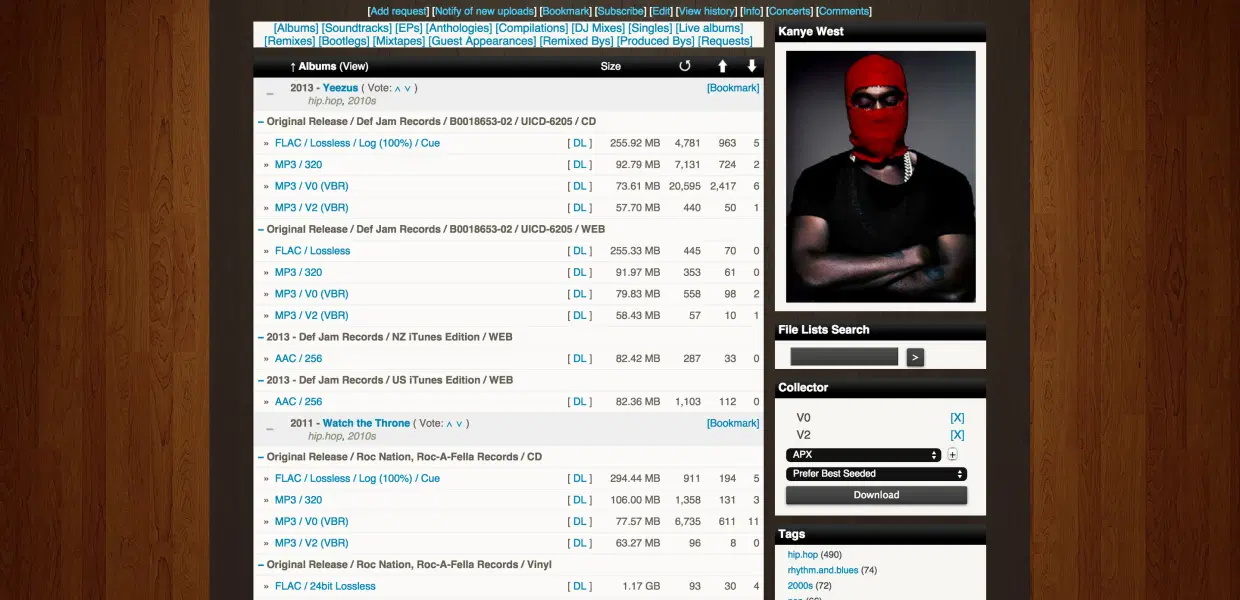
\includegraphics[width=\linewidth]{../assets/images/kanye-what.png} \emph{The
what.cd artist page for Kanye West (taken from
\href{https://qz.com/840661/what-cd-is-gone-a-eulogy-for-the-greatest-music-collection-in-the-world/}{here}
in the style of pirates, without permission). For the album ``Yeezus,''
there are ten torrents, grouped by each time the album was released on
CD and Web, and in multiple different qualities and formats (.flac,
.mp3). Along the top is a list of the macro-level groups, where what is
in view is the ``albums'' section, there are also sections for bootleg
recordings, remixes, live albums, etc.}

What.cd was a ``private'' bittorrent tracker, where unlike public
trackers that anyone can access, membership was strictly limited to
those who were personally invited or to those who passed an interview
(for more on public and private tracker, see \cite{meulpolderPublicPrivateBitTorrent} ). Invites were extremely rare,
and the interview process was demanding to the point where
\href{https://opentrackers.org/whatinterviewprep.com/index.html}{extensive
guides} were written to prepare for them.

The what.cd incentive system was based on a required ratio of data
uploaded vs.~data downloaded \cite{jiaHowSurviveThrive2013} .
Peer to peer systems need to overcome a free-rider problem where users
might download a torrent (``leeching'') and turn their computer off,
rather than leaving their connection open to share it to others (or,
``seeding''). In order to download additional music, then, one would
have to upload more. Since downloading is highly restricted, and
everyone is trying to upload as much as they can, torrents had a large
number of ``seeders,'' and even rare recordings would be sustained for
years, a pattern common to private trackers \cite{liuUnderstandingImprovingRatio2010} .

The high seeder/leecher ratio made it so it was extremely difficult to
acquire upload credit, so users were additionally incentivized to find
and upload new recordings to the system. What.cd implemented a
``bounty'' system, where users with a large amount of excess upload
credit would be able to offer some of it to whoever was able to upload
the album they wanted. To ``prime the pump'' and keep the economy
moving, highlight artists in an album of the week, or direct users to
preserve rare recordings, moderators would also use a ``freeleech''
system, where users would be able to download a specified set of
torrents without it counting against their download quantity \cite{kashEconomicsBitTorrentCommunities2012, chenImprovingSustainabilityPrivate2011a} .

The other half of what.cd was the more explicitly social elements: its
forums, comment sections, and moderation systems. The forum was home to
roiling debates that lasted years about the structure of some tagging
schema, whether one genre was just another with a different name, and so
on. The structure of the community was an object of constant, public
negotiation, and over time the metadata system evolved to be able to
support a library of the entirety of human music output\footnote{Though
  music metadata might seem like a trivial problem (just look at the
  fields in an MP3 header), the number of edge cases are profound. How
  would you categorize an early Madlib casette mixtape remastered and
  uploaded to his website where he is mumbling to himself while
  recording some live show performed by multiple artists, but on the
  b-side is one of his Beat Konducta collections that mix together
  studio recordings from a collection of other artists? Who is the
  artist? How would you even identify the unnamed artists in the live
  show? Is that a compilation or a bootleg? Is it a cassette rip, a
  remaster, or a web release?}, and the rules and incentive structures
were made to align with building it. To support the good operation of
the site, the forums were also home to a huge amount of technical
knowledge, like guides on how to make a perfect upload, that eased new
users into being able to use the system.

A critical problem in maintaining coherent databases is correcting
metadata errors and departures from schemas. Finding errors was
rewarded. Users were able to discuss and ask questions of the uploader
in a comment section below each upload, which would allow ``polite''
resolution of low-level errors like typos. More serious problems could
be reported to the moderation team, which caused the upload to be
visibly marked as under review, and the report could then be discussed
either in the comment sections or the forum. Being an anonymous,
gray-area community, there was of course plenty of power that was
tripped on. Rather than being a messy hodgepodge of fake, low-quality
uploads, though, what.cd was always teetering just shy of perfection.

These structural considerations do not capture the most elusive but
indisputably important features of what.cd's community infrastructure:
\emph{the sense of commmunity}. The What.cd forums were the center of
many user's relationships to music. Threads about all the finest scales
of music nichery could last for years: it was a rare place people who
probably cared a little bit too much about music could talk to people
with the same condition. What made it more satisfying than other music
forums was that no matter what music you were talking about, everyone
else in the conversation would always have access to it if they wanted
to hear it. Beyond any structural incentives, people spent so much time
building and maintaining what.cd because it became a source of community
and a sink of personal investment.

Structural norms supported by social systems converge as a sort of
\emph{reputational} incentive. Uploading a new album to fill a bounty
both makes the network more functional and complete, but also
\emph{people respect you for it} because it's prominently displayed on
your profile as well as in the bounty charts and that \emph{feels good}.
Becoming known on the forums for answering questions, writing guides, or
even just having a good taste in music \emph{feels good} and also
contributes to the overall health of the system. Though there are plenty
of databases, and even plenty of different communication venues for
scientists, there aren't any databases (to my knowledge) with integrated
community systems.

The tracker overlay model mirrors and extends some of the
recommendations made by Benedikt Fecher and colleagues in their work on
the reputational economy surrounding data sharing \cite{fecherReputationEconomyHow2017} . They give three policy
recommendations: Increasing reputational benefits, reducing transaction
costs, and ``increasing market transparency by making open access to
research data more visible to members of the research community.'' One
way to accomplish implement them is to embed a data sharing system
within a social system that is designed to reward communitarian
behavior.

Many features of what.cd's structure are undesirable for scientific
infrastructure, but they demonstrate that a robust archive is not only a
matter of building a database with some frontend, but by building a
community \cite{brossCommunityCollaborationContribution2013} . Of
course, we need to be careful with building the structural incentives
for a data sharing system: the very last thing we want is another
\href{https://etiennelebel.com/cs/t-leaderboard/t-leaderboard.html}{coercive
leaderboard}. In contrast to what.cd, for infrastructure we want
extremely low barriers to entry, and be agnostic to resources ---
researchers with access to huge server farms should not be unduly
favored. We should think carefully about using downloading as the
``cost,'' because downloading and analyzing huge amounts of data can be
\emph{good} and exactly what we \emph{want} in some circumstances, but a
threat to privacy and data governance in others.

This model has its own problems, including the lack of interoperability
between different trackers, the need to recreate a new set of accounts
and database for each new tracker, among others. It's also been tried
before: sharing data in specific formats (as our running example,
Neurodata Without Borders) on indexing systems like bittorrent trackers
amounts to something like BioTorrents \cite{langilleBioTorrentsFileSharing2010}  or
\href{https://academictorrents.com/}{AcademicTorrents} \cite{cohenAcademicTorrentsCommunityMaintained2014} . Even with our
extensions of version control and some model of automatic mirroring of
data across the network, we still have some work to do. To address these
and several other remaining needs for scientific data infrastructure, we
can take inspiration from \emph{federated systems.}


\end{multicols}


\hypertarget{linked-data-or-surveillance-capitalism}{%
\subsubsection{Linked Data or Surveillance
Capitalism?}\label{linked-data-or-surveillance-capitalism}}


\begin{multicols}{2}
 There is no shortage of databases for scientific data, but
their traditional structure chokes on the complexity of representing
multi-domain data. Typical relational databases require some formal
schema to structure the data they contain, which have varying
reflections in the APIs used to access them and interfaces built atop
them. This broadly polarizes database design into domain-specific and
domain-general\footnote{To continue the analogy to bittorrent trackers,
  an example domain-specific vs.~domain-general dichotomy might be
  What.cd (with its specific formatting and aggregation tools for
  representing artists, albums, collections, genres, and so on)
  vs.~ThePirateBay (with its general categories of content and otherwise
  search-based aggregation interface)}. This design pattern results in a
fragmented landscape of databases with limited interoperability. In a
moment we'll consider \emph{federated systems} as a way to resolve this
dichotomy and continue developing the design of our p2p data
infrastructure, but for now we need a better sense of the problem.

Domain-specific databases require data to be in one or a few specific
formats, and usually provide richer tools for manipulating and querying
by metadata, visualization, summarization, aggregation that are
purpose-built for that type of data. For example, NIH's
\href{https://www.ncbi.nlm.nih.gov/gene/12550}{Gene} tool has several
visualization tools and cross-referencing tools for finding expression
pathways, genetic interactions, and related sequences (Figure xx). This
pattern of database design is reflected at several different scales,
through institutional databases and tools like the Allen
\href{https://connectivity.brain-map.org/}{brain atlases} or
\href{http://observatory.brain-map.org/visualcoding/}{observatory}, to
lab- and project-specific dashboards. This type of database is natural,
expressive, and powerful --- for the researchers they are designed for.
While some of these databases allow open data submission, they often
require explicit moderation and approval to maintain the guaranteed
consistency of the database, which can hamper mass use.

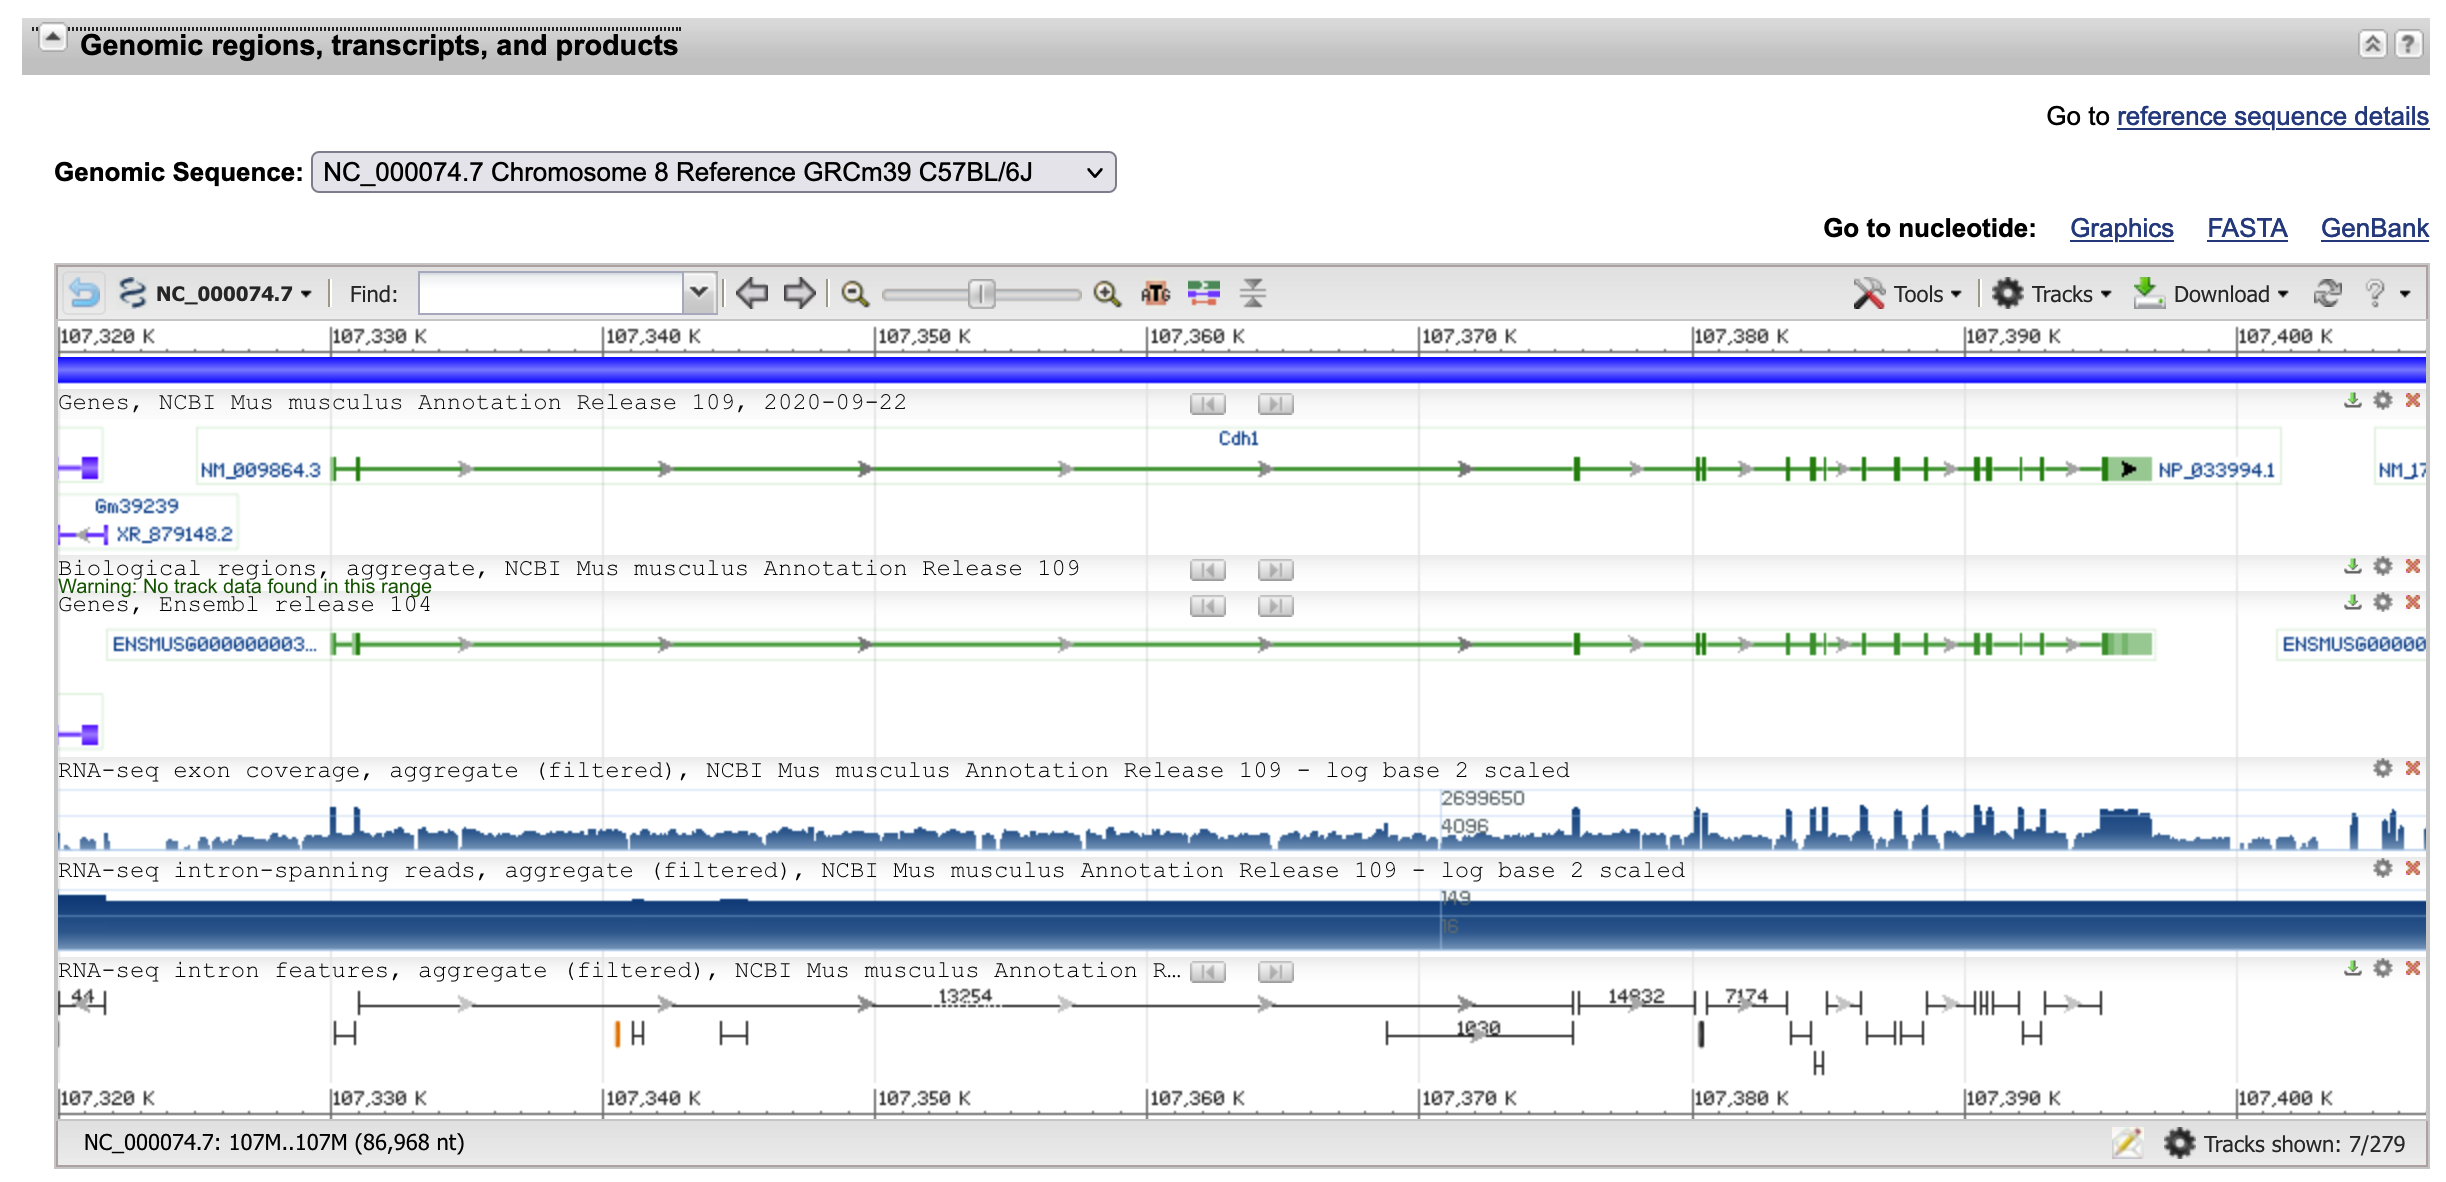
\includegraphics[width=\linewidth]{../assets/images/nih_gene_cdh1.png}
\emph{NIH's Gene tool included many specific tools for visualizing,
cross-referencing, and aggregating genetic data. Shown is the ``genomic
regions, transcripts, and product'' plot for Mouse Cdh1, which gives
useful, common summary descriptions of the gene, but is not useful for,
say, visualizing reading proficiency data.}

General-purpose databases like \href{https://figshare.com/}{figshare}
and \href{https://zenodo.org/}{zenodo}\footnote{No shade to Figshare,
  which, among others, paved the way for open data and are a massively
  useful thing to have in society.} are useful for the mass aggregation
of data, typically allowing uploads from most people with minimal
barriers. Their general function limits the metadata, visualization, and
other tools that are offered by domain-specific databases, however, and
are essentially public, versioned, folders with a DOI. Most have fields
for authorship, research groups, related publications, and a
single-dimension keyword or tags system, and so don't programmatically
reflect the metadata present in a given dataset.

The dichotomy of fragmented, subdomain-specific databases and
general-purpose databases makes combining information from across even
extremely similar subdisciplines combinatorically complex and laborious.
In the absence of a formal interoperability and indexing protocol
between databases, even \emph{finding} the correct subdomain-specific
database can be an act of raw experience or the raw luck of stumbling
across just the right blog post list of databases. It also puts
researchers who want to be good data stewards in a difficult position:
they can hunt down the appropriate subdomain specific database and risk
general obscurity; use a domain-general database and make their work
more difficult for themselves and their peers to use; or spend all the
time it takes to upload to multiple databases with potentially
conflicting demands on format.

What can be done? There are a few parsimonious answers from
standardizing different parts of the process: If we had a universal data
format, then interoperability becomes trivial. Conversely, we could make
a single ur-database that supports all possible formats and tools.

Universalizing a single part of a database system is unlikely to work
because organizing knowledge is intrinsically political. Every system of
representation is necessarily rooted in its context: one person's
metadata is another person's data. Every subdiscipline has conflicting
\emph{representational} needs, will develop different local terminology,
allocate differing granularity and develop different groupings and
hierarchies for the same phenomena. At mildest, differences in
representational systems can be incompatible, but at their worst they
can reflect and reinforce prejudices and become tools of intellectual
and social power struggles. Every subdiscipline has conflicting
\emph{practical} needs, with infinite variation in privacy demands,
different priorities between storage space, bandwidth, and computational
power, and so on. In all cases the boundaries of our myopia are
impossible to gauge: we might think we have arrived at a suitable schema
for biology, chemistry, and physics\ldots{} but what about the
historians?

Matthew J Bietz and Charlotte P Lee articulate this tension better than
I can in their ethnography of metagenomics databases:

\begin{quote}
``Participants describe the individual sequence database systems as if
they were shadows, poor representations of a widely-agreed-upon ideal.
We find, however, that by looking across the landscape of databases, a
different picture emerges. Instead, \textbf{each decision about the
implementation of a particular database system plants a stake for a
community boundary. The databases are not so much imperfect copies of an
ideal as they are arguments about what the ideal Database should be.}
{[}\ldots{]}

When the microbial ecology project adopted the database system from the
traditional genomic ``gene finders,'' they expected the database to be a
boundary object. They knew they would have to customize it to some
extent, but thought it would be able to ``travel across borders and
maintain some sort of constant identity''. In the end, however,
\textbf{the system was so tailored to a specific set of research
questions that the collection of data, the set of tools, and even the
social organization of the project had to be significantly changed.} New
analysis tools were developed and old tools were discarded. Not only was
the database ported to a different technology, the data itself was
significantly restructured to fit the new tools and approaches. While
the database development projects had begun by working together, in the
end they were unable to collaborate. \textbf{The system that was
supposed to tie these groups together could not be shielded from the
controversies that formed the boundaries between the communities of
practice.}'' \cite{bietzCollaborationMetagenomicsSequence2009} 
\end{quote}

As one ascends the scales of formalizing to the heights of the ontology
designers, the ideological nature of the project is like a klaxon
(emphasis in original):

\begin{quote}
An exception is the Open Biomedical Ontologies (OBO) Foundry initiative,
which accepts under its label only those ontologies that adhere to the
principles of ontological realism. {[}\ldots{]} Ontologies, from this
perspective, are representational artifacts, comprising a taxonomy as
their central backbone, whose representational units are intended to
designate \emph{universals} (such as \emph{human being} and
\emph{patient role}) or \emph{classes defined in terms of universals}
(such as \emph{patient,} a class encompassing \emph{human beings} in
which there inheres a \emph{patient role}) and certain relations between
them. {[}\ldots{]}

BFO is a realist ontology {[}15,16{]}. This means, most importantly,
that representations faithful to BFO can acknowledge only those entities
which exist in (for example, biological) reality; thus they must reject
all those types of putative negative entities - lacks, absences,
non-existents, possibilia, and the like \cite{ceustersFoundationsRealistOntology2010} 
\end{quote}

Aside from unilateral standardization, another formulation that doesn't
require existing server infrastructure to be dramatically changed is to
link existing databases. The problem of linking databases is an old one
with much well-trodden ground, and in the current regime of large server
farms tend to find themselves somewhere close to metadata-indexing
overlays. These overlays provide some additional tool that can translate
and combine data between databases with some mapping between the
terminology in the overlay and that of the individual databases. The NIH
articulates this as a ``Biomedical Data Translator'' in its Strategic
plan for Data Science:

\begin{quote}
Through its Biomedical Data Translator program, the National Center for
Advancing Translational Sciences (NCATS) is supporting research to
develop ways to connect conventionally separated data types to one
another to make them more useful for researchers and the public. The
Translator aims to bring data types together in ways that will integrate
multiple types of existing data sourcess, including objective signs and
symptoms of disease, drug effects, and other types of biological data
relevant to understanding the development of disease and how it
progresses in patients. \cite{NIHStrategicPlan2018} 
\end{quote}

And NCATS elaborates it a bit more on the project
\href{https://ncats.nih.gov/translator/about}{``about''} page:

\begin{quote}
As a result of recent scientific advances, a tremendous amount of data
is available from biomedical research and clinical interactions with
patients, health records, clinical trials and adverse event reports that
could be useful for understanding health and disease and for developing
and identifying treatments for diseases. Ideally, these data would be
mined collectively to provide insights into the relationship between
molecular and cellular processes (the targets of rational drug design)
and the signs and symptoms of diseases. Currently, these very rich yet
different data sources are housed in various locations, often in forms
that are not compatible or interoperable with each other. -
https://ncats.nih.gov/translator/about
\end{quote}

The Translator is being developed by 28 institutions and nearly 200 team
members as of 2019. They credit their group structure and flexible Other
Transaction Award (OTA) funding mechanism for their successes \cite{consortiumBiomedicalDataTranslator2019} . OTA awards give the
granting agency broad flexibility in to whom and for what money can be
given, and consist of an initial competetive segment with possibility
for indefinite noncompetitive extensions at the discretion of the agency
\cite{fleisherOtherTransactionAward2019} .

The project appears to be in a relatively early phase, and so it's
relatively difficult to figure out exactly what it is that has been
built. The
\href{https://web.archive.org/web/20210710012427/https://ncats.nih.gov/translator/projects}{projects
page} is currently a list of the leaders of different areas, but some
parts of the project are visible through a bit of searching. They
describe a registry of APIs for existing databases collected on their
platform \href{https://smart-api.info/portal/translator}{SmartAPI} that
are to be combined into a semantic knowledge graph \cite{consortiumUniversalBiomedicalData2019} . There are many kinds of
knowledge graphs, and we will return to them and other semantic web
technologies in \protect\hyperlink{shared-knowledge}{shared knowledge},
but the Translator's knowledge graph explicitly sits ``on top'' of the
existing databases as the only source of knowledge. Specifically, the
graph structure consists of the nodes and edges of the
\href{https://github.com/biolink/biolink-model}{biolink model} \cite{bruskiewichBiolinkBiolinkmodel2021} , and an edge is matched to a
corresponding API that provides data for both elements. For each edge in
the graph, then, a number of possible APIs can provide data without
necessarily making a guarantee of consistency or accuracy.

They articulate a very similar set of beliefs about the impossibility of
a unified dataset or ontology\footnote{\begin{quote}
  First, we assert that a single monolithic data set that directly
  connects the complete set of clinical characteristics to the complete
  set of biomolecular features, including ``-omics'' data, will never
  exist because the number of characteristics and features is constantly
  shifting and exponentially growing. Second, even if such a single
  monolithic data set existed, all-vs.-all associations will inevitably
  succumb to problems with statistical power (i.e., the curse of
  dimensionality).9 Such problems will get worse, not better, as more
  and more clinical and biomolecular data are collected and become
  available. We also assert that there is no single language, software
  or natural, with which to express clinical and biomolecular
  observations---these observations are necessarily and appropriately
  linked to the measurement technologies that produce them, as well as
  the nuances of language. The lack of a universal language for
  expressing clinical and biomolecular observations presents a risk of
  isolation or marginalization of data that are relevant for answering a
  particular inquiry, but are never accessed because of a failure in
  translation.

  Based on these observations, our final assertion is that automating
  the ability to reason across integrated data sources and providing
  users who pose inquiries with a dossier of translated answers coupled
  with full provenance and confidence in the results is critical if we
  wish to accelerate clinical and translational insights, drive new
  discoveries, facilitate serendipity, improve clinical-trial design,
  and ultimately improve clinical care. This final assertion represents
  the driving motivation for the Translator system. \cite{consortiumUniversalBiomedicalData2019} 
  \end{quote}}\cite{consortiumUniversalBiomedicalData2019} ,
although arguably create one in
\href{https://biolink.github.io/biolink-model/docs/}{biolink}, and this
problem seems to have driven the focus of the project away from linking
data as such towards developing a graph-powered query engine. The
Translator is being designed to use machine-learning powered
``autonomous relay agents'' that sift through the inhomogenous data from
the APIs and are able to return a human-readable response, also
generated with machine-learning. The final form of the translator is
still unclear, but between
\href{https://smart-api.info/portal/translator}{SmartAPI}, a
seemingly-preliminary description of the reasoning engine \cite{goelExplanationContainerCaseBased2021} , and descriptions from
contractors \cite{ROBOKOPCoVar2021} , the machine learning
component of the system could make it quite dangerous.

The intended use of the Translator seems to not be to directly search
for and use the data itself, but to use the connected data to answer
directed questions \cite{goelExplanationContainerCaseBased2021} 
--- an example that is used repeatedly is drug discovery. For any given
query of ``drugs that could treat x disease,'' the system traces out the
connected nodes in the graph from the disease to find its phenotypes,
which are connected to genes, which might be connected to some drug, and
so on. The Translator builds on top of a large number of databases and
database aggregators, and so it then needs a way of comparing and
ranking possible answers to the question. In a simple case, a drug that
directly acted on several involved genes might be ranked higher than,
say, one that acted only indirectly on phenotypes with many off-target
effects.

As with any machine-learning based system, if the input data is biased
or otherwise (inevitably) problematic then the algorithm can only
reflect that. If it is the case that this algorithm remains proprietary
(due to, for example, it being developed by a for-profit defense
contractor that named it ROBOKOP \cite{ROBOKOPCoVar2021} )
harmful input data could have unpredictable long-range consequences on
the practice of medicine as well as the course of medical research.
Taking a very narrow sample of APIs that return data about diseases, I
queried \href{https://mydisease.info}{mydisease.info} to see if it still
had the outmoded definition of ``transsexualism'' as a disease \cite{ramTransphobiaEncodedExamination2021} . Perhaps unsurprisingly, it
did, and was more than happy to give me a list of genes and variants
that supposedly ``cause'' it -
\href{http://mydisease.info/v1/query?q=\%22DOID\%3A10919\%22}{see for
yourself}.

This is, presumably, the fragility and inconsistency the
machine-learning layer was intended to putty over: if one follows the
provenance of the entry for ``gender identity disorder'' (renamed in
DSM-V), one reaches first the disease ontology
\href{https://web.archive.org/web/20211007053446/https://www.ebi.ac.uk/ols/ontologies/doid/terms?iri=http\%3A\%2F\%2Fpurl.obolibrary.org\%2Fobo\%2FDOID_1234}{DOID:1234}
which seems to trace back into an entry in a graph aggregator
\href{http://www.ontobee.org/ontology/DOID?iri=http://purl.obolibrary.org/obo/DOID_1234}{Ontobee}
(\href{https://web.archive.org/web/20210923110103/http://www.ontobee.org/ontology/DOID?iri=http://purl.obolibrary.org/obo/DOID_1234}{Archive
Link}), which in turn lists this
\href{https://github.com/jannahastings/mental-functioning-ontology}{github
repository} \textbf{maintained by a single person} as its
source\footnote{I submitted a
  \href{https://github.com/jannahastings/mental-functioning-ontology/pull/8}{pull
  request} to remove it. A teardrop in the ocean.}.

If at its core the algorithm believes that being transgender is a
disease, could it misunderstand and try to ``cure'' it? Even if it
doesn't, won't it influence the surrounding network of entities with its
links to genes, prior treatment, and so on in unpredictable ways?
Combined with the online training that is then shared by other users of
the translator \cite{consortiumUniversalBiomedicalData2019} ,
socially problematic treatment and research practices could be built
into our data infrastructure without any way of knowing their effect. In
the long-run, an effort towards transparency could have precisely the
opposite effect by being run through a series of black boxes.

A larger problem is reflected in the scope and evolving direction of the
Translator when combined with the preceding discussion of putting all
data in the hands of cloud platform holders. There is mission creep from
the original NIH initiative language that essentially amounts to a way
to connect different data sources --- what could have been as simple as
a translation table between different data standards and formats. The
original
\href{https://web.archive.org/web/20210709100523/https://ncats.nih.gov/news/releases/2016/feasibility-assessment-translator}{funding
statement from 2016} is similarly humble, and press releases
\href{https://web.archive.org/web/20210709171335/https://ncats.nih.gov/pubs/features/translator}{through
2017} also speak mostly in terms of querying the data -- though some
ambition begins to creep in.

That is remarkably different than what is articulated in 2019 \cite{consortiumUniversalBiomedicalData2019}  to be much more focused on
\emph{inference} and \emph{reasoning} from the graph structure of the
linked data for the purpose of \emph{automating drug discovery.} It
seems like the original goal of making a translator in the sense of
``translating data between formats'' has morphed into ``translating data
to language,'' with ambitions of providing a means of making algorithmic
predictions for drug discovery and clinical practice rather than linking
data \cite{hailuNIHfundedProjectAims2019}  Tools like these have
been thoroughly problematized elsewhere, eg. \cite{groteEthicsAlgorithmicDecisionmaking2020, obermeyerDissectingRacialBias2019, panchArtificialIntelligenceAlgorithmic2019, panchInconvenientTruthAI2019} .

As of September 2021, it appears there is still some work left to be
done to make the Translator functional, but the early example
illustrates some potential risks (emphases mine):

\begin{quote}
The strategy used by the Translator consortium in this case is to 1)
identify phenotypes that are associated with {[}Drug-Induced Liver
Injury{]} DILI, then 2) find genes which are correlated with these
presumably pathological phenotypes, and then 3) identify drugs which
target those genes' products. The rationale is that drugs which target
gene products associated with phenotypes of DILI may possibly serve as
candidates for treatment options.

\textbf{We constructed a series of three queries,} written in the
Translator API standard language and submitted to xARA to select
appropriate KPs to collect responses (Figure 4). \textbf{From each
response, an exemplary result is selected and used in the query for the
next step.}

The results of the first query produced several phenotypes, one of them
was ''Red blood cell count'' (EFO0004305). When using this phenotype in
the second step to query for genes, we identified one of the results as
the telomerase reverse transcriptase (TERT) gene. This was then used in
the third query (Figure 4) to identify targeting drugs, which included
the drug Zidovudine.

xARA use this result to call for an explanation. The xcase retrieved
uses a relationship extraction algorithm {[}6{]} fine-tuned using
BioBert {[}7{]}. The explanation solution seeks previously pre-processed
publications where both biomedical entities (or one of its synonyms) is
found in the same article within a distance shorter than 10 sentences.
The excerpt of entailing both terms is then used as input to the
relationship extraction method. When implementing this solution for the
gene TERT (NCBIGene:7015) and the chemical substance Zidovudine
(CHEBI:10110), the solution was able to identify corroborating evidence
of this drug-target interaction with the relationship types being one
of: ''DOWNREGULATOR,'' ''INHIBITOR,'' or ''INDIRECT DOWNREGULATOR'' with
respect to TERT. \cite{goelExplanationContainerCaseBased2021} 
\end{quote}

As a recap, since I'm not including the screenshots of the queries, the
researchers searched first for a phenotypic feature of DILI, then
selected ``one of them'' --- red blood cell count --- to search for
genes that affect the phenotype, and eventually find a drug that effects
that gene: all seemingly manually (an additional \$1.4 million has been
allocated to unify them \cite{haendelCommonDialectInfrastructure2021} ). Zidovudine, as a nucleoside reverse transcriptase inhibitor, does
inhibit telomerase reverse transcriptase \cite{hukezalieVitroExVivo2012} , but can also cause anemia and lower red
blood cell counts \cite{ZidovudinePatientNIH}  -- so through the
extended reasoning chain the system has made a sign flip and recommended
a drug that will likely make the identified phenotype (low red blood
cell count) worse? The manual input will then be used to train the
algorithm for future results, though how data from prior use and data
from graph structure will be combined in the ranking algorithm --- and
then communicated to the end user --- is still unclear.

Contrast this with the space-age and chromed-out description from CoVar:

\begin{quote}
ROBOKOP technology scours vast, diverse databases to find answers that
standard search technologies could never provide. It does much more than
simple web-scraping. It considers inter-relationships between entities,
such as colds cause coughs. Then it searches for new connections between
bits of knowledge it finds in a wide range of data sources and generates
answers in terms of these causal relationships, on-the-fly.

Instead of providing a simple list of responses, ROBOKOP ranks answers
based on various criteria, including the amount of supporting evidence
for a claim, how many published papers reference a given fact, and the
specificity of any particular relationship to the question.
\end{quote}

For-profit platform holders are not incentivized to do responsible
science, or even really make something that works, provided they can get
access to some of the government funding that pours out for projects
that are eventually canned -
\href{https://reporter.nih.gov/search/kDJ97zGUFEaIBIltUmyd_Q/projects?sort_field=FiscalYear\&sort_order=desc}{\$75.5
million} so far since 2016 for the Translator \cite{RePORTRePORTERBiomedical2021} . As exemplified by the trial and
discontinuation of the NIH Data Commons after
\href{https://reporter.nih.gov/search/H4LxgMGK9kGw6SeWCom85Q/projects?shared=true}{\$84.7
million}, centralized infrastructure projects often an opportunity to
``dance until the music stops.'' Again, it is relatively difficult to
see from the outside what work is going on and how it all fits together,
but judging from RePORTER there seem to be a
\href{https://reporter.nih.gov/project-details/10332268}{profusion} of
\href{https://reporter.nih.gov/project-details/10333468}{projects} and
\href{https://reporter.nih.gov/project-details/10333460}{components} of
the \href{https://reporter.nih.gov/project-details/10330627}{system}
with unclear functional overlap, and the model seems to have developed
into allocating funding to develop each separate knowledge source.

The risk with this project is very real because of the context of its
development. After 5 years, it still seems like the the Translator is
relatively far from realizing the vision of biopolitical control through
algorithmic predictions, but combined with Amazon's aggressive expansion
into health technology \cite{AWSAnnouncesAWS2021}  and even
literally providing \href{https://amazon.care/}{health care} \cite{lermanAmazonBuiltIts2021} , and the uploading of all scientific and
medical data onto AWS with entirely unenforceable promises of data
privacy \cite{quinnYouCanTrust2021}  --- the notion of spending
public money to develop a system for aggregating patient data with
scientific and clinical data becomes dangerous. It doesn't require
takeover by Amazon to become dangerous --- once you introduce the need
for data to train an algorithm, you need to feed it data, and so the
translator gains the incentive to suck up as much personal and other
data as it can.

!! It doesn't even need to be Amazon, the publishers are getting into it
too! RELX owns lexisnexis, a big identity management company, and is
aggressively building out its machine-learning tools for science. From
their 2019 annual shareholders report:

\begin{quote}
Elsevier serves academic and government research administrators and
leaders through its Research Intelligence suite of products. SciVal is a
decision tool that helps institutions to establish, execute and evaluate
research strategies by leveraging bibliometric data {[}\ldots{]}
Elsevier expanded its leadership position in research institution
benchmarking analytics through further investment in its SciVal Topic
Prominence in Science. Big data technology takes into consideration
nearly all of the articles available in Scopus since 1996 and clusters
them into nearly 96,000 global, unique research topics based on
citations patterns.

Elsevier's flagship clinical reference platform, ClinicalKey, provides
physicians, nurses and pharmacists with access to leading Elsevier and
third-party reference and evidence-based medical content {[}\ldots{]}
Elsevier has developed a Healthcare Knowledge Graph, which utilises ML
and Natural Language Processing (NLP) to knit together its collection of
the world's foremost clinical knowledge. The Healthcare Knowledge Graph
enhances ClincialKey, the portal into Elsevier's vast medical content
library by providing more timely clinical results for users.

{[}\ldots{]} For healthcare professionals, Elsevier's clinical solutions
include Interactive Patient Education and Care Planning. Elsevier's
ClinicalPath (formerly Via Oncology) provides clinical pathways
delivering personalised, evidence-based oncology guidance at the point
of care. Elsevier's analytics capabilities in oncology support our
ClinicalPath customers in answering increasingly complex questions
around the delivery of cancer care, such as appropriate use of precision
oncology and treatment adherence.
\end{quote}

!! So not only do we risk distorting the practice of medicine, we could
distort the entire trajectory of science. SciVal autoranks researchers
and institutions based on how ``hot'' their research programs are, and
helps suggest topics that are more likely to get a grant, etc. Since
they also aggressively control what gets recommended, and have also
recently started literally selling ads on their websites, they could
easily create the same kind of informational bubbles that we are
familiar with from social media. And with the combination of a
biomedical knowledge graph contiguous with the pharmaceutical industry,
they could steer all basic research --- perhaps with us being only dimly
aware --- to support the profit of their pharmaceutical partners. This
isn't even speculative !
https://www.elsevier.com/solutions/biology-knowledge-graph

Even assuming the Translator works perfectly and has zero unanticipated
consequences, the development strategy still reflects the inequities
that pervade science rather than challenge them. Biopharmaceutical
research, followed by broader biomedical research, being immediately and
extremely profitable, attracts an enormous quantity of resources and
develops state of the art infrastructure, while no similar
infrastructure is built for the rest of science, academia, and society.

Trans health {example of potential harms}

I have no doubt that everyone working on the Translator is doing so for
good reasons, and they have done useful work. Forming a consortium and
settling on a development model is hard work and this group should be
applauded for that. Unifying APIs with Smart-API, drafting an ontology,
and making a knowledge graph, are all directly useful to reducing
barriers to desiloing data and shared in the vision articulated here.

The problems here come in a few mutually reinforcing flavors, I'll group
them crudely into the constraints of existing infrastructure,
centralized models of development, and a misspecification of what the
purpose of the infrastructure should be.

Navigating a relationship with existing technology in new development is
tricky, but there is a distinction between integrating with it and
embodying its implications. Since the other projects spawned from the
Data Science Initiative embraced the use of cloud storage, the
constraint of using centralized servers with the need for a linking
overlay was baked in the project from the beginning. From this decision
immediately comes the impossibility of enforcing privacy guarantees and
the rigidity of database formats and tooling. Since the project started
from a place of presuming that the data would be hosted ``out there''
where much of its existence is prespecified, building the Translator
``on top'' of that system is a natural conclusion. Further, since the
centralized systems proposed in the other projects don't aim to provide
a means of standardization or integration of scientific data that
doesn't already have a form, the reliance on APIs for access to
structured data follows as well.

Organizing the process as building a set of tools as a relatively large,
but nonetheless centralized and demarcated group pose additional
challenges. I won't speculate on the incentives and personal dynamics
that led there, but I also believe this development model comes from
good intention. While there is clearly a lot of delegation and
distributed work, the project in its different teams takes on specific
tools that \emph{they} build and \emph{we} use. This is broadly true of
scientific tools, especially databases, and contributes to how they
\emph{feel}: they feel disconnected with our work, don't necessarily
help us do it more easily or more effectively, and contributing to them
is a burdensome act of charity.

This is reflected in the form of the biolink ontology, where rather than
a tool for scientists to \emph{build} ontologies, it is intended to be
\emph{built towards.} There is tension between the articulated
impossibility of a grand unified ontology and the eventual form of the
algorithm that depends on one that, in their words, motivated the turn
to machine learning to reconcile that impossibility. The compromise
seems to be the use of a quasi-``neutral'' meta-ontology that
instantiates its different abstract objects depending on the contents of
its APIs. A ranking algorithm to parse the potentially infinite results
follows, and so too does the need for feedback and training and the
potential for long-lived and uninterrogatable algorithmic bias.

These all contribute to the misdirection in the goal of the project.
Linking \emph{all} or \emph{most} biomedical data in single mutually
coherent system drifted into an API-driven knowledge-graph for
pharmaceutical and clinical recommendations. Here we meet a bit of a
reprise of the \protect\hyperlink{neatness-vs-scruffiness}{\#neat}
mindset, which emphasizes global coherence as a basis for reasoning
rather than providing a means of expressing the natural connections
between things in their local usage. Put another way, the emphasis is on
making something logically complete for some dream of
algorithmically-perfect future rather than to be useful to do the things
researchers at large want to do but find difficult. The press releases
and papers of the Translator project echo a lot of the heady days of the
semantic web\footnote{not to mention a sort of enlightenment-era
  diderot-like quest for the encyclopedia of everything} and its attempt
to link everything --- and seems ready to follow the same path of the
fledgling technologies being gobbled up by technology giants to finish
and privatize.

I think the problem with the initial and eventual goals of the
translater can be illustrated by problematizing the central focus on
linking ``all data,'' or at least ``all biomedical data.'' Who is a
system of ``all (biomedical) data'' for? Outside of metascientists and
pharmaceutical companies, I think most people are interested primarily
in the data of their colleagues and surrounding disciplines. Every
infrastructural model is an act of balancing constraints, and
prioritizing ``all data'' seems to imply ``for some people.'' Who is
supposed to be able to upload data? change the ontology? inspect the
machine learning model? Who is in charge of what? Who is a
knowledge-graph query engine useful for?

Another prioritization might be building systems for \emph{all people}
that can \emph{embed with existing practices} and \emph{help them do
their work} which typically involves accessing \emph{some data.} The
system needs to not only be designed to allow anyone to integrate their
data into it, but also to be integrated into how researchers collect and
use their data. It needs to give them firm, verifiable, and fine-grained
control over who has access to their data and for what purpose. It needs
to be \emph{multiple,} governable and malleable in local communities of
practice. Through the normal act of making my data available to my
colleague and vice versa, build on a cumulative and negotiable
understanding of the relationship between our work and its meaning.

Without too much more prefacing, let's return to the scheduled
programming. 
\end{multicols}


\hypertarget{federated-systems-of-language}{%
\subsubsection{Federated Systems (of
Language)}\label{federated-systems-of-language}}


\begin{multicols}{2}
 When last we left it, our peer-to-peer system needed some
way of linking data together. Instead of a big bucket of files as is
traditional in torrents and domain-general databases, we need some way
of exposing the metadata of disparate data formats so that we can query
for and find the particular range of datasets appropriate to our
question. !! For this section, I want to develop a notion of data
linking that's a lot closer to natural language than an engineering
specification.

Each format has a different metadata structure with different names, and
even within a single format we want to support researchers who extend
and modify the core format. Additionally, each format has a different
implementation, eg. as an hdf5 file, binary files in structured
subdirectories, SQL-like databases.

That's a lot of heterogeneity to manage, but fret not: there is hope.
Researchers navigate this variability manually as a standard part of the
job, and we can make that work cumulative by building tools that allow
researchers to communally describe and negotiate over the structure of
their data and the local relationships to other data structures. We can
extend our peer-to-peer system to be a \emph{federated database} system.

Federated systems consist of \emph{distributed}, \emph{heterogeneous},
and \emph{autonomous} agents that implement some minimal agreed-upon
standards for mutual communication and (co-)operation. Federated
databases\footnote{though there are subtleties to the terminology, with
  related terms like ``multidatabase,'' ``data integration,'' and ``data
  lake'' composing subtle shades of a shared idea. I will use federated
  databases as a single term that encompasses these multiple ideas here,
  for the sake of constraining the scope of the paper.} were proposed in
the early 1980's \cite{heimbignerFederatedArchitectureInformation1985}  and have been
developed and refined in the decades since as an alternative to either
centralization or non-integration \cite{litwinInteroperabilityMultipleAutonomous1990, kashyapSemanticSchematicSimilarities1996, hullManagingSemanticHeterogeneity1997} . Their application to the
dispersion of scientific data in local filesystems is not new \cite{busseFederatedInformationSystems1999, djokic-petrovicPIBASFedSPARQLWebbased2017, hasnainBioFedFederatedQuery2017} , but their implementation is more
challenging than imposing order with a centralized database or punting
the question into the unknowable maw of machine learning.

!! There is a lot of subtlety to the terminology surrounding
``federated'' and the typology of distributed systems generally, I am
using it more in the federated messaging sense of forming groups of
people, rather than the strict term federated databases which do imply a
standardized schema across a federation. I am largely in line with the
notion of distributed databases here \cite{hankeDefenseDecentralizedResearch2021} .

Amit Sheth and James Larson, in their reference description of federated
database systems, describe \textbf{design autonomy} as one critical
dimension that characterizes them:

\begin{quote}
Design autonomy refers to the ability of a component DBS to choose its
own design with respect to any matter, including

\begin{enumerate}
\def\labelenumi{(\alph{enumi})}
\item
  The \textbf{data} being managed (i.e., the Universe of Discourse),
\item
  The \textbf{representation} (data model, query language) and the
  \textbf{naming} of the data elements,
\item
  The conceptualization or \textbf{semantic interpretation} of the data
  (which greatly contributes to the problem of semantic heterogeneity),
\item
  \textbf{Constraints} (e.g., semantic integrity constraints and the
  serializability criteria) used to manage the data,
\item
  The \textbf{functionality} of the system (i.e., the operations
  supported by system),
\item
  The \textbf{association and sharing with other systems}, and
\item
  The \textbf{implementation} (e.g., record and file structures,
  concurrency control algorithms).
\end{enumerate}
\end{quote}

Susanne Busse and colleagues add an additional dimension of
\textbf{evolvability,} or the ability of a particular system to adapt to
inevitable changing uses and requirements \cite{busseFederatedInformationSystems1999} .

In order to support such radical autonomy and evolvability, federated
systems need some means of translating queries and representations
between heterogeneous components. The typical conceptualization of
federated databases have five layers that implement different parts of
this reconciliation process \cite{shethFederatedDatabaseSystems1990} :

\begin{itemize}

\item
  A \textbf{local schema} is the representation of the data on local
  servers, including the means by which they are implemented in binary
  on the disk
\item
  A \textbf{component schema} serves to translate the local schema to a
  format that is compatible with the larger, federated schema
\item
  An \textbf{export schema} defines permissions, and what parts of the
  local database are made available to the federation of other servers
\item
  The \textbf{federated schema} is the collection of export schemas,
  allowing a query to be broken apart and addressed to different export
  schemas. There can be multiple federated schemas to accomodate
  different combinations of export schemas.
\item
  An \textbf{export schema} can further be used to make the federated
  schema better available to external users, but in this case since
  there is no notion of ``external'' it is less relevant.
\end{itemize}

This conceptualization provides a good starting framework and isolation
of the different components of a database system, but a peer-to-peer
database system has different constraints and opportunities \cite{bonifatiDistributedDatabasesPeertopeer2008} . In the strictest,
``tightly coupled'' federated systems, all heterogeneity in individual
components has to be mapped to a single, unified federation-level
schema. Loose federations don't assume a unified schema, but settle for
a uniform query language, and allow multiple translations and views on
data to coexist. A p2p system naturally lends itself to a looser
federation, and also gives us some additional opportunities to give
peers agency over schemas while also preserving some coherence across
the system. I will likely make some database engineers cringe, but the
emphasis for us will be more on building a system to support distributed
social control over the database, rather than guaranteeing consistency
and transparency between the different components.

Though there are hundreds of subtleties and choices in implementation
beneath the level of detail I'll reach here, allow me to illustrate the
system by example:

Let us start with the ability for a peer to choose who they are
associated with at multiple scales of organization: a peer can directly
connect with another peer, but peers can also federate into groups,
groups can federate into groups of groups, and so on. Within each of
these grouping structures, the peer is given control over what data of
theirs is shared.

Clearly, we need some form of \emph{identity} in the system, let's make
it simple and flat and denote that in pseudocode as \texttt{@username}
--- in reality, without any form of distributed uniqueness checking, we
would need to have some notion of where this username is ``from,'' so
let's say we actually have a system like \texttt{username@name-provider}
but for this example assume a single name provider, say
ORCID\footnote{!! now would be the time blockchain ppl are like ``but
  wait! that's centralization! how can you trust ORCID??'' Those kinds
  of systems are designed for zero-trust environments, but we don't need
  absolute zero trust in this system since we are assuming we're
  operating with visible entities in a system already bound to some
  degree by reputation.}. Someone would then be able to use their
\texttt{@name}space as a root, under which they could refer to their
data, schemas, and so on, which will be denoted \texttt{@name:subobject}
(see this notion of personal namespaces for knowledge organization
discussed in early wiki culture here \cite{MeatballWikiPersonalCategories} ). Let us also assume that there is
no categorical difference between \texttt{@usernames} used by individual
researchers, institutions, consortia, etc. --- everyone is on the same
level.

We pick up where we left off earlier with a peer who has their data in
some discipline-specific format, which let us assume for the sake of
concreteness has a representation as an
\href{https://www.w3.org/OWL/}{OWL} schema.

That schema could be ``owned'' by the \texttt{@username} corresponding
to the standard-writing group --- eg \texttt{@nwb} for neurodata without
borders. In a \href{https://www.w3.org/TR/turtle/}{turtle-ish}
pseudocode, then, our dataset might look like this:

\begin{verbatim}
<#cool-dataset>
    a @nwb:NWBFile
    @nwb:general:experimenter @jonny
    @nwb:ElectricalSeries
        .electrodes [1, 2, 3]
        .rate 30000
        .data [...]
\end{verbatim}

Where I indicate that me, \texttt{@jonny} collected
\texttt{a\ @nwb:NWBFile} dataset (indicated with
\texttt{\textless{}\#dataset-name\textgreater{}} to differentiate an
application/instantiation of a schema from its definition) that
consisted of an \texttt{@nwb:ElectricalSeries} and the relevant
attributes (where a leading \texttt{.} is a shorthand for the parent
schema element).

!! pause to describe notion of using triplet links and the generality
they afford us.

I have some custom field for my data, though, which I extend the format
specification to represent. Say I have invented some new kind of
solar-powered electrophysiological device and want to annotate its specs
alongside my data.

\begin{verbatim}
@jonny:SolarEphys < @nwb:NWBContainer
    ManufactureDate
    InputWattageSeries < @nwb:ElectricalSeries
        newprop
        -removedprop
\end{verbatim}

!! think of a better example lmao\^{}\^{} and then annotate what's going
on.

There are many strategies for making my ontology extension available to
others in a federated network. We could use a distributed hash table, or
\href{https://en.wikipedia.org/wiki/Distributed_hash_table}{\textbf{DHT}},
like bittorrent, which distributes references to information across a
network of peers (eg. \cite{pirroDHTbasedSemanticOverlay2012} ).
We could use a strategy like the
\href{https://matrix.org/}{\textbf{Matrix} messaging protocol}, where
users belong to a single home server that federates with other servers.
Each server is responsible for keeping a synchronized copy of the
messages sent on the servers and rooms it's federated with, and each
server is capable of continuing communication if any of the others
failed. We could use
\href{https://www.w3.org/TR/2018/REC-activitypub-20180123/}{\textbf{ActivityPub}
(AP)} \cite{Webber:18:A} , a publisher-subscriber model where
users affiliated with a server post messages to their `outbox' and are
sent to listening servers (or made available to HTTP GET requests). AP
uses \href{https://json-ld.org/}{JSON-LD} \cite{spornyJSONLDJSONbasedSerialization2020} , so is already capable of
representing linked data, and the related ActivityStreams vocabulary
\cite{snellActivityStreams2017}  also has plenty of relevant
\href{https://www.w3.org/TR/activitystreams-vocabulary/\#activity-types}{action
types} for
\href{https://www.w3.org/TR/activitystreams-vocabulary/\#dfn-create}{creating},
\href{https://www.w3.org/TR/activitystreams-vocabulary/\#dfn-question}{discussing},
and
\href{https://www.w3.org/TR/activitystreams-vocabulary/\#dfn-tentativeaccept}{negotiating}
over links (also see
\href{https://github.com/openEngiadina/cpub}{cpub}). We'll return to
ActivityPub later, but for now the point is to let us assume we have a
system for distributing schemas/extensions/links associated with an
identity publicly or to a select group of peers.

For the moment our universe is limited only to other researchers using
NWB. Conveniently, the folks at NWB have set up a federating group so
that everyone who uses it can share their format extensions. Since our
linking system for manipulating schemas is relatively general, we can
use it to ``formalize'' a basic configuration for a federating group
that automatically \texttt{Accept}s request to \texttt{Join} and allows
any schema that inherits from their base \texttt{@nwb:NWBContainer}
schema. Let's say \texttt{@fed} defines some basic properties of our
federating system --- it constitutes our federating ``protocol'' --- and
loosely use some terms from the
\href{https://www.w3.org/ns/activitystreams\#class-definitions}{ActivityStreams}
vocabulary as \texttt{@as}

\begin{verbatim}
<#nwbFederation>
  a @fed:Federation
  onReceive
    @as:Join @as:Accept
  allowSchema
    extensionOf @nwb:NWBContainer
\end{verbatim}

Now anyone that is a part of the \texttt{@nwbFederation} would be able
to see the schemas we have submitted, sort of like a beefed up,
semantically-aware version of the existing
\href{https://nwb-extensions.github.io/}{neurodata extensions catalog}.
In this system, many overlapping schemas could exist simultaneously, but
wouldn't become a hopeless clutter because similar schemas could be
compared and reconciled based on their semantic properties.

So far we have been in the realm of metadata, but how would my computer
know how to read and write the data to my disk so i can use it? In a
system with heterogeneous data types and database implementations, we
need some means of specifying different programs to use to read and
write, different APIs, etc. Why not make that part of the file schema as
well? Suppose the HDF5 group (or anyone, really!) has a namespace
\texttt{@hdf} that defines the properties of an \texttt{@hdf:HDF5} file,
basic operations like \texttt{Read}, \texttt{Write}, or \texttt{Select}.
NWB could specify that in their definition of \texttt{@nwb:NWBFile}:

\begin{verbatim}
@nwb.NWBFile
  a @hdf:HDF5
    isVersion x.y.z
    hasDependency libhdf5==x.y.z
  usesContainer @nwb:NWBContainer
\end{verbatim}

The abstraction around the file implementation makes it easier for
others to consume my data, but it also makes it easier for \emph{me} to
use and contribute to the system. Making an extension to the schema
wasn't some act of charity, it was the most direct way for me to use the
tool to do what I wanted. Win-win: I get to use my fancy new instrument
and store its data by extending some existing format standard, and in
the process make the standard more complete and useful. We are able to
make my work useful by \emph{aligning the modalities of use and
contribution.}

Now that I've got my schema extension written and submitted to the
federation, time to submit my data! Since it's a p2p system, I don't
need to manually upload it, but I do want to control who gets it. By
default, I have all my NWB datasets set to be available to the
\texttt{@nwbFederation} , and I list all my metadata on, say the Society
for Neuroscience's \texttt{@sfnFederation}.

\begin{verbatim}
<#globalPermissions>
  a @fed:Permissions
  permissionsFor @jonny

  federatedWith 
    name @nwbFederation
    @fed:shareData 
      is @nwb:NWBFile

  federatedWith
    name @sfnFederation
    @fed:shareMetadata
\end{verbatim}

Let's say this dataset in particular is a bit sensitive --- say we apply
a set of permission controls to be compliant with \texttt{@hhs.HIPAA}
--- but we do want to make use of some public server space run by our
Institution, so we let it serve an encrypted copy that those I've shared
it with can decrypt. Since we've applied the \texttt{@hhs.HIPAA}
ruleset, we would be able to automatically detect if we have any
conflicting permissions, but we're doing fine in this example.

\begin{verbatim}
<#datasetPermissions>
  a @fed:Permissions
  permissionsFor @jonny:cool-dataset

  accessRuleset @hhs:HIPAA
    .authorizedRecipient <#hash-of-patient-ids>
  
  federatedWith
    name @institutionalCloud
    @fed:shareEncrypted
\end{verbatim}

Now I want to make use of some of my colleagues data. Say I am doing an
experiment with a transgenic dragonfly and collaborating with a chemist
down the hall. This transgene, known colloquially in our discipline as
\texttt{"@neuro:superstar6"} (oh-so-uncreatively ripped off by the
chemists as \texttt{"@chem:SUPER6"}) fluoresces when the dragonfly is
feeling bashful, and we have plenty of photometry data stored as
\texttt{@nwb:Fluorescence} objects. We think that its fluorescence is
caused by the temperature-dependent conformational change from blushing.
They've gathered NMR and Emission spectroscopy data in their
chemistry-specific format, say \texttt{@acs:NMR} and
\texttt{@acs:Spectroscopy}.

We get tired of having our data separated and needing to maintain a
bunch of pesky scripts and folders, so we decide to make a bridge
between our datasets. We need to indicate that our different names for
the gene are actually the same thing and relate the spectroscopy data.

Let's make the link explicit, say we use
\href{https://www.w3.org/2009/08/skos-reference/skos.html}{\texttt{@skos}}?

\begin{verbatim}
<#super-link-6>
  a @fed:Link
  
  from @neuro:superstar6
  to @chem:SUPER6
  link @skos:exactMatch
\end{verbatim}

Our \texttt{@nwb:Fluorescence} data has the emission wavelength in its
\texttt{@nwb:Fluorescence:excitation\_lambda} property\footnote{not
  really where it would be in the standard, but go with it plz}, which
is the value of their \texttt{@acs:Spectroscopy} data at a particular
value of its \texttt{wavelength}. Unfortunately, \texttt{wavelength}
isn't metadata for our friend, but a column in the
\texttt{@acs:Spectroscopy:readings} table, so for now the best we can do
is indicate that \texttt{excitation\_lambda} is one of the values in
\texttt{wavelength} and pick it up in our analysis tools.

\begin{verbatim}
<#imaging>
 a @fed:Link
 
 from @nwb:Fluorescence:excitation_lambda
 to @acs:Spectroscopy:readings
 link @fed:Subset
   valueIn "wavelength"
\end{verbatim}

This makes it much easier for us to index our data against each other
and solves a few real practical problems we were facing in our
collaboration. We don't need to do as much cleaning when it's time to
publish the data since it can be released as a single linked entity.

Rinse and repeat our sharing and federating process from our previous
schema extension, add a little bit of extra federation with the
\texttt{@acs} namespace, and in the normal course of our doing our
research we've contributed to the graph structure linking two common
data formats. Ours is one of many, with ugly little names like
\texttt{@jonny:super-link-6}\footnote{we'll return to credit assignment,
  don't worry! I wouldn't leave a friend out to dry.}. We might not have
followed the exact rules, and we only made a few links rather than a
single authoratative mapping, but if someone is interested in compiling
one down the line they'll start off a hell of a lot further than if we
hadn't contributed it!

With a protocol for how queries can be forwarded and transformed between
users and federations, one could access the same kind of complex query
structure as traditional databases with
\href{https://www.w3.org/TR/sparql11-federated-query/}{SPARQL} \cite{SPARQLFederatedQuery2013}  as has been proposed for biology many
times before \cite{simaEnablingSemanticQueries2019, djokic-petrovicPIBASFedSPARQLWebbased2017, hasnainBioFedFederatedQuery2017} . Some division in the way that data
and metadata are handled is necessary for the network to work in
practice, since we can't expect a search to require terabytes of data
transfer. A natural solution to this is to have metadata query results
point to
\href{https://en.wikipedia.org/wiki/Content-addressable_storage}{content
addressed} identifiers that are served peer to peer. A
mutable/changeable/human-readable name and metadata system that points
to a system of permanent, unique identifiers has been one need that has
hobbled IPFS, and is the direction pointed to by DataLad \cite{hankeDefenseDecentralizedResearch2021} . A
\href{https://mastodon.social/@humanetech/107155144840782386}{parallel}
\href{https://web.archive.org/web/20211024082055/https://socialhub.activitypub.rocks/t/which-links-between-activitypub-and-solid-project/529}{set}
of
\href{https://web.archive.org/web/20211024080845/https://socialhub.activitypub.rocks/t/how-solid-and-activitypub-complement-each-other-best/727}{conversations}
has been
\href{https://web.archive.org/web/20211024081238/https://forum.solidproject.org/t/discussion-solid-vs-activitypub/2685}{happening}
in the broader linked data community with regard to using ActivityPub as
a way to index data on Solid.

In this example I have been implicitly treating the
\texttt{@nwbFederation} users like bittorrent trackers, keeping track of
different datasets in their federation, but there is no reason why
queries couldn't themselves be distributed across the participating
peers, though I believe tracker-like federations are useful and might
emerge naturally. A system like this doesn't need the radical zero trust
design of, for example, some distributed ledgers, and an overlapping
array of institutional, disciplinary, interest, and so on federations
would be a good means of realizing the evolvable community structure
needed for sustained archives.

Extend this practice across the many overlapping gradients of
cooperation and collaboration in science, and on a larger scale a system
like this could serve as a way to concretize and elevate the organic,
continual negotiation over meaning and practice that centralized
ontologies can only capture as a snapshot. It doesn't have the same
guarantees of consistency or support for algorithmic reasoning as a
top-down system would in theory, but it would give us agency over the
structure of our information and have the potential to be useful for a
far broader base of researchers.

I have no idea where the physicists' store their data or what format
it's in, \emph{but the chemists might,} and the best way to get there
from here might be a dense, multiplicative web of actual practical
knowledge instead of some sparsely used corporate API.

I have been purposefully nonprescriptive about implementation and fine
details here, what have we described so far? !! short summary of
preceding section !! recall that what i am describing is protocol-like,
so having multiple implementations that evolve is sorta the point.

Like the preceding description of the basic peer-to-peer system, this
joint metadata/p2p system could be fully compatible with existing
systems. Translating between a metadata query and a means of accessing
it on heterogeneous databases is a requisite part of the system, so, for
example, there's no reason that an HTTP-based API like SmartAPI couldn't
be queried.

\href{https://www.datalad.org/}{DataLad} \cite{halchenkoDataLadDistributedSystem2021, hankeDefenseDecentralizedResearch2021}  and its application in
Neuroscience as \href{https://dandiarchive.org}{DANDI} are two projects
that are \emph{very close} to what I have been describing here ---
developing a p2p backend for datalad and derivation into a protocol
might even be a promising development path towards it.

!! close this section by taking a larger view - \cite{langilleBioTorrentsFileSharing2010}  DANDI is in on the p2p system,
as is kachery-p2p!! p2p systems already plenty in use, academic
torrents, biotorrents, libgen on IPFS !! the proof of their utility is
in the pudding, arguably when i've been talkiung about `centralized
servers' what i'm actually talking about content delivery networks,
which are effectively p2p systems -- they just own all the peers.

!! note that this is all fully compatible with existing systems and is a
superset of centralized servers with centralized schemas! 
\end{multicols}


\hypertarget{shared-tools}{%
\subsection{Shared Tools}\label{shared-tools}}


\begin{multicols}{2}
 Straddling our system for sharing data are the tools to
gather and analyze it. Experimental and analytical tools are the natural
point of extension for collectively developed scientific digital
infrastructure, and considering them together shows the combinatoric
power of integrating interoperable domains of scientific practice. In
particular, in addition to benefits from their development in isolation,
we can ask how a more broadly integrated system helps problems like
adoption and incentives for distributed work, enables a kind of deep
provenance from experiment to results, and lets us reimagine the form of
the community and communication tools for science.

This section will be relatively short compared to
\protect\hyperlink{shared-data}{shared data}. We have already
introduced, motivated, and exemplified many of the design practices of
the broader infrastructural system. There is much less to argue against
or ``undo'' in the spaces of analytical and experimental tools because
so much more work has been done, and so much more power has been accrued
in the domain of data systems. Distributed computing does have a dense
history, with huge numbers of people working on the problem, but its
hegemonic form is much closer to the system articulated below than
centralized servers are to federated semantic p2p systems. I also have
written extensively about
\protect\hyperlink{experimental-frameworks}{experimental frameworks}
before \cite{saundersAutopilotAutomatingBehavioral2019} , and
develop \href{https://docs.auto-pi-lot.com/en/latest/}{one of them} so I
will be brief at risk of repeating myself or appearing self-serving.

!! both these sections are also relatively unstandardized, so before
jumping to some protocol just yet, we can build frameworks that start
congealing the pieces en route to one.

Integrated scientific workflows have been written about many times
before, typically in the context of the ``open science'' movement. One
of the founders of the Center for Open Science, Jeffrey Spies, described
a similar ethic of toolbuilding as I have in a 2017 presentation:

\begin{quote}
Open Workflow: 1. Meet users where they are 2. Respect current
incentives 3. Respect current workflow

We could\ldots{} demonstrate that it makes research more efficient, of
higher quality, and more accessible.

Better, we could\ldots{} demonstrate that researchers will get published
more often.

Even better, we could\ldots{} make it easy

Best, we could\ldots{} make it automatic \cite{spiesWorkflowCentricApproachIncreasing2017} 
\end{quote}

To build an infrastructural system that enables ``open'' practices,
\emph{convincing} or \emph{mandating} a change are much less likely to
be successful and sustainable than focusing on building them to make
doing work easier and openness automatic. To make this possible, we
should focus on developing \emph{frameworks to build} experimental and
analysis tools, rather than developing more tools themselves.

\hypertarget{analytical-frameworks}{%
\subsubsection{Analytical Frameworks}\label{analytical-frameworks}}

The first natural companion of shared data infrastructure is a shared
analytical framework. A major driver for the need for everyone to write
their own analysis code largely from scratch is that it needs to account
for the idiosyncratic structure of everyone's data. Most scientists are
(blessedly) not trained programmers, so code for loading and negotiating
loading data is often intertwined with the code used to analyze and plot
it. As a result it is often difficult to repurpose code for other
contexts, so the same analysis function is rewritten in each lab's local
analysis repository. Since sharing raw data and code is still a
(difficult) novelty, on a broad scale this makes results in scientific
literature as reliable as we imagine all the private or semi-private
analysis code to be.

Analytical tools (anecdotally) make up the bulk of open source
scientific software, and range from foundational and general-purpose
tools like numpy \cite{harrisArrayProgrammingNumPy2020}  and
scipy \cite{virtanenSciPyFundamentalAlgorithms2020} , through
tools that implement a class of analysis like DeepLabCut \cite{mathisDeepLabCutMarkerlessPose2018a}  and scikit-learn \cite{pedregosaScikitlearnMachineLearning2011} , to tools for a specific
technique like MoSeq \cite{wiltschkoRevealingStructurePharmacobehavioral2020}  and DeepSqueak
\cite{coffeyDeepSqueakDeepLearningbased2019} . The pattern of
their use is then to build them into a custom analysis system that can
then in turn range in sophistication from a handful of
flash-drive-versioned scripts to automated pipelines.

Having tools like these of course puts researchers miles ahead of where
they would be without them, and the developers of the mentioned tools
have put in a tremendous amount of work to build sensible interfaces and
make them easier to use. No matter how much good work might be done,
inevitable differences between APIs is a relatively sizable technical
challenge for researchers --- a problem compounded by the incentives for
fragmentation described previously. For toolbuilders, many parts of any
given tool from architecture to interface have to be redesigned with
varying degrees of success each time. For science at large, with few
exceptions of well-annotated and packaged code, most results are only
replicable with great effort.

To be clear, we have reached levels of ``not the developer's fault'' to
the tune of ``API discontinuity'' being \emph{``the norm for 99\% of
software.''} Negotiating boundaries between (and even within) software
and information structures is an elemental part of computing. The only
time it becomes a conceivable problem to ``solve'' is when the problem
domain coalesces to the point where it is possible to articulate its
abstract structure as a protocol, and the incentives are great enough to
adopt it. Thankfully that's what we're trying to do here.

It's unlikely that we will solve the problem of data analysis being
complicated, time consuming, and error prone by teaching every scientist
to be a good programmer, but we can build experimental frameworks that
make analysis tools easier to build and use.

Specifically, a shared analytical framework should be

\begin{itemize}

\item
  \textbf{Modular} - Rather than implementing an entire analysis
  pipeline as a monolith, the system should be broken into minimal,
  composable modules. The threshold of what constitutes ``minimal'' is
  of course to some degree a matter of taste, but the framework doesn't
  need to make normative decisions like that. The system should support
  modularity by providing a clear set of hooks that tools can provide:
  eg. a clear place for a given tool to accept some input, parameters,
  and so on. Since data analysis can often be broken up into a series of
  relatively independent stages, a straightforward (and common) system
  for modularity is to build hooks to make a directed acyclic graph
  (DAG) of data transformation operations. This structure naturally
  lends itself to many common problems: caching intermediate results,
  splitting and joining multiple inputs and outputs, distributing
  computation over many machines, among others. Modularity is also
  needed within the different parts of the system itself -- eg. running
  an analysis chain shouldn't require a GUI, but one should be
  available, etc.
\item
  \textbf{Pluggable} - The framework needs to provide a clear way of
  incorporating external analysis packages, handling their dependencies,
  and exposing their parameters to the user. Development should ideally
  not be limited to a single body of code with a single mode of
  governance, but should instead be relatively conservative about
  requirements for integrating code, and liberal with the types of
  functionality that can be modified with a plugin. Supporting plugins
  means supporting people developing tools for the framework, so it
  needs to make some part of the toolbuilding process easier or
  otherwise empower them relative to an independent package. This
  includes building a visible and expressive system for submitting and
  indexing plugins so they can be discovered and credit can be given to
  the developers. Reciprocal to supporting plugins is being
  interoperable with existing and future systems, which the reader may
  have assumed was a given by now.
\item
  \textbf{Deployable} - For wide use, the framework needs to be easy to
  install and deploy locally and on computing clusters. A primary
  obstacle is dependency management, or making sure that the computer
  has everything needed to run the program. Some care needs to be taken
  here, as there are multiple emphases in deployability that can be in
  conflict. Deployable for who? A system that can be relatively
  challenging to use for routine exploratory data analysis but can
  distribute analysis across 10,000 GPUs has a very circumscribed set of
  people it is useful for. This is a matter of balancing design
  constraints, but we should prioritize broad access, minimal
  assumptions of technological access, and ease of use over being able
  to perform the most computationally demanding analyses possible when
  in conflict. Containerization is a common, and the most likely
  strategy here, but the interface to containers may need a lot of care
  to make accessible compared to opening a fresh .py file.
\item
  \textbf{Reproducible} - The framework should separate the
  \emph{parameterization} of a pipeline, the specific options set by the
  user, and its \emph{implementation}, the code that constitutes it. The
  parameterization of a pipeline or analysis DAG should be portable such
  that it, for example, can be published in the supplementary materials
  of a paper and reproduced exactly by anyone using the system. The
  isolation of parameters from implementation is complementary to the
  separation of metadata from data and if implemented with semantic
  triplets would facilitate a continuous interface from our data to
  analysis system. This will be explored further below and in
  \protect\hyperlink{shared-knowledge}{shared knowledge}
\end{itemize}

Thankfully a number of existing projects that are very similar to this
description are actively being built. One example is
\href{https://datajoint.io/}{DataJoint} \cite{yatsenkoDataJointSimplerRelational2018} , which recently expanded its
facility for modularity with its recent
\href{https://github.com/datajoint/datajoint-elements}{Elements} project
\cite{yatsenkoDataJointElementsData2021} . Datajoint is a system
for creating analysis pipelines built from a graph of processing stages
(among
\href{https://docs.datajoint.org/python/v0.13/intro/01-Data-Pipelines.html\#what-is-datajoint}{other
features}). It is designed around a refinement on traditional relational
data models, which is reflected throughout the system as most operations
being expressed in its particular schema, data manipulation, and query
languages. This is useful for operations that are expressed in the
system, but makes it harder to integrate external tools with their
dependencies ---
\href{https://github.com/datajoint/element-array-ephys/blob/1fdbcf12d1a518e686b6b79e9fbe77b736cb606a/Background.md}{at
the moment} it appears that spike sorting (with
\href{https://github.com/MouseLand/Kilosort}{Kilosort} \cite{pachitariuKilosortRealtimeSpikesorting2016} ) has to happen outside
of the extracellular electrophysiology elements pipeline.

Kilosort is an excellent and incredibly useful tool, but its idiomatic
architecture designed for standalone use is illustrative of the
challenge of making a general-purpose analytic framework that can
integrate a broad array of existing tools. It is built in MATLAB, which
requires a paid license, making arbitrary deployment difficult, and
MATLAB's flat path system requires careful and usual manual
orchestration of potentially conflicting names in different packages.
Its parameterization and use are combined in a
``\href{https://github.com/MouseLand/Kilosort/blob/db3a3353d9a374ea2f71674bbe443be21986c82c/main_kilosort3.m}{main}''
script in the repository root that creates a MATLAB struct and runs a
series of functions --- requiring some means for a wrapping framework to
translate between input parameters and the representation expected by
the tool. Its preprocessing script combines
\href{https://github.com/MouseLand/Kilosort/blob/a1fccd9abf13ce5dc3340fae8050f9b1d0f8ab7a/preProcess/datashift.m\#L74-L77}{I/O},
preprocessing, and
\href{https://github.com/MouseLand/Kilosort/blob/a1fccd9abf13ce5dc3340fae8050f9b1d0f8ab7a/preProcess/datashift.m\#L57-L68}{plotting},
and requires data to be
\href{https://github.com/MouseLand/Kilosort/blob/a1fccd9abf13ce5dc3340fae8050f9b1d0f8ab7a/preProcess/preprocessDataSub.m\#L82-L84}{loaded
from disk} rather than passed as arguments to preserve memory --- making
chaining in a pipeline difficult.

This is not a criticism of Datajoint or Kilosort, which were both
designed for different uses and with different philosophies (that are of
course, also valid). I mean this as a brief illustration of the design
challenges and tradeoffs of these systems.

We can start getting a better picture for the way a decentralized
analysis framework might work by considering the separation between the
metadata and code modules, hinting at a protocol as in the federated
systems sketh above. Since we're considering modular analysis elements,
each module would need some elemental properties like the parameters
that define it, its inputs, outputs, dependencies, as well as some
additional metadata about its implementation (eg. this one takes
\emph{numpy arrays} and this one takes \emph{matlab structs}). The
precise implementation of a modular protocol also depends on the graph
structure of the analysis system. We invoked DAGs before, but analysis
graph structure of course has its own body of researchers refining them
into eg. \href{https://en.wikipedia.org/wiki/Petri_net}{Petri nets}
which are graphs whose nodes necessarily alternate between ``places''
(eg. intermediate data) and ``transitions'' (eg. an analysis operation),
and their related workflow markup languages (eg.
\href{https://openwdl.org/}{WDL} or \cite{vanderaalstYAWLAnotherWorkflow2005} ). In that scheme, a framework
could provide tools for converting data between types, caching
intermediate data, etc. between analysis steps, as an example of how
different graph structures might influence its implementation.

Say we use \texttt{@analysis} as the namespace for our analysis
protocol, and \texttt{\textasciitilde{}someone\textasciitilde{}} has
provided mappings to objects in \texttt{numpy}. We can assume they are
provided by the package maintainers, but that's not necessary: this is
my node and it takes what I want it to!

In pseudocode, I could define some analysis node for, say, converting an
RGB image to grayscale under my namespace as \texttt{@jonny:bin-spikes}
like this:

\begin{verbatim}
<#bin-spikes>
  a @analysis:node
    Version >=1.0.0

  hasDescription
    "Convert an RGB Image to a grayscale image"

  inputType
    @numpy:ndarray
      # ... some spec of shape ...

  outputType
    @numpy:ndarray
      # ... some spec of shape ...
\end{verbatim}

I have abbreviated the specification of shape to not overcomplicate the
pseudocode example, but say we successfully specify a 3 dimensional
(width x height x channels) array with 3 channels as input, and a a 2
dimensional (width x height) array as output.

The code doesn't run on nothing! We need to specify our node's
dependencies, say in this case we need to specify an operating system
image \texttt{ubuntu}, a version of \texttt{python}, a system-level
package \texttt{opencv}, and a few python packages on \texttt{pip}. We
are pinning specific versions with \href{https://semver.org/}{semantic
versioning}, but the syntax isn't terribly important. Then we just need
to specify where the code for the node itself comes from:

\begin{verbatim}
  dependsOn
    @ubuntu:^20.*:x64
    @python:3.8
    @apt:opencv:^4.*.*
    @pip:opencv-python:^4.*.*
    @pip:numpy:^14.*.*

  providedBy
    @git:repository https://mygitserver.com/binspikes/fast-binspikes.git
      @git:hash fj9wbkl
    @python:class /main-module/binspikes.py:Bin_Spikes
\end{verbatim}

Here we can see the advantage of being able to mix and match different
namespaces in a practical sense. Our \texttt{@analysis.node} protocol
gives us several slots to connect different tools together, each in turn
presumably provides some minimal functionality expected by that slot:
eg. \texttt{inputType} can expect \texttt{@numpy:ndarray} to specify its
own dependencies, the programming language it is written in, shape, data
type, and so on. Coercing data between chained nodes then becomes a
matter of mapping between the \texttt{@numpy} and, say a \texttt{@nwb}
namespace of another format. In the same way that there can be multiple,
potentially overlapping between data schemas, it would then be possible
for people to implement mappings between intermediate data formats
as-needed.

This node also becomes available to extend, say someone wanted to add an
additional input format to my node:

\begin{verbatim}
<@friend#bin-spikes>
  a @jonny:bin-spikes

  inputType
    @pandas:DataFrame

  providedBy
    ...
\end{verbatim}

They don't have to interact with my potentially messy codebase at all,
but it is automatically linked to my work so I am credited. One could
imagine a particular analysis framework implementation that would then
search through extensions of a particular node for a version that
supports the input/output combinations appropriate for their analysis
pipeline, so the work is cumulative. This functions as a dramatic
decrease in the size of a unit of work that can be shared.

This also gives us healthy abstraction over implementation. Since the
functionality is provided by different, mutable namespaces, we're not
locked into any particular piece of software --- even our
\texttt{@analysis} namespace that gives the \texttt{inputType} etc.
slots could be forked. We could implement the dependency resolution
system as, eg. a docker container, but it also could be just a check on
the local environment if someone is just looking to run a small analysis
on their laptop with those packages already installed.

We use providedBy to indicate a python class which implements the node
in code. We could use an \texttt{Example\_Framework} that provides a set
of classes and methods to implement the different parts of the node (a
la \href{https://luigi.readthedocs.io/en/stable/tasks.html}{luigi}). Our
\texttt{Bin} class inherits from \texttt{Node}, and we implement the
logic of the function by overriding its \texttt{run} method and specify
an output file to store intermediate data (if requested by the pipeline)
with an \texttt{output} method. We also specify a \texttt{bin\_width} as
a \texttt{Param}eter for our node, as an example of how a lightweight
protocol could be bidirectionally specified: we could receive a
parameterization from our pseudocode specification, or we could write a
framework with a \texttt{Bin.export\_schema()} that constructs the
pseudocode specification from code.

\begin{Shaded}
\begin{Highlighting}[]
\ImportTok{from}\NormalTok{ Example\_Framework }\ImportTok{import}\NormalTok{ Node, Param, Target}

\KeywordTok{class}\NormalTok{ Bin(Node):}
\NormalTok{  bin\_width }\OperatorTok{=}\NormalTok{ Param(dtype}\OperatorTok{=}\BuiltInTok{int}\NormalTok{, default}\OperatorTok{=}\DecValTok{10}\NormalTok{)}

  \KeywordTok{def}\NormalTok{ output(}\VariableTok{self}\NormalTok{) }\OperatorTok{{-}\textgreater{}}\NormalTok{ Target:}
    \ControlFlowTok{return}\NormalTok{ Target(}\StringTok{\textquotesingle{}temporary\_data.pck\textquotesingle{}}\NormalTok{)}

  \KeywordTok{def}\NormalTok{ run(}\VariableTok{self}\NormalTok{, }\BuiltInTok{input}\NormalTok{:}\StringTok{\textquotesingle{}numpy.ndarray\textquotesingle{}}\NormalTok{) }\OperatorTok{{-}\textgreater{}} \StringTok{\textquotesingle{}numpy.ndarray\textquotesingle{}}\NormalTok{:}
    \CommentTok{\# do some stuff}
    \ControlFlowTok{return}\NormalTok{ output}
\end{Highlighting}
\end{Shaded}

Now that we have a handful of processing nodes, we could then describe
some \texttt{@workflow}, taking some \texttt{@nwb:NWBFile} as input, and
then returning some output as a \texttt{:processed} child beneath its
existing namespace. We'll only make a linear pipeline with two stages,
but there's no reason more complex branching and merging couldn't be
described as well.

\begin{verbatim}
<#my-analysis>
  a @analysis:workflow

  inputType 
    @jonny:bin-spikes:inputType

  outputName
    .inputType:processed

  step Step1 @jonny:bin-spikes
  step Step2 @someone-else:another-step
    input Step1:output
\end{verbatim}

Having kept the description of our data in particular abstract from the
implementation of the code and the workflow specification, the only
thing left is to apply it to our data! Since the parameters are linked
from the analysis nodes, we can specify them here (or in the workflow).
Assuming literally zero abstraction and using the tried-and-true
``hardcoded dataset list'' pattern, something like:

\begin{verbatim}
<#project-name>
  a @analysis:project

  hasDescription
    "I gathered some data, and it is great!"

  researchTopic
    @neuro:systems:auditory:speech-processing
    @linguistics:phonetics:perception:auditory-only

  inPaper
    @doi:10.1121:1.5091776 

  workflow Analysis1 @jonny:my-analysis
    globalParams
      .Step1:params:bin_width 10

    datasets
      @jonny.mydata1:v0.1.0:raw
      @jonny.mydata2:^0.2.*:raw
      @jonny.mydata3:>=0.1.1:raw
\end{verbatim}

And there we are! The missing parameters like \texttt{outputName} from
our workflow can be filled in from the defaults filled in the workflow
node. We get some inkling of where we're going later by also being able
to specify the paper this data is associated with, as well as some broad
categories of research topics so that our data as well as the results of
the analysis can be found.

!! brief description of the state of the system at this point, we can
link from data to analyses! reapply analyses across different datasets!
and so on\ldots{}

So that's useful, but the faint residue of ``well actually'' that hangs
in the air while people google the link for that xkcd comic about format
expansion is not lost on me. The important part is in the way this
hypothetical analysis framework and markup interact with our data system
and emerging federated metadata system --- The layers of abstraction
here are worth unpacking, but we'll hold until the end of the shared
tools section and we have a chance to consider what this system might
look like for experimental tools.


\end{multicols}


\hypertarget{experimental-frameworks}{%
\subsubsection{Experimental Frameworks}\label{experimental-frameworks}}


\begin{multicols}{2}
 Data that is to be analyzed has to be collected somehow.
Tools to bridge the body of experimental practice are a different
challenge than analyzing data, or at least so an anecdotal census of
scientific software tools would suggest. \emph{Everyone needs completely
different things!} As practiced, we might imagine the practice of
science as a cone of complexity: We can imagine the relatively few
statistical outcomes from a family of tests and models. For every test
statistic we can imagine a thousand analysis scripts, for every analysis
script we might expect a hundred thousand data formats, and so the
french-horn-bell convexity of complexity of experimental tools used to
collect the data feels \ldots{} different.

Beyond a narrow focus of the software for performing experiments itself,
the contextual knowledge work that surrounds it largely lacks a means of
communication and organization. Scientific papers have increasingly
marginalized methods sections, being pushed to the bottom, abbreviated,
and relegated to supplemental material. The large body of work that is
not immediately germane to experimental results, like animal care,
engineering instruments, lab management, etc. have effectively no formal
means of communication --- and so little formal means of credit
assignment.

Extending our ecosystem to include experimental tools has a few
immediate benefits: bridging the gap between collection and sharing data
would resolve the need for format conversion as a prerequisite for
inclusion in the linked system, allowing the expression of data to be a
fluid part of the experiment itself; and serving as a concrete means of
implementing and building a body of cumulative contextual knowledge in a
creditable system.

I have previously written about the design of a generalizable,
distributed experimental framework in section 2, and about one modular
implementation in section 3 of \cite{saundersAutopilotAutomatingBehavioral2019} , so to avoid repeating
myself, and since many of the ideas from the section on analysis tools
apply here as well, I will be relatively brief.

We don't have the luxury of a natural formalism like a DAG to structure
our experimental tools. Some design constraints on experimental
frameworks might help explain why:

\begin{itemize}

\item
  They need to support a wide variety of instrumentation, from
  \textbf{off-the-shelf parts,} to \textbf{proprietary instruments} as
  are common in eg. microscopy, to \textbf{custom, idiosyncratic
  designs} that might make up the existing infrastructure in a lab.
\item
  To be supportive, rather than constraining, they need to be able to
  \textbf{flexibly perform many kinds of experiments} in a way that is
  \textbf{familiar to patterns of existing practice.} That effectively
  means being able to coordinate heterogeneous instruments in some
  ``task'' with a flexible syntax.
\item
  They need to be \textbf{inexpensive to implement,} in terms of both
  money and labor, so it can't require buying a whole new set of
  hardware or dramatically restructuring existing research practices.
\item
  They need to be \textbf{accessible and extensible,} with many
  different points of control with different expectations of expertise
  and commitment to the framework. It needs to be useful for someone who
  doesn't want to learn it to its depths, but also have a comprehensible
  codebase at multiple scales so that reasearchers can \textbf{easily
  extend} it when needed.
\item
  They need to be designed to support \textbf{reproducibility and
  provenance,} which is a significant challenge given the heterogeneity
  inherent in the system. On one hand, being able to produce \emph{data
  that is clean at the time of acquisition} simplifies automated
  provenance, but enabling experimental replication requires multiple
  layers of abstraction to keep the idiosyncracies of an experiment
  separable from its implementation: it shouldn't require building
  \emph{exactly} the same apparatus with \emph{exactly} the same parts
  connected in \emph{exactly} the same way to replicate an experiment.
\item
  Ideally, they need to support \textbf{cumulative labor and knowledge
  organization,} so an additional concern with designing abstractions
  between system components is allowing work to be made portable and
  combinable with others. The barriers to contribution should be
  extremely minimal, not requiring someone to be a professional
  programmer to make a pull request to a central library, and
  contributions should come in many modes --- code is not the only form
  of knowing and it's far from the only thing needed to perform an
  experiment.
\end{itemize}

Here, as in the domains of data and analysis, the temptation to be
universalizing is strong, and the parts of the problem that are
emphasized influence the tools that are produced. A common design tactic
for experimental tools is to design them as state machines, a system of
states and transitions not unlike the analysis DAGs above. One such
nascent project is
\href{https://archive.org/details/beadl-xml-documentation-v-0.1/mode/2up}{BEADL}
\cite{wulfBEADLXMLDocumentation2020}  from a Neurodata Without
Borders
\href{https://archive.org/details/nwb-behavioral-task-wg}{working
group}. BEADL is an XML-based markup for standardizing a behavioral task
as an abstraction of finite state machines called
\href{https://statecharts.github.io/}{statecharts}. Experiments are
fully abstract from their hardware implementation, and can be formally
validated in simulations. The working group also describes creating a
standardized ontology and metadata schema for declaring all the many
variable parameters for experiments, like reward sizes, stimuli, and
responses \cite{nwbbehavioraltaskwgNWBBehavioralTask2020} . This
group, largely composed of members from the Neurodata Without Borders
team, understandably emphasize systematic description and uniform
metadata as a primary design principle.

Personally, I \emph{like} statecharts. The problem is that it's not
necessarily natural to express things as statecharts as you would want
to, or in the way that your existing, long-developed local experimental
code does. There are only a few syntactical features needed to
understand the following statechart: blocks are states, they can be
inside each other. Arrows move between blocks depending on some
condition. Entering and exiting blocks can make things happen. Short
little arrows from filled spots are where you start in a block, and when
you get to the end of the chart you go back to the first one. See the
following example of a statechart for controlling a light, described in
the \href{https://statecharts.dev/on-off-statechart.html}{introductory
documentation} and summarized in the figure caption:

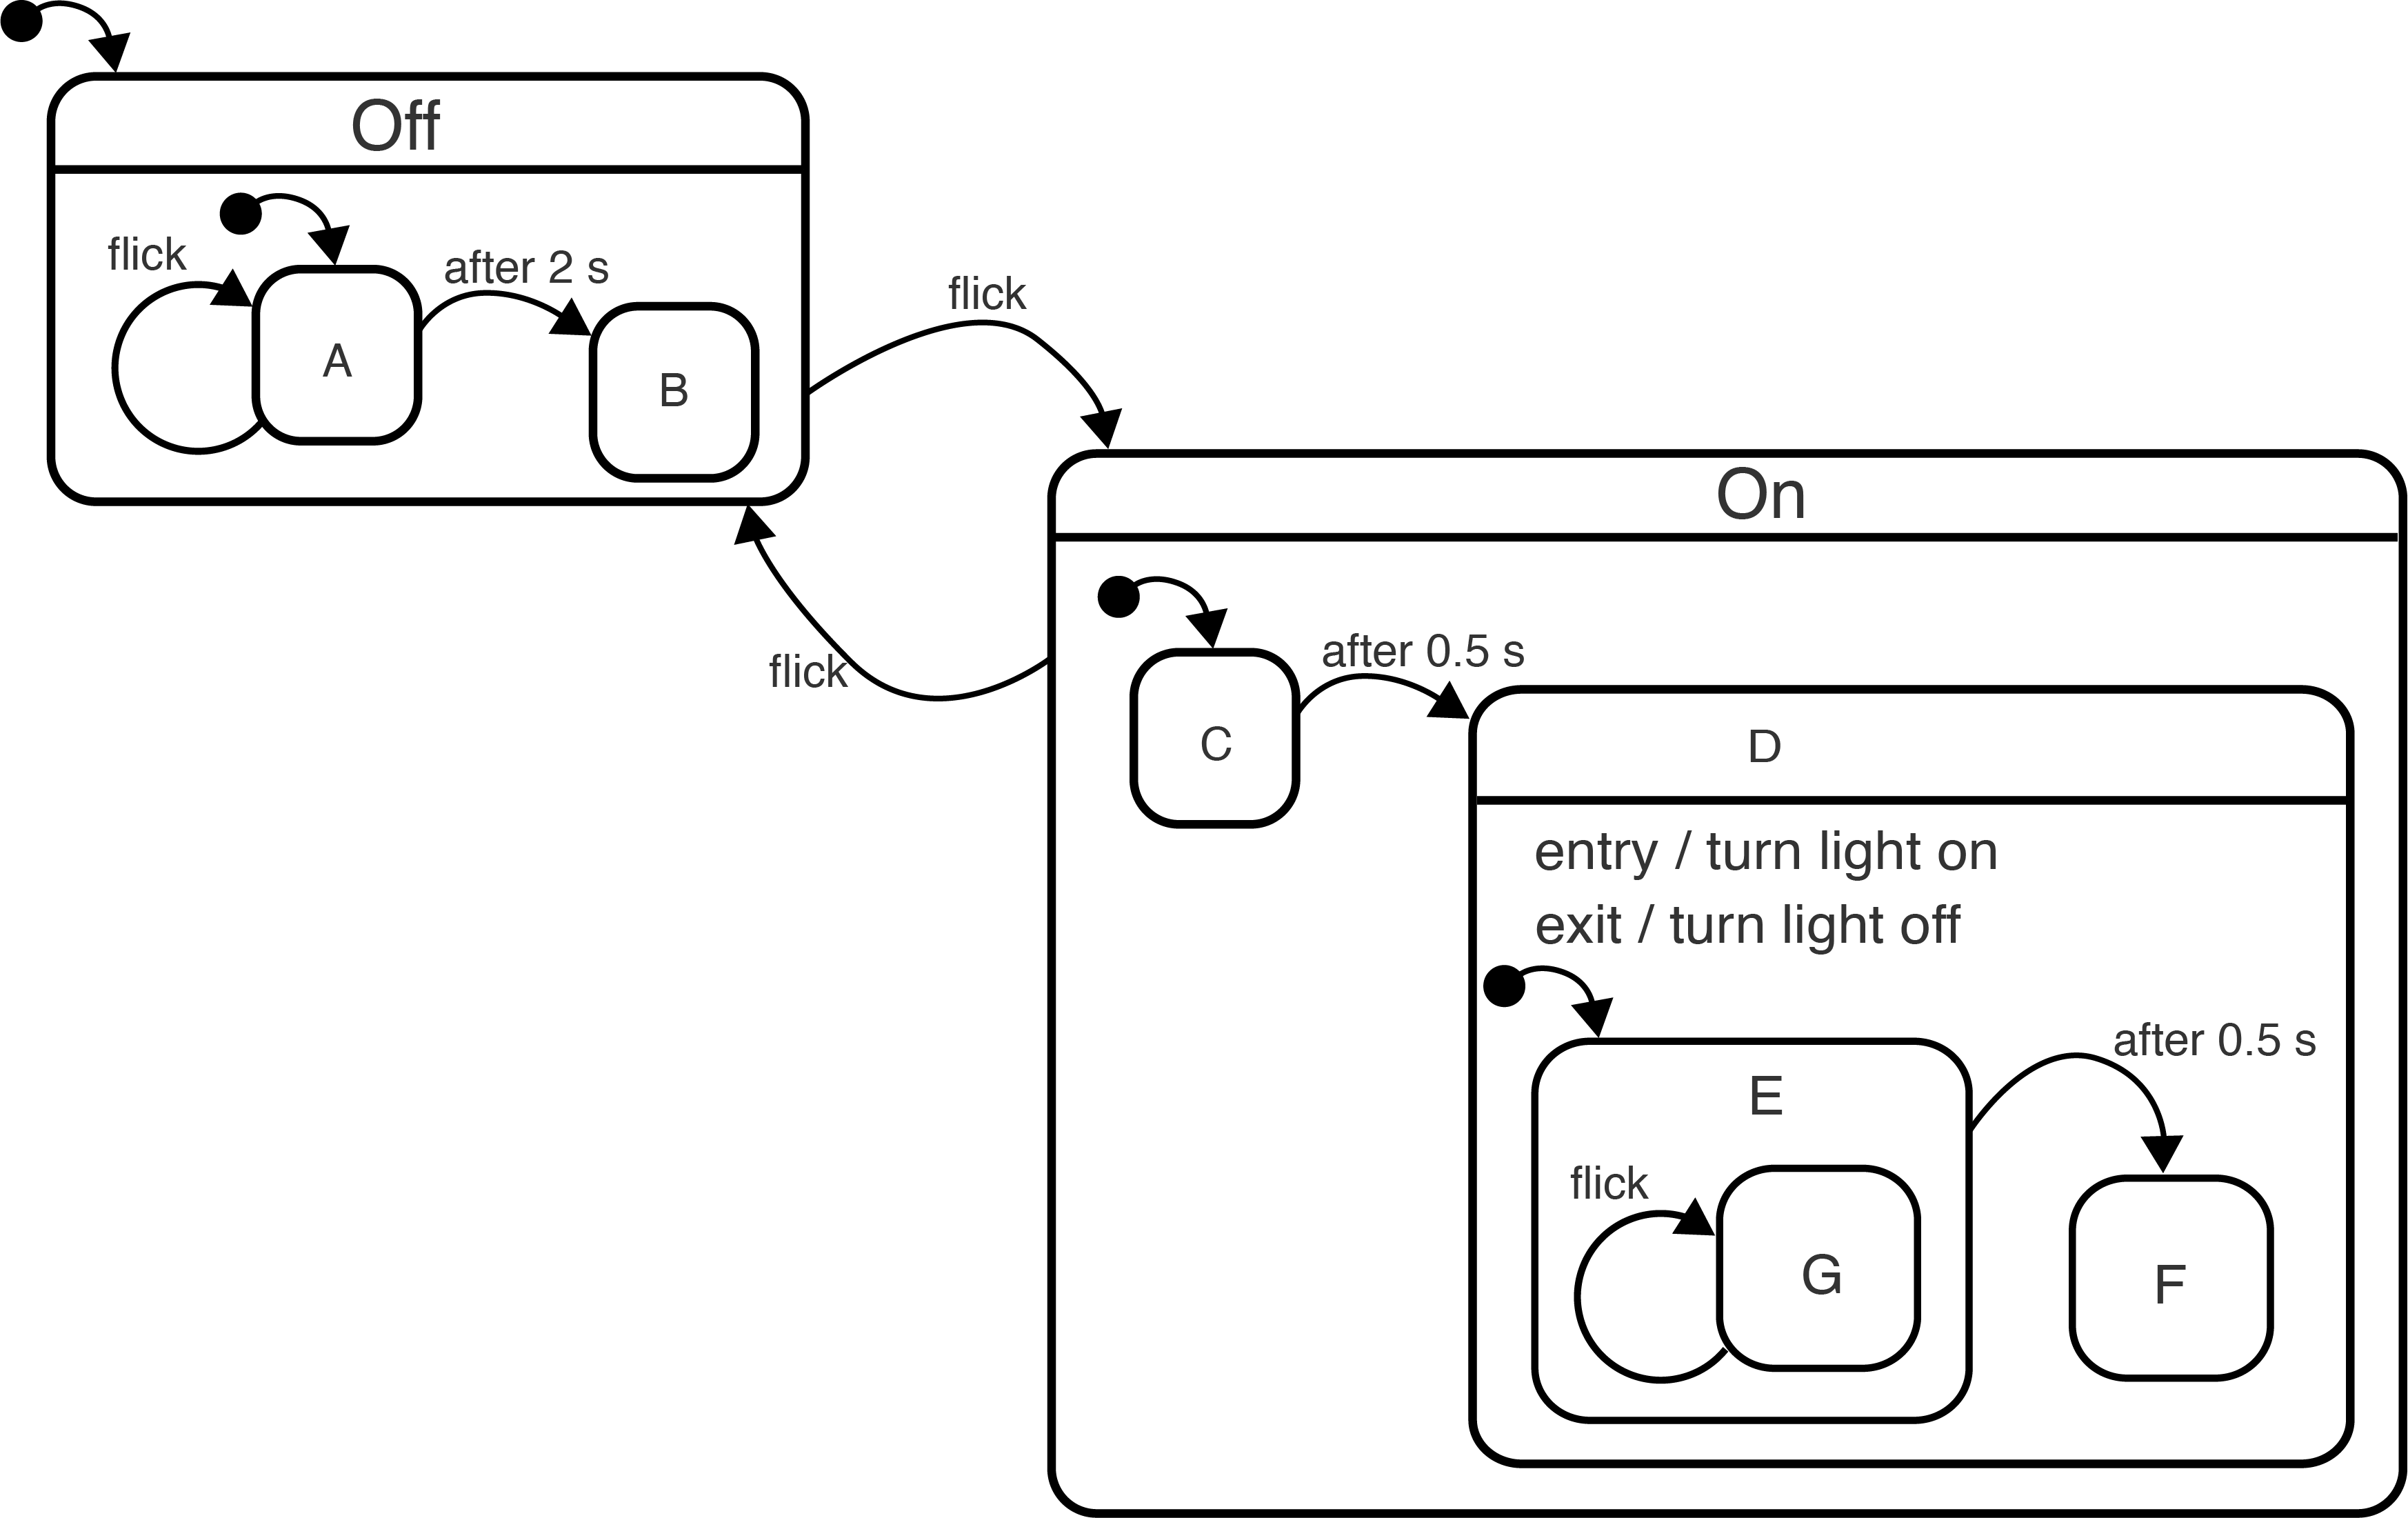
\includegraphics[width=\linewidth]{../assets/images/on-off-delayed-exit-1.png}
\emph{``When you flick a lightswitch, wait 0.5 seconds before turning
the light on, then once it's on wait 0.5 seconds before being able to
turn it back off again. When you flick it off, wait 2 seconds before you
can turn it on again.}

They have an extensive set of documents that defend the consistency and
readability of statecharts on their
\href{https://statecharts.dev/}{homepage}, and my point here is not to
disagree with them. My point is instead that tools that aspire to the
status of generalized infrastructure can't ask people to dramatically
change the way they think about and do science. There are many possible
realizations of this task, and each is more or less natural to every
person.

The problem here is really one of emphasis, BEADL seeks to solve
problems with inconsistencies in terminology by standardizing them, and
in order to do that seeks to standardize the syntax for specifying
experiments.

This means of standardization has many attractive qualities and is being
led by very capable researchers, but I think the project is illustrative
of how the differing constraints of different systems and differing
goals of different approaches influence the possible space of tooling.
Analysis tasks are often asynchronous, where the precise timing of each
node's completion is less important than the path dependencies between
different nodes be clearly specified. Analysis tasks often have a
clearly defined set of start, end, and intermediate cache points, rather
than branching or cyclical decision paths that change over multiple
timescales. Statecharts are a hierarchical abstraction of finite state
machines, the primary advantage of which is that they are better able to
incorporate continuous and history-dependent behavior, which causes
state explosion in traditional finite-state machines.

\href{https://docs.auto-pi-lot.com}{Autopilot} \cite{saundersAutopilotAutomatingBehavioral2019}  approaches the problem
differently by avoiding standardizing \emph{experiments} themselves,
instead providing smaller building blocks of experimental tools like
hardware drivers, data transformations, etc. and emphasizing
understanding their use in \emph{context.} This approach sacrifices some
of the qualities of a standardized system like being a logically
complete or having guaranteed interoperability of terms in order to
better support integrating with existing work patterns and making work
cumulative. It is a bit more humble: because we can't possibly predict
the needs and limitations of a totalizing system, we split the problem
along the different domains of tools and give facility for describing
how they are used together.

For concrete example, we might imagine the lightswitch in an
autopilot-like framework like this:

\begin{Shaded}
\begin{Highlighting}[]
\ImportTok{from}\NormalTok{ autopilot.hardware.gpio }\ImportTok{import}\NormalTok{ Digital\_Out}
\ImportTok{from}\NormalTok{ time }\ImportTok{import}\NormalTok{ sleep}
\ImportTok{from}\NormalTok{ threading }\ImportTok{import}\NormalTok{ Lock}

\KeywordTok{class}\NormalTok{ Lightswitch(Digital\_Out):}
  \KeywordTok{def} \FunctionTok{\_\_init\_\_}\NormalTok{(}\VariableTok{self}\NormalTok{,}
\NormalTok{    off\_debounce: }\BuiltInTok{float} \OperatorTok{=} \DecValTok{2}\NormalTok{,}
\NormalTok{    on\_delay:     }\BuiltInTok{float} \OperatorTok{=} \FloatTok{0.5}\NormalTok{,}
\NormalTok{    on\_debounce:  }\BuiltInTok{float} \OperatorTok{=} \FloatTok{0.5}\NormalTok{):}
    \CommentTok{"""}
\CommentTok{    Args:}
\CommentTok{      off\_debounce (float): }
\CommentTok{        Time (s) before light can be turned back on}
\CommentTok{      on\_delay (float): }
\CommentTok{        Time (s) before light is turned on}
\CommentTok{      on\_debounce (float): }
\CommentTok{        Time (s) after turning on that light can\textquotesingle{}t be turned off}
\CommentTok{    """}
    \VariableTok{self}\NormalTok{.off\_debounce }\OperatorTok{=}\NormalTok{ off\_debounce}
    \VariableTok{self}\NormalTok{.on\_delay     }\OperatorTok{=}\NormalTok{ on\_delay}
    \VariableTok{self}\NormalTok{.on\_debounce  }\OperatorTok{=}\NormalTok{ on\_debounce}

    \VariableTok{self}\NormalTok{.on }\OperatorTok{=} \VariableTok{False}
    \VariableTok{self}\NormalTok{.lock }\OperatorTok{=}\NormalTok{ Lock()}

  \KeywordTok{def}\NormalTok{ switch(}\VariableTok{self}\NormalTok{):}
    \CommentTok{\# use a lock to make sure if}
    \CommentTok{\# called while waiting, we ignore it}
    \ControlFlowTok{if} \KeywordTok{not} \VariableTok{self}\NormalTok{.lock.acquire():}
      \ControlFlowTok{return}

    \CommentTok{\# if already on, switch off}
    \ControlFlowTok{if} \VariableTok{self}\NormalTok{.on: }
      \VariableTok{self}\NormalTok{.on }\OperatorTok{=} \VariableTok{False}
\NormalTok{      sleep(}\VariableTok{self}\NormalTok{.off\_debounce)}

    \CommentTok{\# otherwise switch on}
    \ControlFlowTok{else}\NormalTok{: }
\NormalTok{      sleep(}\VariableTok{self}\NormalTok{.on\_delay)}
      \VariableTok{self}\NormalTok{.on }\OperatorTok{=} \VariableTok{True}
\NormalTok{      sleep(}\VariableTok{self}\NormalTok{.on\_debounce)}

    \VariableTok{self}\NormalTok{.lock.release()}
\end{Highlighting}
\end{Shaded}

The terms \texttt{off\_debounce}, \texttt{on\_delay}, and
\texttt{on\_debounce} are certainly not part of a controlled ontology,
but we have described how they are used in the docstring and how they
are used is inspectable in the class itself.

The difficulty of a controlled ontology for experimental frameworks is
perhaps better illustrated by considering a full experiment. In
Autopilot, a full experiment can be parameterized by the \texttt{.json}
files that define the task itself and the system-specific configuration
of the hardware. An
\href{https://gist.github.com/sneakers-the-rat/eebe675326a157df49f66f62c4e33a6e}{example
task} from our lab consists of 7 behavioral shaping stages that
introduce the animal to different features of a fairly typical auditory
categorization task, each of which includes the parameters for at most
12 different stimuli per stage, probabilities for presenting lasers,
bias correction, reinforcement, criteria for advancing to the next
stage, etc. So just for one relatively straightforward experiment, in
one lab, in one subdiscipline, there are \textbf{268 parameters} --
excluding all the default parameters encoded in the software.

The way Autopilot handles various parameters are part of set of layers
of abstraction that separate idiosyncratic logic from the generic form
of a particular \texttt{Task} or \texttt{Hardware} class. The general
structure of a two-alternative forced choice task is shared across a
number of experiments, but they may have different stimuli, different
hardware, and so on. Autopilot \texttt{Task}s use abstract references to
classes of hardware components that are required to run them, but
separates their implementation as a system-specific configuration so
that it's not necessary to have \emph{exactly the same} components
plugged into \emph{exactly the same} GPIO pins, etc. Task parameters
like stimuli, reward timings, etc. are similarly split into a separate
task parameterization that both allow \texttt{Task}s to be generic and
make provenance and experimental history easier to track. \texttt{Task}
classes can be subclasses to add or modify logic while being able to
reuse much of the structure and maintain the link between the root task
and its derivatives --- for example
\href{https://github.com/auto-pi-lot/autopilot-plugin-wehrlab/blob/9cfffcf5fe1886d25658d4f1f0c0ffe41c18e2cc/gap/nafc_gap.py\#L13-L49}{one
task we use} that starts a continuous background sound but otherwise is
the same as the root \texttt{Nafc} class. The result of these points of
abstraction is to allow exact experimental replication on inexactly
replicated experimental apparatuses.

In contrast, workflows in Bonsai \cite{lopesBonsaiEventbasedFramework2015a, lopesNewOpenSourceTools2021} ,
another very popular and very capable experimental tool,
\href{https://github.com/bonsai-rx/bonsai-examples/blob/cbc2c1decc11e1dc1df920421ef88a16fd2e184c/RoiTrigger/RoiTrigger.bonsai}{combine
the pattern of nodes} that constitute an experiment with idiosyncratic
parameters like a
\href{https://github.com/bonsai-rx/bonsai-examples/blob/cbc2c1decc11e1dc1df920421ef88a16fd2e184c/RoiTrigger/RoiTrigger.bonsai\#L76-L85}{crop
bounding box}. To be clear, I love Bonsai, and this kind of workflow
reproducibility is a huge step up from the more common practice of
totally lab-specific code. The flat design of Bonsai is extremely useful
for prototyping and extends through to complex experiments, but would
have a hard time being able to support generalizable and reusable
software classes for basic experimental operations, as well as creation
and negotiation over experimental terminology.

We can imagine extending the abstract specification of experimental
parameters, hardware requirements, and so on to work with our federated
naming system to overcome the challenges to standardizing. First, we can
imagine being able to make explicit declarations about the relationship
between our potentially very local terminology. Here we can declare our
\texttt{Lightswitch} object and 1) link its \texttt{on\_delay} to our
friend \texttt{@rumbly}'s object that implements the same thing as
\texttt{on\_latency}, and 2) link it to a standardized \texttt{Latency}
term from
\href{https://scicrunch.org/scicrunch/interlex/view/ilx_0106040\#annotations}{interlex},
but since that term is for time elapsed between a stimulus and
behavioral response in a psychophysical context, it's only a partial
match.

\begin{verbatim}
<#Lightswitch>
  a @autopilot.hardware.Digital_Out

  param on_delay
    @skos:exactMatch @rumbly:LED:on_latency
    @skos:nearMatch @interlex:Latency

  providedBy
    @git:repository ...
    @python:class ...
\end{verbatim}

Further, since our experimental frameworks are intended to handle off
the shelf parts as well as our potentially idiosyncratic lightbulb
class, we can link many implementations of a hardware controlling class
to the product itself. Take for example the
\href{https://docs.auto-pi-lot.com/en/latest/hardware/i2c.html\#autopilot.hardware.i2c.I2C_9DOF}{I2C\_9DOF}
class that controls a 9 degree of freedom motion sensor from
\href{https://www.sparkfun.com/products/13944}{Sparkfun} where we both
indicate the specific part itself as well as the generic \texttt{ic}
that it uses:

\begin{verbatim}
<#I2C_9DOF>
  @autopilot.controlsHardware
    @sparkfun:13944
    @ic:LSM9DS1
\end{verbatim}

This hints at the first steps of a system that would make our technical
work more cumulative, as it is then easy to imagine being able to search
for all the different implementations for a given piece of hardware.
Since the \texttt{@sparkfun:13944} element can in turn specify
properties like being an inertial motion sensor, this kind of linking
becomes powerful very quickly to make bridges that allow similar work to
be discovered and redeployed quickly.

We can also extend our previous connection between a dataset and the
results of its analysis to also include the tools that were used to
collect it. Say we want to declare the
\href{https://gist.github.com/sneakers-the-rat/eebe675326a157df49f66f62c4e33a6e}{example
experiment} above, and then extend our
\texttt{\textless{}\#project-name\textgreater{}} project to, also above,
to reference it:

\begin{verbatim}
<#example-experiment>
  a @autopilot:protocol

  level @autopilot:freeWater
    reward
      type mL
      value 5
    graduation 
      a @autopilot:graduation:ntrials
      n_trials 200

  level @autopilot:Nafc
    stim
      @autopilot:stim:sound:Tone
        frequency 5000
        duration 100

  ...

  @autopilot:prefs
    @jonny:Lightswitch
      on_delay 1

<#project-name-2>
  a @jonny:project-name
  collectedBy @jonny:example-experiment
\end{verbatim}

So while we sacrifice the direct declaration of standardized terminology
and syntax, we gain the potential for a much denser and richer
expressive structure for our experiments. Instead of a single
authoritative dictionarylike meaning for a term, we instead appreciate
it in the context of its use, linked to the code that implements it as
well as the data it produces and the kinds of arguments that are made
with different analysis chains. Of course there is no intrinsic conflict
with this kind of freewheeling system and controlled vocabularies and
syntaxes: in this system, they can be one of many means of expression
rather than need to be singular sources of truth that depend on wide
adoption. While individual instances of uncontrolled vocabularies might
mean chaos, when they are integrated in a system of practice we get
something much wilder but also more intricate, beautiful, and useful.

As in the case of analytical tools, the role of the experimental
frameworks is also to make interacting with the rest of the system
easier and doesn't involve manually editing a lot of metadata. For
example, currently autopilot \texttt{Task}s ask users to declare
collected data as a \href{https://www.pytables.org/}{pytables} \cite{altedPyTablesProcessingAnalyzing2003}  datatypes like
\texttt{target\ =\ tables.StringCol(1)} to record whether a target is
\texttt{\textquotesingle{}L\textquotesingle{}} or
\texttt{\textquotesingle{}R\textquotesingle{}}. If instead it was
capable of specifying a Neurodata Without Borders data type like
\texttt{target\ =\ \textquotesingle{}@nwb:behavior:BehavioralEvents\textquotesingle{}},
then it would be possible to directly output to a standardized format,
potentially also automatically creating a
\href{https://pynwb.readthedocs.io/en/stable/pynwb.behavior.html\#pynwb.behavior.BehavioralEpochs}{\texttt{BehavioralEpochs}}
container or other data that are implied but otherwise have to be
explicitly created. Autopilot already automatically tracks the entire
behavioral history of an experimental subject, so we can also imagine it
being able to automatically create a \texttt{@analysis:project} object
described above that groups together multiple datasets that connected
them to an analysis pathway. So in this example the elusive workflow
where experimental data is automatically scooped up and incrementally
analyzed that is typically a hard-won engineering battle within a single
lab would become the normal mode of using the system.

The experimental framework described so far could solve some of the
software challenges of doing experiments by providing a system for
extending a set of reusable classes that can be combined into
experiments and linked together, but we haven't described anything to
address the rest of the contextual knowledge of practical scientific
work. We also haven't described any sort of governance or development
system that makes these packages anything more than ``some repository on
GitHub somewhere'' with all the propensity to calcify into fiefdoms that
those entail. This leads us back to a system of communication, the
central piece of missingness that we have been circling around the whole
piece. If you'll allow me one more delay, I want to summarize the system
so far before finally arriving there.


\end{multicols}


\hypertarget{abstraction-protocol-design}{%
\subsubsection{Abstraction \& Protocol
Design}\label{abstraction-protocol-design}}


\begin{multicols}{2}


This section should be split back up s.t. the parts specific to
analysis/experimental tools are at the ends of those sections, and we
should move the discussion about layers of abstraction congealing into a
protocol in the end in the practical implementation section. I'm leaving
this here until I have time to do that, but for now you probably want to
skip to the next section :)

Though there are many similarities between the three domains of data,
analytical, and experimental tools, the different constraints each
impose on a generalizable framework for integration and interoperability
are instructive. Each requires a careful consideration of the
\emph{layers of abstraction} needed to maintain the modularity of the
system --- this is an elemental feature of any protocol design. What are
the minimal affordances needed to implement a wide array of systems and
technologies within each domain? By being careful with specifying
abstraction, when considered together, the linked system described so
far represents a powerful step towards \emph{collectivizing the
scientific state of the art.}

There are three primary layers of abstraction in the analysis system
described: the interface between the metadata description of a node and
the code that implements it, the separation of individual nodes and a
notion of a combined workflow, and perhaps more subtly the separation of
the data applied to the workflow and the workflow itself.

!! while the analysis system seeks to make multiple software packages
and environments be interoperable together, the experimental framework
makes no such attempt. !! the need for careful timing and adaptation to
individual systems leaves integration for the implementing codebases.

\begin{itemize}
\item
  First, the markup description of the node gives us abstraction from
  programming language and implementation. This lets us do stuff like
  use multiple tools with competing environmental needs, adapt to
  multiple versions of the code markup as it develops, etc. Note the
  interaction with the rest of the metadata system: because we required
  a particular type of data file, and that link should provide us some
  means of opening/instantiating the file with dependencies, we didn't
  need to write loading code. Since it's in a linked system, someone
  could override the implementation of my node -- say someone comes up
  with a faster means of binning, then they just inherit from my node
  and replace the reference to the code. Boom we have cumulative and
  linked development.
\item
  The separation of the node from the workflow means that the node can
  be shared and swapped and reintegrated easily, dramatically reducing
  the brittleness of the systme. Since there is no restriction on what
  constitutes a node, though, there's no reason that nodes can't be
  either made massive, like putting a whole library in the process
  method, or be packaged up together. If we made the argument and method
  names recursive between the workflow and the node objects then tooling
  could automatically traverse multiple layers of node/workflow
  combinations at different levels of abstraction. This being a
  schematic description means that there can be multiple ``workflow
  runner'' packages that eg. distribute the task across a billion
  supercomputers or not.
\item
  Finally, the separation between the data applied and the workflow
  itself are very cool indeed given our linked and namespaced system. My
  workflow effectively constitutes ``an unit of analysis.'' I have
  linked my data to this unit of analysis. Play out the permutations:

  \begin{itemize}
  
  \item
    I can see all the analyses that this particular pipeline has been
    applied to. Since it is embedded within the same federated system as
    our schema system, I can draw and connect semantic links to similar
    analysis pipelines as well as pipeline/data combinations.
  \item
    I can see all the different analyses that have been applied to my
    data: if my data is analyzed a zillion different times, in a zillion
    different combinations of data, I effectively get a ``multiverse
    analysis'' (cite dani) and we get to measure robustness of my data
    for free. It also gets to live forever and keep contributing to
    problems !! and i also get credited for it automatically by golly!
    This also applies on cases like cross-validation or evaluating
    different models on the same data: the versioning of it falls out
    naturally. Also since model weights would be an input to an analysis
    chain, we also get stuff like DLC's model zoo where we can share
    different model weights, combine them, and have a cumulative library
    of pretrained models as well!
  \item
    being able to look across the landscape\ldots{} we start being able
    to actually really make cumulative progress on best practices. A
    common admonishment in cryptographically-adjacent communities is to
    ``never roll your own crypto,'' because your homebrew crypto library
    will never be more secure than reference implementations that have
    an entire profession of people trying to expose and patch their
    weaknesses. Bugs in analysis code that produce inaccurate results
    are inevitable and rampant \cite{millerScientistNightmareSoftware2006, soergelRampantSoftwareErrors2015, eklundClusterFailureWhy2016a, bhandarineupaneCharacterizationLeptazolinesPolar2019} , but
    impossible to diagnose when every paper writes its own pipeline. A
    common analysis framework would be a single point of inspection for
    bugs, and facilitate re-analysis and re-evaluation of affected
    results after a patch.
  \item
    looking forward, we might imagine our project object being linked to
    a DOI\ldots{} we'll get there.
  \end{itemize}
\end{itemize}

!! this is all extraordinarily reproducible because even though I have
my portable markup description of the analysis, I can just refer to it
by name in my paper (ya ya need some content based hash or archive but
you get the idea)

!! since we have a bunch of p2p systems all hooked up with
constantly-running daemons, to compete with the compute side of cloud
technology we also should implement a voluntary compute grid akin to
\href{https://foldingathome.org/}{Folding@Home}. This has the same
strawmen and answers to them as the peer-to-peer system --- no i'm not
saying everyone puts their shitty GPU up, but it lets us combine the
resources that are present at an institutional level and makes a very
cheap onramp for government-level systems to be added to the mix.

!! this is all very exciting, and we can immediately start digging
towards larger scientific problems, eg. what it would mean for the file
drawer problem and publication bias when the barriers to analyzing data
are so low you don't even need to write the null result: the data is
already there, semantically annotated and all. Dreams of infinite
meta-analyses across all data and all time, but hold your horses! We
don't get magic for free, we haven't talked about the community systems
yet that are the unspoken glue of all of this!!

The category distinction between experimental and analytical tools is,
of course, a convenient ordering fiction for the purpose of this piece.
Autopilot is designed to make it easy to integrate other tools, and \cite{kaneRealtimeLowlatencyClosedloop2020} 

!! so in parallel to our linking scheme is the development patterns that
we use. The linking system is general enough for allcomers, and it
implies the patterns of linkage that should exist, but they then need to
be implemented. Much like desire pathways though, the frequent co-use of
different tools gives a good idea about the direction that development
should go. So the systems work reciprocally: metadata linking system
connect ideas and tools, and can

!! these are examples of what happens when you relax the demanding parts
of an exact ontology/knowledge graph -- we don't guarantee computability
across the graph itself, there's no way to automatically whiz
uncritically across all datasets in the system, but as we have seen
that's also not really true of the other systems either, to the degree
that it's desirable at all. Instead of having formal guarantees on the
graph, we can design tools that automate certain parts of the
interaction with the system to actually make our jobs easier. By being
very permissive, we let the desire paths of tool use form. This is a
very literal example of the `empower people, not systems' principle.

!! reciprocally, we can also imagine the reverse: being able to develop
metadata structures that are then code generators for tools that have a
sufficiently sophisticated API -- for example remember how we said
Bonsai might have a hard time making generalizable behavioral tasks/etc?
Imagine if someone made a code compilation tool that allowed people to
declare abstract structures that could then be reusably reparameterzied
that autocreated a bonsai workflow? In the same way that the metadata
system can be used for \emph{storage} of existing work, it can also be
used to create abbreviate and abstract constructs for \emph{use} with
other tools.

!! continue the example of needing to select within datasets instead of
metadata from federation section.

To take stock:

We have described a system of three component modalities: \textbf{data,
analytical tools, and experimental tools} connected by a \textbf{linked
data} layer. We started by describing the need for a
\textbf{peer-to-peer} data system that makes use of \textbf{data
standards} as an onramp to linked metadata. To interact with the system,
we described an identity-based linked data system that lets individual
people declare linked data resources and properties that link to
\textbf{content addressed} resources in the p2p system, as well as
\textbf{federate} into multiple larger organizations. We described the
requirements for \textbf{DAG-based analytical frameworks} that allow
people to declare individual nodes for a processing chain linked to
code, combine them into workflows, and apply them to data. Finally, we
described a design strategy for \textbf{component-based experimental
frameworks} that lets people specify experimental metadata, tools, and
output data.

This system as described is a two-layer system, with a few different
domains linked by a flexible metadata linking layer. The metadata system
as described is not merely \emph{inert} metadata, but metadata linked to
code that can \emph{do something} --- eg. specify access permissions,
translate between data formats, execute analayis workflows, parameterize
experiments, etc. Put another way, we have been attempting to describe a
system that \emph{embeds the act of sharing and curation in the practice
of science.} Rather than a thankless post-hoc process, the system
attempts to provide a means for aligning the daily work of scientists so
that it can be cumulative and collaborative. To do this, we have tried
to avoid rigid specifications of system structure, and instead described
a system that allows researchers to pluralistically define the structure
themselves.

!! Now we need to consider the social tools needed to communicate
within, negotiate over, and govern the system.


\end{multicols}


\hypertarget{shared-knowledge}{%
\subsection{Shared Knowledge}\label{shared-knowledge}}


\begin{multicols}{2}
 The remaining set of problems implied by the
infrastructural system sketched in the preceding sections is the
\emph{communication} and \emph{organization} systems that make up the
interfaces to maintain and use it. We can finally return to some of the
breadcrumbs laid before: the need for negotiating over distributed and
conflicting data schema, for incentivizing and organizing collective
labor, and ultimately for communicating scientific results.

The communication systems that are needed double as \emph{knowledge
organization} systems. Knowledge organization has the rosy hue of
something that might be uncontroversial and apolitical --- surely
everyone involved in scientific communication wants knowledge to be
organized, right? The reality of scientific practice might give a hint
at our naivete. Despite being, in some sense, itself an effort to
organize knowledge, \emph{scientific results effectively have no system
of organization.} There is no means of, say, ``finding all the papers
about a research question.'' The problem is so fundamental it seems
natural: the usual methods of using search engines, asking around on
Twitter, and chasing citation trees are flex tape slapped over the
central absence of a system for formally relating our work as a shared
body of knowledge.

Information capitalism, in its terrifying splendor, here too pits
private profit against public good. Analogously to the necessary
functional limitations of SaaS platforms, artificially limiting
knowledge organization opens space for new products and profit
opportunities. In their 2020 shareholder report, RELX, the parent of
Elsevier, lists increasing the number of journals and papers as a
primary means of increasing revenue \cite{RELXAnnualReport2020} .
In the next breath, they describe how ``in databases \& tools and
electronic reference, representing over a third of divisional\footnote{RELX
  is a huge information conglomerate, and scientific publication is just
  one division.} revenue, we continued to drive good growth through
content development and enhanced machine learning {[}ML{]} and natural
language processing {[}NLP{]} based functionality.''

What ML and NLP systems are they referring to? The 2019 report is a bit
more revealing (emphases mine):

\begin{quote}
Elsevier looks to enhance quality by building on its premium brands and
\textbf{grow article volume} through \textbf{new journal launches,} the
expansion of open access journals and growth from emerging markets; and
add value to core platforms by implementing capabilities such as
\textbf{advanced recommendations on ScienceDirect and social
collaboration through reference manager and collaboration tool
Mendeley.}

\textbf{In every market, Elsevier is applying advanced ML and NLP
techniques} to help researchers, engineers and clinicians perform their
work better. For example, in research, ScienceDirect Topics, a free
layer of content that enhances the user experience, uses \textbf{ML and
NLP techniques to classify scientific content and organise it
thematically,} enabling users to get faster access to relevant results
and related scientific topics. The feature, launched in 2017, is proving
popular, generating 15\% of monthly unique visitors to ScienceDirect via
a topic page. \textbf{Elsevier also applies advanced ML techniques that
detect trending topics per domain,} helping researchers make more
informed decisions about their research. \textbf{Coupled with the
automated profiling and extraction of funding body information from
scientific articles,} this process supports the whole researcher
journey; from planning, to execution and funding. \cite{RELXAnnualReport2019} 
\end{quote}

Reading between the lines, it's clear that the difficulty of finding
research is a feature, not a bug of their system. Their explicit
business model is to increase the number of publications and sell
organization back to us with recommendation services. The recommendation
system might be free*, but the business is to develop dependence to sell
ad placement --- which they proudly describe as looking very similar to
their research content \cite{springernatureBrandedContent, elsevier360AdvertisingSolutions} .

It gets more sinister: Elsevier sells multiple products to recommend
`trending' research areas likely to win grants, rank scientists, etc.,
algorithmically filling a need created by knowledge disorganization. The
branding varies by audience, but the products are the same. For
pharmaceutical companies
\href{https://www.elsevier.com/solutions/professional-services/drug-design-optimization\#opportunity}{``scientific
opportunity analysis''} promises custom reports that answer questions
like ``Which targets are currently being studied?'' ``Which experts are
not collaborating with a competitor?'' and ``How much funding is
dedicated to a particular area of research, and how much progress has
been made?'' \cite{elsevierDrugDesignOptimization} . For
academics,
\href{https://www.elsevier.com/solutions/scival/features/topic-prominence-in-science\#how}{``Topic
Prominence in Science''} offers university administrators tools to
``enrich strategic research planning with portfolio overviews of their
own and peer institutions.'' Researchers get tools to ``identify experts
and potential cross-sector collaborators in specific Topics to
strengthen their project teams and funding bids and identify Topics
which are likely to be well funded.'' \cite{elsevierTopicProminenceScienceb} 

These tools are, of course, designed for a race to the bottom --- if my
colleague is getting an algorithmic leg up, how can I afford not to?
Naturally only those labs that \emph{can} afford them and the costs of
rapidly pivoting research topics will benefit from them, making yet
another mechanism that reentrenches scientific inequity for profit.
Knowledge disorganization, coupled with a little surveillance capitalism
that monitors the activity of colleagues and rivals \cite{brembsReplacingAcademicJournals2021} , has given publishers powerful
control over the course of science, and they are more than happy to ride
algorithmically amplified scientific hype cycles in fragmented research
bubbles all the way to the bank.

The consequences are hard to overstate. In addition to literature search
being an unnecessarily huge sink of time and labor, science operates as
a wash of tail-chasing results that only rarely seem to cumulatively
build on one another. The need to constantly reinforce the norm that
purposeful failure to cite prior work is research misconduct is itself a
symptom of how engaging with a larger body of work is both extremely
labor intensive and \emph{strictly optional} in the communication regime
of journal publication. Despite the profusion of papers, by some
measures progress in science has slowed to a crawl as the long tail of
papers with very few citations grows ever longer \cite{chuSlowedCanonicalProgress2021} .

While Chu and Evans correctly diagnose \emph{symptoms} of knowledge
disorganization like the need to ``resort to heuristics to make
continued sense of the field'' and reliance on canonical papers, by
treating the journal model as a natural phenomenon and citation as the
only means of ordering research, they misattribute root \emph{causes.}
The problem is not people publishing \emph{too many papers,} or a
\emph{breakdown of traditional publication hierarchies,} but the
\emph{profitability of knowledge disorganization.} Their prescription
for ``a clearer hierarchy of journals'' misses the role of organizing
scientific work in journals ranked by prestige, rather than by the
content of the work, as a potentially major driver of extremely skewed
citation distributions. It also misses the publisher's stated goal of
pushing algorithmic paper recommendations, as there is nothing
recommendation algorithms love recommending more than things that are
alreaady popular. Without diagnosing knowledge disorganization as a core
part of the business model of scientific publishers, we can be led to
prescriptions that would make the problem worse.

!! Another impact of the arcanity of scientific knowledge organization
is that it is effectively impenetrable to people that aren't domain
experts. Why is trust in science so low right now? one contributor is
that they have no idea what the hell we do or how different domains of
knowledge have evolved. (cite cold war peer review and journals paper)

!! Practically, this makes the quality of scientific literature
constantly in question. Each paper effectively exists as an island, and
engagement with prior literature is effectively optional (outside the
minimum bar set by the 3-5 additional private peer reviewers, each with
their own limited scope and conflicting interests). Forensic
peer-reviewers have been ringing the alarm bell, saying that there is
``no net'' to bad research \cite{heathersRealScandalIvermectin2021} , and brave and highly-skilled investigators like
\href{https://scienceintegritydigest.com/}{Elisabeth Bik} have found
thousands of papers with evidence of purposeful manipulation \cite{shenMeetThisSuperspotter2020, bikPrevalenceInappropriateImage2016} .
!! So our existing systems of communication and organization are
woefully inadequate for our needs, and don't serve the role of
guaranteeing consistency or reliability in research that they claim to.

It's hard to imagine an alternative to journals that doesn't look like,
well, journals. While a full treatment of the journal system is outside
the scope of this paper, the system we describe here renders them
\emph{effectively irrelevant} by making papers as we know them
\emph{unnecessary.} Rather than facing the massive collective action
problem of asking everyone to change their publication practices head
on, by reconsidering the way we organize the surrounding infrastructure
of science we can flank journals and replace them ``from below'' with
something qualitatively more useful.

Beyond journals, the other technologies of communication that have been
adopted out of need, though not necessarily design, serve as
\href{https://en.wikipedia.org/wiki/Desire_path}{desire paths} that
trace other needs for scientific communication. As a rough sample:
Researchers often prepare their manuscripts using platforms like Google
Drive, indicating a need for collaborative tools in perparation of an
idea. When working in teams, we often use tools like Slack to plan our
work. Scientific conferences reflect the need for federated
communication within subdisciplines, and we have adopted Twitter as a de
facto platform for socializing and sharing our work to a broader
audience. We use a handful of blogs and other sites like
\href{https://edspace.american.edu/openbehavior/}{OpenBehavior} \cite{whiteFutureOpenOpenSource2019} ,
\href{https://open-neuroscience.com/}{Open Neuroscience}, and many
others to index technical knowledge and tools. Finally we use sites like
\href{https://pubpeer.com}{PubPeer} and ResearchGate for comment and
criticism.

These technologies point to a few overlapping and not altogether binary
axes of communication systems. !! make this a table? with technological
examples for each.

\begin{itemize}

\item
  \textbf{Durable vs Ephemeral} - journals seek to represent information
  as permanent, archival-grade material, but scientific communication
  also necessarily exists as wholly contextual, temporally specific
  snapshots.
\item
  \textbf{Structured vs Chronological} - scientific communication both
  needs to present itself as a structured basis of information with
  formal semantic linking, but also needs the chronological structure
  that ties ideas to their context. This axis is a gradient from formal
  ontologies, through intermediate systems like forums with hierarchical
  topic structure that embeds a feed, to the purely chronological
  feed-based social media systems.
\item
  \textbf{Messaging vs Indexing} - Communication can be person-to-person
  or person-to-group messaging with defined senders and recipients, or
  intended as a generalizable category of objects. This ranges from
  entirely-specific DMs through domain-specific tool indexes like
  OpenBehavior through the uniform indexing of Wikipedia.
\item
  \textbf{Public vs.~Private} - Communication can be composed of
  entirely private notes to self, through communication in a lab,
  collaboration group, discipline, and landing in the entirely public
  realm of global communication.
\item
  \textbf{Formal vs.~Informal} - Journal articles and encyclopedia-bound
  writing that conforms to a particular modality of expression vs.~a
  vernacular style intended to communicate with people outside the
  jargon culture.
\end{itemize}

!! There are many tunnels of internet history that have traced different
parts of these axes, but particularly relevant here are the overlapping
histories of early wikis, wikipedia, the semantic web, and activitypub.
This is a knotty and tangled history, so I am not attempting a full
recounting, but will be selectively telling the story to motivate the
kinds of tools we need.

\hypertarget{the-wiki-way}{%
\subsubsection{The Wiki Way}\label{the-wiki-way}}

x

current status - our current systems are largely journals and
conferences, but as evidenced by the unfortunate but widescale adoption
of twitter, scientific communication naturally spans dispersed forms of
communication at different scales of formality, length, public
engagement, etc. - when we go to organize ourselves, why is the best we
can do google docs and slack?

contextual knowledge needed - our limited systems of communication also
render large sections of needed scientific communication without venue.
The existing tools that \emph{do} give some means of sharing technical
knowledge are distinctly charity-driven, and don't confer the same type
of credit incentive that publications do.

!! important of ease of leaving
http://meatballwiki.org/wiki/RightToLeave

!! we've been tracing a distinction between the ability to express
fluidly the contents of our reality with developing platforms that sift
through it in an automated way, something that was an explicit cultural
division throughout the semantic web project \cite{swartzTechniquesMassCollaboration2006} , which Peter Norvig (director
of search at Google at the time) primarily attributes to user
incompetence \cite{lombardiGoogleExecChallenges2007} . On trust,
TBL says ``Berners-Lee agreed with Norvig that deception on the Internet
is a problem, but he argued that part of the Semantic Web is about
identifying the originator of information, and identifying why the
information can be trusted, not just the content of the information
itself.''

!! more techniques of communtiy growth
http://meatballwiki.org/wiki/RewardReputation

!! wikis work! but they can break when people get too much power!
http://www.aaronsw.com/weblog/whorunswikipedia

There simply isn't a place to have longform, thoughtful, durable
discussions about science. The direct connection between the lack of a
communcaition venue to the lack of a way of storing technical,
contextual knowledge is often overlooked. Because we don't have a place
to talk about what we do, we don't have a place to write down how to do
it. Science needs a communcation platform, but the needs and constraints
of a scientific communication platform are different than those
satisfied by the major paradigms of chatrooms, forums etc. By
considering this platform as another infrastructure project alongside
and integrated with those described in the previous sections, its form
becomes much clearer, and it could serve as the centerpiece of
scientific infrastructure.

!! importantly, should also have means of ingest for existing tools and
elements -- easy to import existing papers and citation trees, plugins
for existing data sharing systems.

!! description of its role as a schema resolution system -- currently we
implement all these protocols and standards in these siloed, centralized
groups that are inherently slow to respond to changes and needs in the
field. instead we want to give people the tools so that their the
knowledge can be directly preserved and acted on.

!! descrption of its role as a tool of scientific discussion --
integrated with the data server and standardized analysis pipelines, it
could be possible to have a discussion board where we were able to pose
novel scientific questions, answerable with transparent, interrogatable
analysis systems. Semantic linking makes the major questions in the
field possible to answer, as discussions are linked to one another in a
structured way and it is possible to literally trace the flow of
thought.

!! should trace the development of AP and the difficulty of doing these
things as a way to explaining the ecosystem and the different parts that
are needed in it: https://www.w3.org/TR/social-web-protocols/

\hypertarget{the-wiki-way-1}{%
\subsubsection{The Wiki Way}\label{the-wiki-way-1}}

\begin{quote}
So that's it --- insecure but reliable, indiscriminate and subtle, user
hostile yet easy to use, slow but up to date, and full of difficult,
nit-picking people who exhibit a remarkable community camaraderie.
Confused? Any other online community would count each of these
``negatives'' as a terrible flaw, and the contradictions as impossible
to reconcile. Perhaps wiki works because the other online communities
don't. \cite{leufWikiWayQuick2001a, -l, 329} 
\end{quote}

!! wiki cultural history stuff!! differences in wiki philosophy,
deletists vs not. !! meatball stuff on community maintenace, conflict
resolution,

!! also hints at the problems, difficulties with wiki culture

\begin{quote}
It's not too late to turn things around. Specs could be moved back into
the wiki until they're nearly done. Editors, instead of being
gatekeepers, could be helpful moderators. A clear process for making
controvertial decisions could be decided on. And the validator could
follow consensus instead of leading it. But do the people running the
show want this?

Standards bodies tread a fine line between organizations for the public
good and shelters for protecting collusion that would be otherwise
illegal under antitrust law. For the dominent vendors involved, the goal
is to give the illusion of openness while giving themselves full control
to enforce their will behind the scenes.

The IETF is a good example of this. Often lauded by the public as a
model of openness and and and freedom, the reality is that working group
chairs, appointed by a self-elected ruling board, get away with
declaring whatever they want (usually an inferior and difficult to
implement alternative) as ``rough consensus'', routinely ignoring
comments from the public and objections from working group members. One
working group (in charge of DNS extentsions) went so far as to censor
mail from working group members. The dictators running the IETF, when
informed, didn't seem to mind.

Is the same sort of thing at work in the Pie/Echo/Atom Project? It
appears so at first glance: Sam running the show from behind the scenes,
putting friends in charge of the specs (although that isn't what
actually happened). The lack of a dispute-resolution process only makes
things worse: when there's no clear guide on how to make decisions or
contributions, it's far from obvious how to challenge a decision Sam has
made. \cite{swartzSecretsStandards2003} 
\end{quote}

\begin{quote}
c2wiki is an exercise in dialogical methods. of laying bare the fact
that knowledge and ideas are not some truth delivered from On High, but
rather a social process, a conversation, a dialectic, between various
views and interests \cite{valentineC2wikiExerciseDialogical2021} 
\end{quote}

!! give the example of the autopilot wiki

!! contextual knowledge stuff in this section, theory wiki stuff in next
section

\begin{quote}
Two essential features coordinate this information to better serve our
organizational decision-making, learning, and memory. The first is our
constellation of Working Groups that maintain and distribute local,
specialized knowledge to other groups across the network. {[}\ldots{]} A
second, more emergent property is the subgroup of IBL researchers who
have become experts, liaisons, and interpreters of knowledge across the
network. These members each manage a domain of explicit records (e.g.,
written protocols) and tacit information (e.g., colloquialisms, decision
histories) that are quickly and informally disseminated to address
real-time needs and problems. A remarkable nimbleness is afforded by
this system of rapid responders deployed across our web of Working
Groups. However, this kind of internalized knowledge can be vulnerable
to drop-out when people leave the collaboration, and can be complex to
archive. An ongoing challenge for our collaboration is how to archive
both our explicit and tacit processes held in both people and places.
This is not only to document our own history but as part of a roadmap
for future science teams, whose dynamics are still not fully understood.
\cite{woolKnowledgeNetworksHow2020} 
\end{quote}

\cite{kamelboulosSemanticWikisComprehensible2009} 

!! Read and cite! \cite{classeDistributedInfrastructureSupport2017} 

!! \cite{goodSocialTaggingLife2009} 

!! wikibase can do federated SPARQL queries https://wikiba.se/ - and has
been used to make folksonomies https://biss.pensoft.net/article/37212/

!! lots of scientific wikis -
https://en.wikipedia.org/wiki/Wikipedia:WikiProject\_Molecular\_Biology/Genetics/Gene\_Wiki/Other\_Wikis
-
https://en.wikipedia.org/wiki/Wikipedia:WikiProject\_Molecular\_Biology/Genetics/Gene\_Wiki

!! bids is doing something like this https://nidm-terms.github.io/

!! interlex

\begin{quote}
The Semantic Web is about two things. It is about common formats for
integration and combination of data drawn from diverse sources, where on
the original Web mainly concentrated on the interchange of documents. It
is also about language for recording how the data relates to real world
objects. That allows a person, or a machine, to start off in one
database, and then move through an unending set of databases which are
connected not by wires but by being about the same thing.
https://www.w3.org/2001/sw/
\end{quote}

!! Semantic combination of databases in science are also not new \cite{cheungSemanticWebApproach2007, simaEnablingSemanticQueries2019} .
We need both though! semantic federated databases!

!! let's tour through wikipedia for a second and see how it's organized.
Look at these community incentive structures and the huge macro-to-micro
level organization of the wiki projects. The infinitely mutable nature
of a wiki is what makes it powerful, but the SaaS wikis we're familiar
with don't capture the same kind of `build the ground you walk on'
energy of the real wiki movement.

\hypertarget{rebuilding-scientific-communication}{%
\subsubsection{Rebuilding Scientific
Communication}\label{rebuilding-scientific-communication}}

!! skohub! https://skohub.io/

!! take stock of our communication technology, we publish pdfs in
journals, have science twitter, and then a bunch of private slacks and
smalltime stuff??? Science is fundamentally a communicative process,
literally every part fo the system that I have described has been built
aroudn the ability to express the structure of things, the order of
things, how it relates to other things and \emph{that's communication
baby.} The system we've imagined so far takes us so far from forums and
the ultradominant feed -\textgreater{} shallow thread-based
communication that we're used to though. This is a system where we can
have continuous dialogue about linked topics, be able to branch and see
the reflections and subtle variations on ideas in the same place that we
have our data, analysis, and tools.

!! theory wiki example from presentation

!! discovery of papers for scientists as well as general public, being
able to trace history.

\begin{quote}
Though frequently viewed as a product to finish, it is dynamic
ontologies with associated process-building activities designed,
developed, and deployed locally that will allow ontologies to grow and
to change. And finally, the technical activity of ontology building is
always coupled with the background work of identifying and informing a
broader community of future ontology users. \cite{bowkerInformationInfrastructureStudies2010} 
\end{quote}

!! stop sweating about computational accuracy and completeness. the only
danger is a system that makes appeal to perfection and promises accuracy
like those sold in golden foil by the platform capitalists. if we are
conceptualizing this appropriately as a \emph{system of communication}
where particular results are intended to be \emph{interpreted in
context} then we would treat computational errors and semantic
inaccuracies like we do with \emph{language}: like a \emph{joke}.

\begin{quote}
For example, one person may define a vehicle as having a number of
wheels and a weight and a length, but not foresee a color. This will not
stop another person making the assertion that a given car is red, using
the color vocabular from elsewhere. -
https://www.w3.org/DesignIssues/RDB-RDF.html
\end{quote}

\begin{quote}
Relational database systems, manage RDF data, but in a specialized way.
In a table, there are many records with the same set of properties. An
individual cell (which corresponds to an RDF property) is not often
thought of on its own. SQL queries can join tables and extract data from
tables, and the result is generally a table. So, the practical use for
which RDB software is used typically optimized for soing operations with
a small number of tables some of which may have a large number of
elements.

RDB systems have datatypes at the atomic (unstructured) level, as RDF
and XML will/do. Combination rules tend in RDBs to be loosely enforced,
in that a query can join tables by any comlumns which match by datatype
-- without any check on the semantics. You could for example create a
list of houses that have the same number as rooms as an employee's shoe
size, for every employee, even though the sense of that would be
questionable.

The Semantic Web is not designed just as a new data model - it is
specifically appropriate to the linking of data of many different
models. One of the great things it will allow is to add information
relating different databases on the Web, to allow sophisticated
operations to be performed across them.
https://www.w3.org/DesignIssues/RDFnot.html
\end{quote}

!! caution about slipping into techno-utopianism even here, we need the
UI and tooling here to be simple to not only use but also build on. yes
that does mean yet another framework! but this one is the most mythical
yet, because I don't really know what it would look like! but bad UI has
killed lots of projects, eg. IPFS (though it's not dead just slow!)
https://macwright.com/2019/06/08/ipfs-again.html
https://blog.bluzelle.com/ipfs-is-not-what-you-think-it-is-e0aa8dc69b

\hypertarget{credit-assignment}{%
\subsubsection{Credit Assignment}\label{credit-assignment}}

the work of maintaining the system can't be invisible, read \& cite \cite{classeDistributedInfrastructureSupport2017, bowkerInformationInfrastructureStudies2010} 

!! essentially all questions about ``changing the system of science''
inevitably lead to credit assignment, but in our system it is the same
as provenance. We can give credit to all work from data production,
analysis tooling, technical work, theoretical work, and so on that we
currently do with just author lists. brief nod to semantic publishing,
though a treatment of the journal system is officially out of scope.

\end{multicols}


\hypertarget{conclusion}{%
\section{Conclusion}\label{conclusion}}


\begin{multicols}{2}
 !! summary of the system design

!! description of a new kind of scientific consensus \emph{en toto}

\hypertarget{shared-governance}{%
\subsection{Shared Governance}\label{shared-governance}}

!! the broad and uncertain future here is how this system will be
goverened and how it will be oeprated. Though we design a system that
decentralizes its operation, decentralizing power is not an automatic
guarantee of the technology, so we need to remember the main question
here is a refocusing of our culture \emph{along with} refocusing our
technology. We need to reconceptualize what we demand from our
communication systems, how much power and agency we have over them, and
how we relate with other scientists.

Dont want to be prescriptive here, but that we can learn from previous
efforts like https://en.wikipedia.org/wiki/Evergreen\_(software) ,

!! multiplicity is in itself a form of governance, where rather than
needing to canalize things into a single decision, it is possible to
have all the options exist simultaneously and let history sort them out.
http://meatballwiki.org/wiki/VotingIsEvil
http://meatballwiki.org/wiki/EnlargeSpace

\hypertarget{tactics-strategy}{%
\subsection{Tactics \& Strategy}\label{tactics-strategy}}

!! How do we make this happen? Practical recommendations for various
stakeholders

!! Some of the tactical vision for this is embedded in the structure and
serial order of the piece. There is no reason that the metadata
framework described here needs to be intrinsically linked to the p2p
data sharing system, and there is no inherent need to first arrive at
some state of quasi-standardization, but because many data standards are
already in OWL or other RDF system and need some mechanism for making
extensions, there is an immediate practical problem solved by
implementing a linked data layer on top of a data standard and sharing
system. There is little reason for a developer of an experimental
library to declare a rich metadata system, but if it was possible to use
it to make data output easier and make the system more powerful in the
process, we then have a strong incentive.

\hypertarget{contrasting-visions-for-science}{%
\subsection{Contrasting visions for
science}\label{contrasting-visions-for-science}}

!! through this text I have tried to sketch in parallel the vision of
scientific practice as I see it heading now, into a platform capitalist
hell, and an alternative, which is not a utopia but it is a place where
we save a shitload of labor and (revisit the harms in the introduction).

\hypertarget{the-worst-platform-capitalist-world}{%
\subsubsection{The worst platform capitalist
world}\label{the-worst-platform-capitalist-world}}

!! ahh huh you know what it is

\hypertarget{what-we-could-hope-for}{%
\subsubsection{What we could hope for}\label{what-we-could-hope-for}}

!! ya remake this description only less ivy and rosewaters and
reintroduce some of the frustrations that might occur in the system. yno
there are limitations but shit would actually genuinely be useful.

\end{multicols}


 

\end{document}